\documentclass[oneside,senior,etd]{BYUPhysForDegree}

\usepackage{cmap}
\usepackage[T2A]{fontenc}
\usepackage[utf8]{inputenc}
\usepackage{indentfirst} % Красная строка у первого абзаца после заголовка
\usepackage{rotating}

\usepackage[russian]{babel}
\usepackage{amsfonts} % Пакеты для математических символов и теорем
\usepackage{amstext}
\usepackage{amssymb}
\usepackage{amsthm}
\usepackage{graphicx} % Пакеты для вставки графики
\usepackage{subfig}
\usepackage{color}
\usepackage[unicode]{hyperref}
\usepackage[nottoc]{tocbibind} % Для того, чтобы список литературы отображался в оглавлении
\usepackage{algorithmic} % Для записи алгоритмов в псевдокоде
\usepackage{algorithm}
\usepackage{verbatim} % Для вставок заранее подготовленного текста в режиме as-is
\usepackage{listings}

\usepackage{commath}
\newcommand\Tau{\mathcal{T}}
\newcommand{\R}{\mathbb{R}}
\usepackage{color}
\usepackage[colorinlistoftodos, prependcaption]{todonotes}
\usepackage{multirow}
\newcommand*{\MyIndent}{\hspace*{0.2cm}}%

\Chair{Кафедра математической статистики}
\Lab{~}
\Year{2026}
  \Month{Май}
  \City{Москва}
  \AuthorText{Автор}
  \Author{Вагапова Деши Насрудиновна}
  \AuthorEng{}
  \AcadGroup{416}
  \TitleTop{Методы обработки и классификации нестационарных}
  \TitleBottom{биосигналов с использованием машинного обучения}
  \TitleTopEng{Methods for Processing and Classification}
  \TitleBottomEng{of Non-Stationary Biosignals Using Machine Learning}
  \docname{Курсовая работа}
  %\docname{Выпускная квалификационная работа}
  %\docname{Магистерская диссертация}
  \Advisor{Захарова Татьяна Валерьевна}
  \AdvisorDegree{к.ф.-м.н.}
  % \Consultant{}
  % \ConsultantDegree{}

\Abstract{%
В работе исследуются методы автоматической классификации нестационарных
биосигналов~--- электрокардиограмм~(ЭКГ)~--- с~использованием алгоритмов
машинного обучения.
На~основе базы~данных MIT-BIH Arrhythmia Database, содержащей более
100~000 размеченных сердечных биений пяти классов аритмий
(норма,~предсердная экстрасистола,~желудочковая экстрасистола,
блокада левой и~правой ножек пучка Гиса),
реализованы и~сравниваются три модели:
случайный лес~(Random Forest), одномерная сверточная нейронная сеть~(1D~CNN)
и~остаточная нейронная сеть~(ResNet1D).
Для~борьбы с~дисбалансом классов применяется взвешенная функция потерь.
Проведена оценка устойчивости моделей к~четырем типам реалистичных помех:
гауссовому шуму, дрейфу изолинии, сетевой помехе~50~Гц и~мышечному шуму.
Достоверность результатов подтверждена пятикратной стратифицированной
кросс-валидацией.
Показано, что~1D~CNN превосходит конкурентов по~качеству классификации
на~чистых данных~(Macro~F1~$=$~0.974) и~устойчива к~медленным трендам
и~мышечному шуму, тогда~как случайный лес обеспечивает наилучшую
воспроизводимость результатов и~стойкость к~случайным аддитивным помехам.
}

\AbstractEng{%
This work investigates methods for automatic classification of non-stationary
biosignals~--- electrocardiograms~(ECG)~--- using machine learning algorithms.
Based on~the MIT-BIH Arrhythmia Database containing over 100,000 annotated
heartbeats across five arrhythmia classes
(normal, atrial premature contraction, ventricular premature contraction,
left and right bundle branch block),
three models are implemented and compared:
Random~Forest, one-dimensional Convolutional Neural Network~(1D~CNN),
and Residual Neural Network~(ResNet1D).
A~weighted loss function is applied to~address class imbalance.
The robustness of the models is~evaluated against four types of realistic noise:
Gaussian noise, baseline wander, 50~Hz powerline interference,
and~muscle~(EMG) noise.
Five-fold stratified cross-validation is~performed to~confirm reliability.
It~is~shown that 1D~CNN achieves the best classification quality on clean data
(Macro~F1~$=$~0.974) and is robust to baseline wander and muscle noise,
while Random~Forest provides the best reproducibility
and resistance to random additive noise.
}


%%%% DON'T change this. It is here because .sty does not support cyrillic cp properly %%%%
\University{Московский государственный университет имени М.В.Ломоносова}
\Faculty{Факультет вычислительной математики и кибернетики}
\GrText{гр.}
\AdvisorText{Научный руководитель}
\ConsultantText{Научный консультант}
\AbstractText{Аннотация}

\begin{document}
\setlength{\parindent}{1.25cm}
\fixmargins
\makepreliminarypages

\oneandhalfspace

\tableofcontents

\section*{Список сокращений}
\addcontentsline{toc}{section}{Список сокращений}

\begin{description}
  \setlength{\itemsep}{4pt}
  \item[ЭКГ] --- электрокардиограмма
  \item[ВОЗ] --- Всемирная организация здравоохранения
  \item[МО] --- машинное обучение
  \item[СЛ] --- случайный лес (Random Forest, RF)
  \item[СНС] --- сверточная нейронная сеть (Convolutional Neural Network, CNN)
  \item[ResNet] --- остаточная нейронная сеть (Residual Network)
  \item[ДВП] --- дискретное вейвлет-преобразование
  \item[НВП] --- непрерывное вейвлет-преобразование
  \item[БЛНПГ] --- блокада левой ножки пучка Гиса
  \item[БПНПГ] --- блокада правой ножки пучка Гиса
  \item[ЖЭ] --- желудочковая экстрасистола
  \item[ПЭ] --- предсердная экстрасистола
  \item[ЭМГ] --- электромиограмма (мышечный шум)
  \item[MDI] --- средний прирост информации (Mean Decrease in Impurity)
  \item[F1] --- F1-мера (гармоническое среднее точности и полноты)
  \item[Macro~F1] --- макро-усреднённая F1-мера
  \item[MIT-BIH] --- база данных аритмий Массачусетского технологического института и Бет-Исраэль больницы
\end{description}


\section{Введение}
\label{sec:Chapter0}

Сердечно-сосудистые заболевания занимают первое место среди причин смертности
в~мире: по~данным Всемирной организации здравоохранения, ежегодно от~них
погибает более~17~миллионов человек~\cite{who2021}.
Значительную долю среди них составляют нарушения сердечного ритма~--- аритмии,
которые нередко протекают бессимптомно, но~при~отсутствии своевременной диагностики
могут приводить к~инфаркту миокарда, инсульту или~внезапной остановке сердца.
Главным инструментом выявления аритмий является электрокардиограмма~(ЭКГ)~---
запись электрической активности сердца во~времени.

При~суточном холтеровском мониторировании за~24~часа регистрируется от~80\,000
до~120\,000 сердечных сокращений.
Ручной разбор такой записи квалифицированным кардиологом требует многих часов работы
и~неизбежно сопровождается усталостными ошибками.
Именно поэтому автоматическая классификация ЭКГ-сигналов средствами машинного
обучения представляет большой практический интерес: она позволяет ускорить
диагностику и~снизить риск пропуска опасных состояний.

Особую сложность представляет \textit{нестационарность} ЭКГ-сигнала~---
его амплитуда, форма и~ритм меняются со~временем под~влиянием физической нагрузки,
дыхания и~эмоционального состояния пациента.
Классические методы спектрального анализа Фурье, рассчитанные на~стационарные сигналы,
не~позволяют в~полной мере описать такую изменчивость.
Более гибким инструментом в~данном случае является вейвлет-преобразование,
которое одновременно учитывает частотный состав сигнала и~момент его
возникновения во~времени~\cite{zakharova2018}.

За~последние годы глубокое обучение существенно продвинулось в~задаче
распознавания аритмий: сверточные и~остаточные нейронные сети достигают точности,
сопоставимой с~экспертом-кардиологом~\cite{hannun2019}.
Тем не менее традиционные методы~--- в~первую очередь случайный лес~---
по-прежнему остаются востребованными благодаря высокой интерпретируемости
и~устойчивости к~помехам, что~особенно ценно в~клинической практике,
где надежность и~объяснимость модели не~менее важны, чем метрики точности.

Настоящая работа посвящена сравнению трех подходов к~автоматической классификации
кардиоциклов~(нормы и~четырех типов аритмий) на~базе данных MIT-BIH Arrhythmia
Database: случайного леса, одномерной сверточной нейронной сети и~остаточной
нейронной сети.
Помимо классификации на~чистых данных, исследуется устойчивость моделей
к~четырем видам реалистичных помех~--- гауссову шуму, дрейфу изолинии,
сетевой помехе~50~Гц и~мышечному шуму~--- а~также проводится
частотно-временной анализ сигналов с~помощью дискретного вейвлет-преобразования.

Работа состоит из~пяти разделов.
В~разделе~\ref{sec:Chapter1} формализуется постановка задачи и~описываются
данные и~конвейер предобработки.
Раздел~\ref{sec:Chapter2} посвящен теоретическому описанию моделей и~методам
вейвлет-анализа.
В~разделе~\ref{sec:Chapter3} приводятся результаты классификации на~чистых данных.
Раздел~\ref{sec:Chapter4} содержит анализ устойчивости к~шуму и~результаты
кросс-валидации.
В~заключении~(\ref{sec:Chapter5}) формулируются выводы и~направления
дальнейших исследований.
 % Введение
\section{Постановка задачи и описание данных}
\label{sec:Chapter1}

\subsection{Формальная постановка задачи}

Пусть задана выборка $\mathcal{D} = \{(\mathbf{x}_i,\, y_i)\}_{i=1}^{N}$,
где $\mathbf{x}_i \in \mathbb{R}^d$~--- вектор признаков $i$-го кардиоцикла,
$y_i \in \mathcal{Y} = \{\text{N},\,\text{A},\,\text{V},\,\text{L},\,\text{R}\}$~---
его класс, $N = 100\,025$~--- общее число объектов, $d = 240$~--- размерность
пространства признаков.

\textbf{Задача классификации.}
Требуется построить функцию $f\colon \mathbb{R}^d \to \mathcal{Y}$,
минимизирующую макроусредненную ошибку классификации по всем классам:
\begin{equation}
    \label{eq:macro_f1}
    \text{Macro\,F1} = \frac{1}{|\mathcal{Y}|}\sum_{k \in \mathcal{Y}}
    \frac{2\,\mathrm{TP}_k}{2\,\mathrm{TP}_k + \mathrm{FP}_k + \mathrm{FN}_k}\,,
\end{equation}
где $\mathrm{TP}_k$, $\mathrm{FP}_k$, $\mathrm{FN}_k$~---
число истинно положительных, ложно положительных и~ложно отрицательных
срабатываний модели для класса~$k$ соответственно.

Метрика Macro~F1 выбрана основной, поскольку она одинаково взвешивает все
классы независимо от~их частоты в~выборке~--- что~принципиально важно при
сильном дисбалансе (класс~A составляет лишь $2.5\,\%$ выборки).
Дополнительно отслеживаются Accuracy и Weighted~F1.

\subsection{Описание данных}

\subsubsection{База данных MIT-BIH Arrhythmia Database}

В~работе используется открытая база MIT-BIH Arrhythmia
Database~\cite{moody2001,physionet2000}~--- международный стандарт для
оценки алгоритмов обнаружения аритмий~\cite{aami2012}.
База содержит $48$ двухканальных записей ЭКГ по $30$~минут каждая,
оцифрованных с~частотой дискретизации $f_s = 360$~Гц при разрядности
$11$~бит ($\pm 5$~мВ в диапазоне).
Каждое сердечное сокращение размечено двумя независимыми
кардиологами-экспертами.

\subsubsection{Классы аритмий}

Из~полного набора символов аннотаций выбраны $5$ клинически значимых
классов, охватывающих наиболее распространенные нарушения ритма
(таблица~\ref{tab:class_dist}).

\begin{table}[h]
\centering
\caption{Распределение классов в итоговой выборке}
\label{tab:class_dist}
\begin{tabular}{clrrc}
\hline
\textbf{Символ} & \textbf{Клиническое название} & \textbf{Число ударов} &
\textbf{Доля, \%} & \textbf{Отношение к~N} \\
\hline
N & Норма                               & 75\,023 & 75.0 & $1\!:\!1$    \\
L & Блокада левой ножки пучка Гиса      &  8\,075 &  8.1 & $1\!:\!9.3$  \\
R & Блокада правой ножки пучка Гиса     &  7\,259 &  7.3 & $1\!:\!10.3$ \\
V & Желудочковая экстрасистола           &  7\,129 &  7.1 & $1\!:\!10.5$ \\
A & Предсердная экстрасистола            &  2\,539 &  2.5 & $1\!:\!29.6$ \\
\hline
  & \textbf{Итого}                      & \textbf{100\,025} &
  \textbf{100} & --- \\
\hline
\end{tabular}
\end{table}

Класс~N существенно преобладает~--- соотношение «норма\,:\,предсердная
экстрасистола» составляет~$\approx 30\!:\!1$.
Такой дисбаланс классов является типичной проблемой медицинских
данных и~требует специальных мер как~при~обучении моделей,
так~и~при~выборе метрики качества.

\subsubsection{Предобработка: извлечение кардиоциклов}

Каждый кардиоцикл вырезается из~записи в~виде окна фиксированного
размера $d = 240$ отсчетов с~центром в~R-пике~--- точке максимальной
амплитуды комплекса QRS (рисунок~\ref{fig:beat_window}):
\begin{equation}
    \label{eq:window}
    \mathbf{x}_i = \bigl(s[r_i - 100],\; s[r_i - 99],\; \ldots,\;
    s[r_i + 139]\bigr) \in \mathbb{R}^{240},
\end{equation}
где $s[\cdot]$~--- отсчеты сигнала ЭКГ, $r_i$~--- позиция R-пика
$i$-го удара из~аннотации базы данных.
Выбор асимметричного окна $100 + 140$ обусловлен тем, что~зубец~P
расположен непосредственно перед~QRS, тогда как~зубец~T после
него~--- более протяженный.
При~$f_s = 360$~Гц окно длиной~$240$ отсчетов соответствует
$\approx 667$~мс, что~достаточно для~фиксации полного кардиоцикла
при~частоте пульса до~$\approx 90$~уд/мин.
Удары, для~которых окно выходит за~границы записи, исключаются.

\begin{figure}[h]
\centering
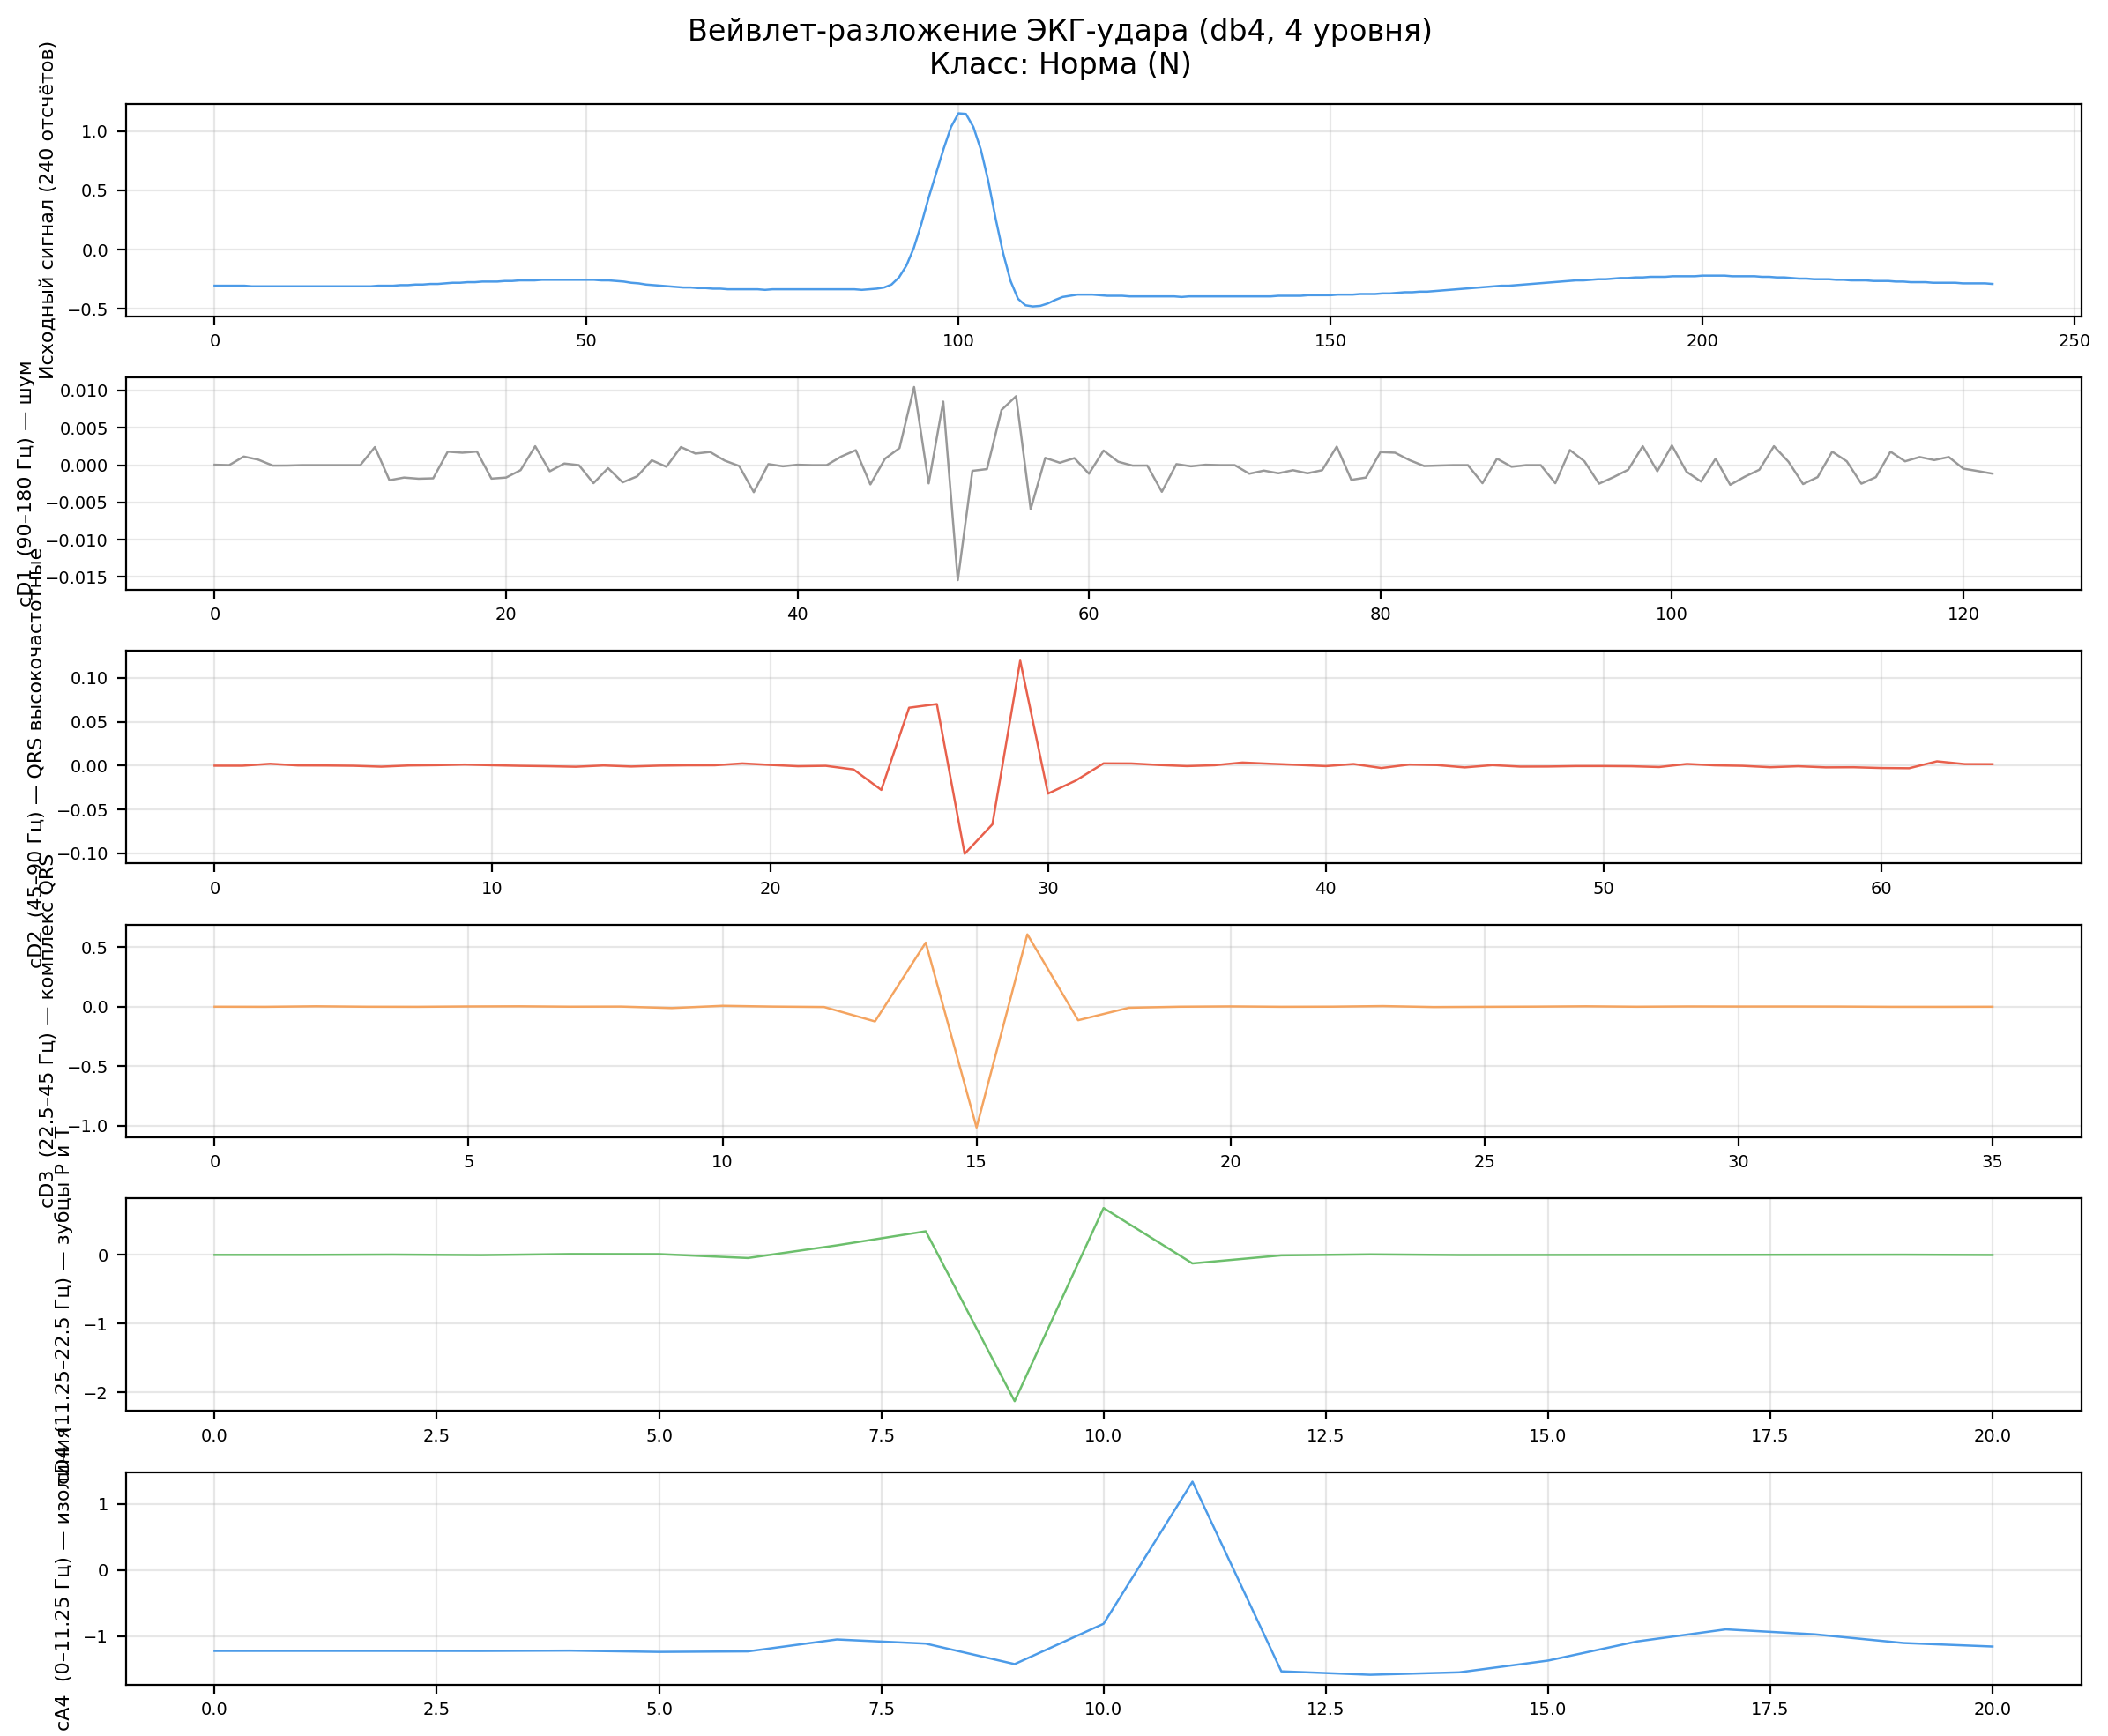
\includegraphics[width=0.85\textwidth]{../reports/figures/models/wavelet_decomposition_N.png}
\caption{Вейвлет-разложение нормального кардиоцикла (класс~N):
исходный сигнал и уровни ДВП db4.
По оси абсцисс~--- номер отсчета; по оси ординат~--- амплитуда в~мВ.}
\label{fig:beat_window}
\end{figure}

\subsubsection{Нормализация}

Для~нейронных сетей каждый признак нормализуется по~обучающей выборке
с~помощью стандартного масштабирования:
\begin{equation}
    \label{eq:scaler}
    \tilde{x}_{ij} = \frac{x_{ij} - \hat{\mu}_j}{\hat{\sigma}_j}\,,
    \quad j = 1, \ldots, d,
\end{equation}
где $\hat{\mu}_j$ и~$\hat{\sigma}_j$~--- выборочные среднее и~стандартное
отклонение $j$-го признака по~обучающей выборке.
Параметры нормализации вычисляются исключительно на~обучающих данных
и~применяются к~тестовой выборке без повторной подгонки~---
во~избежание «утечки» информации из~теста.
Для~случайного леса нормализация не~требуется, поскольку деревья
решений инвариантны к~монотонным преобразованиям признаков.

\subsection{Разбиение на выборки}

Выборка разбивается на~обучающую $(80\,\%)$ и~тестовую $(20\,\%)$
части методом стратифицированного разбиения:
\begin{equation}
    |\mathcal{D}_\text{train}| = 80\,020, \quad
    |\mathcal{D}_\text{test}| = 20\,005.
\end{equation}
Стратификация гарантирует, что~доля каждого класса в~обеих частях
совпадает с~долей в~исходной выборке.
Фиксированный начальный номер генератора случайных чисел
(\texttt{random\_state=42}) обеспечивает воспроизводимость результатов.

Для~оценки стабильности моделей дополнительно проводится
пятикратная стратифицированная кросс-валидация~(см.~раздел~\ref{sec:Chapter4}).

\subsection{Проблема дисбаланса классов и способы ее решения}

Сильный дисбаланс классов~--- в~первую очередь малочисленность
класса~A~--- порождает систематическое смещение модели в~пользу
большинства: модель, предсказывающая «норму» для~всех объектов,
достигает Accuracy~$\approx 75\,\%$, оставаясь при~этом клинически
бесполезной.

В~данной работе применяются два независимых механизма компенсации
дисбаланса:

\begin{enumerate}
    \item \textbf{Взвешенная функция потерь} для~нейронных сетей.
    Каждому классу~$k$ назначается вес, обратно пропорциональный
    его частоте в~обучающей выборке:
    \begin{equation}
        \label{eq:weights}
        w_k = \frac{1/n_k}{\sum_{j \in \mathcal{Y}} 1/n_j}
        \cdot |\mathcal{Y}|,
    \end{equation}
    где $n_k$~--- число объектов класса~$k$ в~обучающей части.
    Взвешенная кросс-энтропия:
    \begin{equation}
        \label{eq:wce}
        \mathcal{L} = -\sum_{k \in \mathcal{Y}} w_k \sum_{i:\,y_i=k}
        \log \hat{p}_{ik},
    \end{equation}
    где $\hat{p}_{ik}$~--- предсказанная вероятность класса~$k$
    для~объекта~$i$.

    \item \textbf{Стратегия \texttt{balanced\_subsample}} для~случайного
    леса: при~построении каждого дерева обучающая выборка
    для~бутстрэпа ресамплируется с~равномерным представлением
    всех классов.
\end{enumerate}

\subsection{Требования к решению}

По~итогам работы решение должно удовлетворять следующим требованиям:

\begin{itemize}
    \item Macro~F1 не~ниже $0.90$ на~тестовой выборке для каждой
          из~трех моделей.
    \item Recall класса~A (предсердная экстрасистола) не~ниже $0.65$~---
          клинически значимое нарушение не~должно систематически
          пропускаться.
    \item Стандартное отклонение Macro~F1 по~фолдам кросс-валидации
          не~выше~$0.03$~--- требование к~стабильности модели.
    \item Модели должны быть сохранены в~воспроизводимом формате
          для~последующего применения на~новых записях.
\end{itemize}
 % Постановка задачи и описание данных
\section{Методы классификации биосигналов}
\label{sec:Chapter2}

В~данном разделе описываются три модели машинного обучения,
реализованные в~работе, а~также метод вейвлет-анализа,
применявшийся для~частотно-временного исследования ЭКГ-сигналов.

\subsection{Случайный лес}

\subsubsection{Алгоритм}

Случайный лес~(Random Forest)~\cite{breiman2001}~--- ансамблевый
метод, основанный на~бэггинге над~деревьями решений.
Для~задачи классификации с~$T$ деревьями ответ модели определяется
голосованием большинства:
\begin{equation}
    \hat{y} = \operatorname*{arg\,max}_{k \in \mathcal{Y}}
    \sum_{t=1}^{T} \mathbf{1}[\,h_t(\mathbf{x}) = k\,],
\end{equation}
где $h_t(\mathbf{x})$~--- предсказание $t$-го дерева.

Каждое дерево обучается на~бутстрэп-выборке из~обучающих данных,
а~при~выборе оптимального разбиения в~каждом узле рассматривается
случайное подмножество $m \approx \sqrt{d}$ признаков.
Такая рандомизация снижает корреляцию между деревьями и~уменьшает
дисперсию ансамбля~\cite{breiman2001}.

\subsubsection{Настройка гиперпараметров}

В~работе используется $T = 200$ деревьев.
Для~компенсации дисбаланса классов применяется стратегия
\texttt{balanced\_subsample}: при~формировании каждого
бутстрэп-экземпляра производится стратифицированная
ресамплировка, обеспечивающая равное число объектов каждого
класса в~обучающей порции дерева.
Функционал информативности узла~--- критерий Джини.

\subsubsection{Важность признаков}

Случайный лес позволяет оценить вклад каждого признака $j$
в~качество классификации через среднее уменьшение примеси~(MDI):
\begin{equation}
    \mathrm{Imp}(j) = \frac{1}{T}\sum_{t=1}^{T}
    \sum_{\text{узлы с разб.\ по }j}
    \Delta\mathrm{Gini}_t \cdot \frac{n_\text{узел}}{n},
\end{equation}
где $\Delta\mathrm{Gini}_t$~--- уменьшение индекса Джини в~узле.
Анализ важности признаков позволяет интерпретировать, какие
временны\'{е} участки кардиоцикла наиболее информативны
при~разделении классов.

\subsection{Одномерная сверточная нейронная сеть (1D CNN)}

\subsubsection{Мотивация}

Сверточные нейронные сети~\cite{lecun1998} обладают свойством
\textit{трансляционной инвариантности}: один и~тот~же паттерн
формы QRS-комплекса обнаруживается вне~зависимости от~его
положения в~окне.
Применение одномерных сверток к~временному ряду ЭКГ позволяет
автоматически извлекать иерархические признаки: от~низкоуровневых
перепадов амплитуды до~высокоуровневых форм зубцов.

\subsubsection{Архитектура}

Входной тензор имеет форму $(\text{batch},\,1,\,240)$~---
один канал, $240$ временны\'{х} отсчетов.
Сеть состоит из~\textit{сверточного} блока и~\textit{классификатора}
(таблица~\ref{tab:cnn_arch}).

\begin{table}[h]
\centering
\caption{Архитектура 1D~CNN}
\label{tab:cnn_arch}
\begin{tabular}{llrr}
\hline
\textbf{Слой} & \textbf{Параметры} &
\textbf{Выход $(C \times L)$} & \textbf{Параметры, шт.} \\
\hline
Conv1d       & $1\to16$, $k=7$, $p=3$ & $16\times240$ & 128  \\
BatchNorm1d  & $16$                   & $16\times240$ & 32   \\
ReLU         & ---                    & $16\times240$ & 0    \\
MaxPool1d    & $k=2$                  & $16\times120$ & 0    \\
\hline
Conv1d       & $16\to32$, $k=5$, $p=2$ & $32\times120$ & 2\,592 \\
BatchNorm1d  & $32$                    & $32\times120$ & 64    \\
ReLU         & ---                     & $32\times120$ & 0     \\
MaxPool1d    & $k=2$                   & $32\times60$  & 0     \\
\hline
Conv1d       & $32\to64$, $k=5$, $p=2$ & $64\times60$ & 10\,304 \\
BatchNorm1d  & $64$                     & $64\times60$ & 128     \\
ReLU         & ---                      & $64\times60$ & 0       \\
MaxPool1d    & $k=2$                    & $64\times30$ & 0       \\
\hline
Flatten      & ---                      & $1920$       & 0       \\
Linear       & $1920\to128$             & $128$        & 245\,888 \\
ReLU         & ---                      & $128$        & 0        \\
Dropout      & $p=0.3$                  & $128$        & 0        \\
Linear       & $128\to5$                & $5$          & 645      \\
\hline
\multicolumn{3}{l}{\textbf{Итого обучаемых параметров}} & \textbf{259\,781} \\
\hline
\end{tabular}
\end{table}

Три стадии свертки с~попарным пулингом уменьшают длину
временного ряда с~$240$ до~$30$ отсчетов, одновременно
увеличивая число карт признаков с~$1$ до~$64$.
Регуляризация достигается через~BatchNorm после~каждой свертки
и~Dropout ($p=0.3$) перед выходным слоем.

\subsubsection{Обучение}

Оптимизатор~--- Adam~\cite{kingma2014} с~начальной скоростью обучения
$\eta_0 = 10^{-3}$.
Планировщик ReduceLROnPlateau снижает $\eta$ вдвое, если Macro~F1
на~валидации не~улучшается в~течение $3$~эпох:
$\eta \leftarrow 0.5\,\eta$.
Ранняя остановка с~patience~$=5$ предотвращает переобучение.
Число эпох~--- не~более~$20$; наилучшие веса по~Macro~F1 сохраняются
отдельно.

\subsection{Остаточная нейронная сеть (ResNet1D)}

\subsubsection{Мотивация и остаточное соединение}

При~увеличении глубины нейронной сети возникает проблема
затухающих градиентов: сигнал ошибки, распространяясь в~обратном
направлении, многократно умножается на~небольшие числа и~«исчезает»
в~ранних слоях~\cite{goodfellow2016}.
He~и~др.~\cite{he2016} предложили архитектуру с~\textit{остаточными
соединениями} (skip connections), вычисляющую не~прямое
отображение $H(\mathbf{x})$, а~остаток $F(\mathbf{x})$:
\begin{equation}
    \label{eq:residual}
    \mathbf{y} = F(\mathbf{x},\,\{W_i\}) + \mathbf{x},
\end{equation}
где $F(\mathbf{x})$~--- нелинейное преобразование двух сверточных
слоев, а~$\mathbf{x}$~--- прямая «шунтирующая» ветвь.
Такое соединение устраняет проблему затухания и~позволяет
обучать существенно более глубокие сети.

\subsubsection{Архитектура}

Реализованная модель ResNet1D состоит из~начального стволового
слоя (\textit{stem}) и~трех остаточных блоков
(таблица~\ref{tab:resnet_arch}).

\begin{table}[h]
\centering
\caption{Архитектура ResNet1D}
\label{tab:resnet_arch}
\begin{tabular}{lllr}
\hline
\textbf{Блок} & \textbf{Состав} & \textbf{Выход $(C \times L)$} &
\textbf{stride} \\
\hline
Stem     & Conv1d($1\to16$, $k=7$) + BN + ReLU & $16\times240$ & 1 \\
\hline
Layer\,1 & ResidualBlock($16\to16$, $k=7$)     & $16\times240$ & 1 \\
Layer\,2 & ResidualBlock($16\to32$, $k=7$)     & $32\times120$ & 2 \\
Layer\,3 & ResidualBlock($32\to64$, $k=7$)     & $64\times60$  & 2 \\
\hline
Pool     & AdaptiveAvgPool1d(1)                 & $64\times1$   & --- \\
FC       & Linear($64\to5$)                    & $5$           & --- \\
\hline
\end{tabular}
\end{table}

Каждый \textit{ResidualBlock} содержит две последовательные
свертки с~BatchNorm и~ReLU, а~также адаптивный шунт:
если размерности входа и~выхода не~совпадают (по~каналам или
длине), шунт реализуется сверткой $1\times1$ со~stride; иначе~---
тождественным отображением (Identity).
После сложения $F(\mathbf{x}) + \text{shortcut}(\mathbf{x})$
применяется ReLU.

Слой \texttt{AdaptiveAvgPool1d(1)} глобально усредняет
карту признаков по~временному измерению, что~делает сеть
нечувствительной к~его абсолютной длине.
Итоговый вектор из~$64$ нейронов подается в~линейный
классификатор.

\subsubsection{Обучение}

Конфигурация обучения аналогична CNN: оптимизатор Adam
($\eta_0 = 10^{-3}$), взвешенная кросс-энтропия
(формулы~\eqref{eq:weights},~\eqref{eq:wce}),
ReduceLROnPlateau~($\times0.5$, patience~$=3$),
ранняя остановка (patience~$=7$), не~более~$30$~эпох.
Перед обучением признаки нормализуются по~формуле~\eqref{eq:scaler},
параметры нормализации сохраняются для~последующей оценки.

\subsection{Вейвлет-анализ ЭКГ-сигналов}

\subsubsection{Ограничения преобразования Фурье}

Классическое преобразование Фурье дает полную информацию
о~частотном составе сигнала, но~не~позволяет установить,
\textit{в~какой момент времени} та~или~иная частота присутствует.
Поскольку ЭКГ является нестационарным сигналом~--- его
характеристики меняются на~протяжении одного кардиоцикла
(зубцы~P, QRS, T имеют различные частотные составы)~---
для~его анализа требуется инструмент совместного
частотно-временного представления~\cite{zakharova2018}.

\subsubsection{Дискретное вейвлет-преобразование}

Дискретное вейвлет-преобразование~(ДВП) разлагает сигнал
$s[n]$ по~ортонормированному базису масштабирующих функций
и~вейвлетов методом пирамидального алгоритма Малла~\cite{mallat1989}.
На~каждом уровне разложения $j$ сигнал пропускается
через пару фильтров: фильтр нижних частот дает
коэффициенты приближения~$\{a_j[n]\}$, фильтр верхних частот~---
коэффициенты детализации~$\{d_j[n]\}$:
\begin{equation}
    a_j[n] = \sum_k h[k]\, a_{j-1}[2n-k], \quad
    d_j[n] = \sum_k g[k]\, a_{j-1}[2n-k],
\end{equation}
где $h[k]$ и~$g[k]$~--- коэффициенты квадратурных зеркальных
фильтров, определяемых выбором вейвлета.

В~работе используется вейвлет Добеши~4 (db4), обладающий
$4$~нулевыми моментами~--- что~обеспечивает компактную
запись гладких сигналов~--- и~хорошо согласованный
с~формой QRS-комплекса~\cite{zakharova2018}.
При~$L = 4$ уровнях разложения и~частоте дискретизации
$f_s = 360$~Гц формируются следующие частотные подполосы
(таблица~\ref{tab:wavelet_bands}).

\begin{table}[h]
\centering
\caption{Частотные подполосы ДВП db4 при $f_s = 360$~Гц}
\label{tab:wavelet_bands}
\begin{tabular}{clll}
\hline
\textbf{Подполоса} & \textbf{Частоты, Гц} & \textbf{Физ.\ смысл для ЭКГ} &
\textbf{Число коэф.} \\
\hline
$\mathrm{cD}_1$ & $90\text{–}180$ & Высокочастотный шум (ЭМГ) & $\approx 120$ \\
$\mathrm{cD}_2$ & $45\text{–}90$  & Высокочаст.\ компоненты QRS  & $\approx 60$ \\
$\mathrm{cD}_3$ & $22.5\text{–}45$& Комплекс QRS                 & $\approx 30$ \\
$\mathrm{cD}_4$ & $11\text{–}22.5$& Зубцы P и T                  & $\approx 15$ \\
$\mathrm{cA}_4$ & $0\text{–}11$   & Изолиния, дрейф              & $\approx 15$ \\
\hline
\end{tabular}
\end{table}

\subsubsection{Вейвлет-признаки для случайного леса}

Для~расширения векторного представления каждого кардиоцикла
из~коэффициентов каждой подполосы~$\mathrm{cX}_j$ извлекаются
$5$ статистических признаков:
\begin{equation}
    \boldsymbol{\phi}(\mathrm{cX}_j) = \Bigl(
    \bar{c}_j,\;\sigma_j,\;E_j,\;\max|\mathrm{cX}_j|,\;\gamma_{1,j}
    \Bigr),
\end{equation}
где $\bar{c}_j$~--- среднее, $\sigma_j$~--- стандартное отклонение,
$E_j = \mathrm{mean}(\mathrm{cX}_j^2)$~--- энергия,
$\gamma_{1,j}$~--- коэффициент асимметрии.
Таким образом, каждый удар дополнительно описывается вектором
из~$5 \times 5 = 25$ вейвлет-признаков.

В~проведенном эксперименте (раздел~\ref{sec:Chapter3}) добавление
вейвлет-признаков к~$240$~временны\'{м} отсчетам не~улучшило
качество случайного леса: Macro~F1~$= 0.9479$ (с~вейвлетом)
против~$0.9496$ (без~него).
Это объясняется тем, что~ансамбль деревьев неявно обнаруживает
частотно-временны\'{е} паттерны непосредственно из~временного ряда,
тогда как~агрегатные статистики коэффициентов теряют позиционную
информацию.
Тем~не~менее вейвлет-анализ представляет значительную ценность
для~\textit{интерпретации} сигналов: скаллограммы~(рисунок~\ref{fig:cwt})
и~распределение энергии по~подполосам~(рисунок~\ref{fig:wt_energy})
наглядно демонстрируют, как~различные классы аритмий отличаются
в~частотно-временном пространстве.

\begin{figure}[h]
\centering
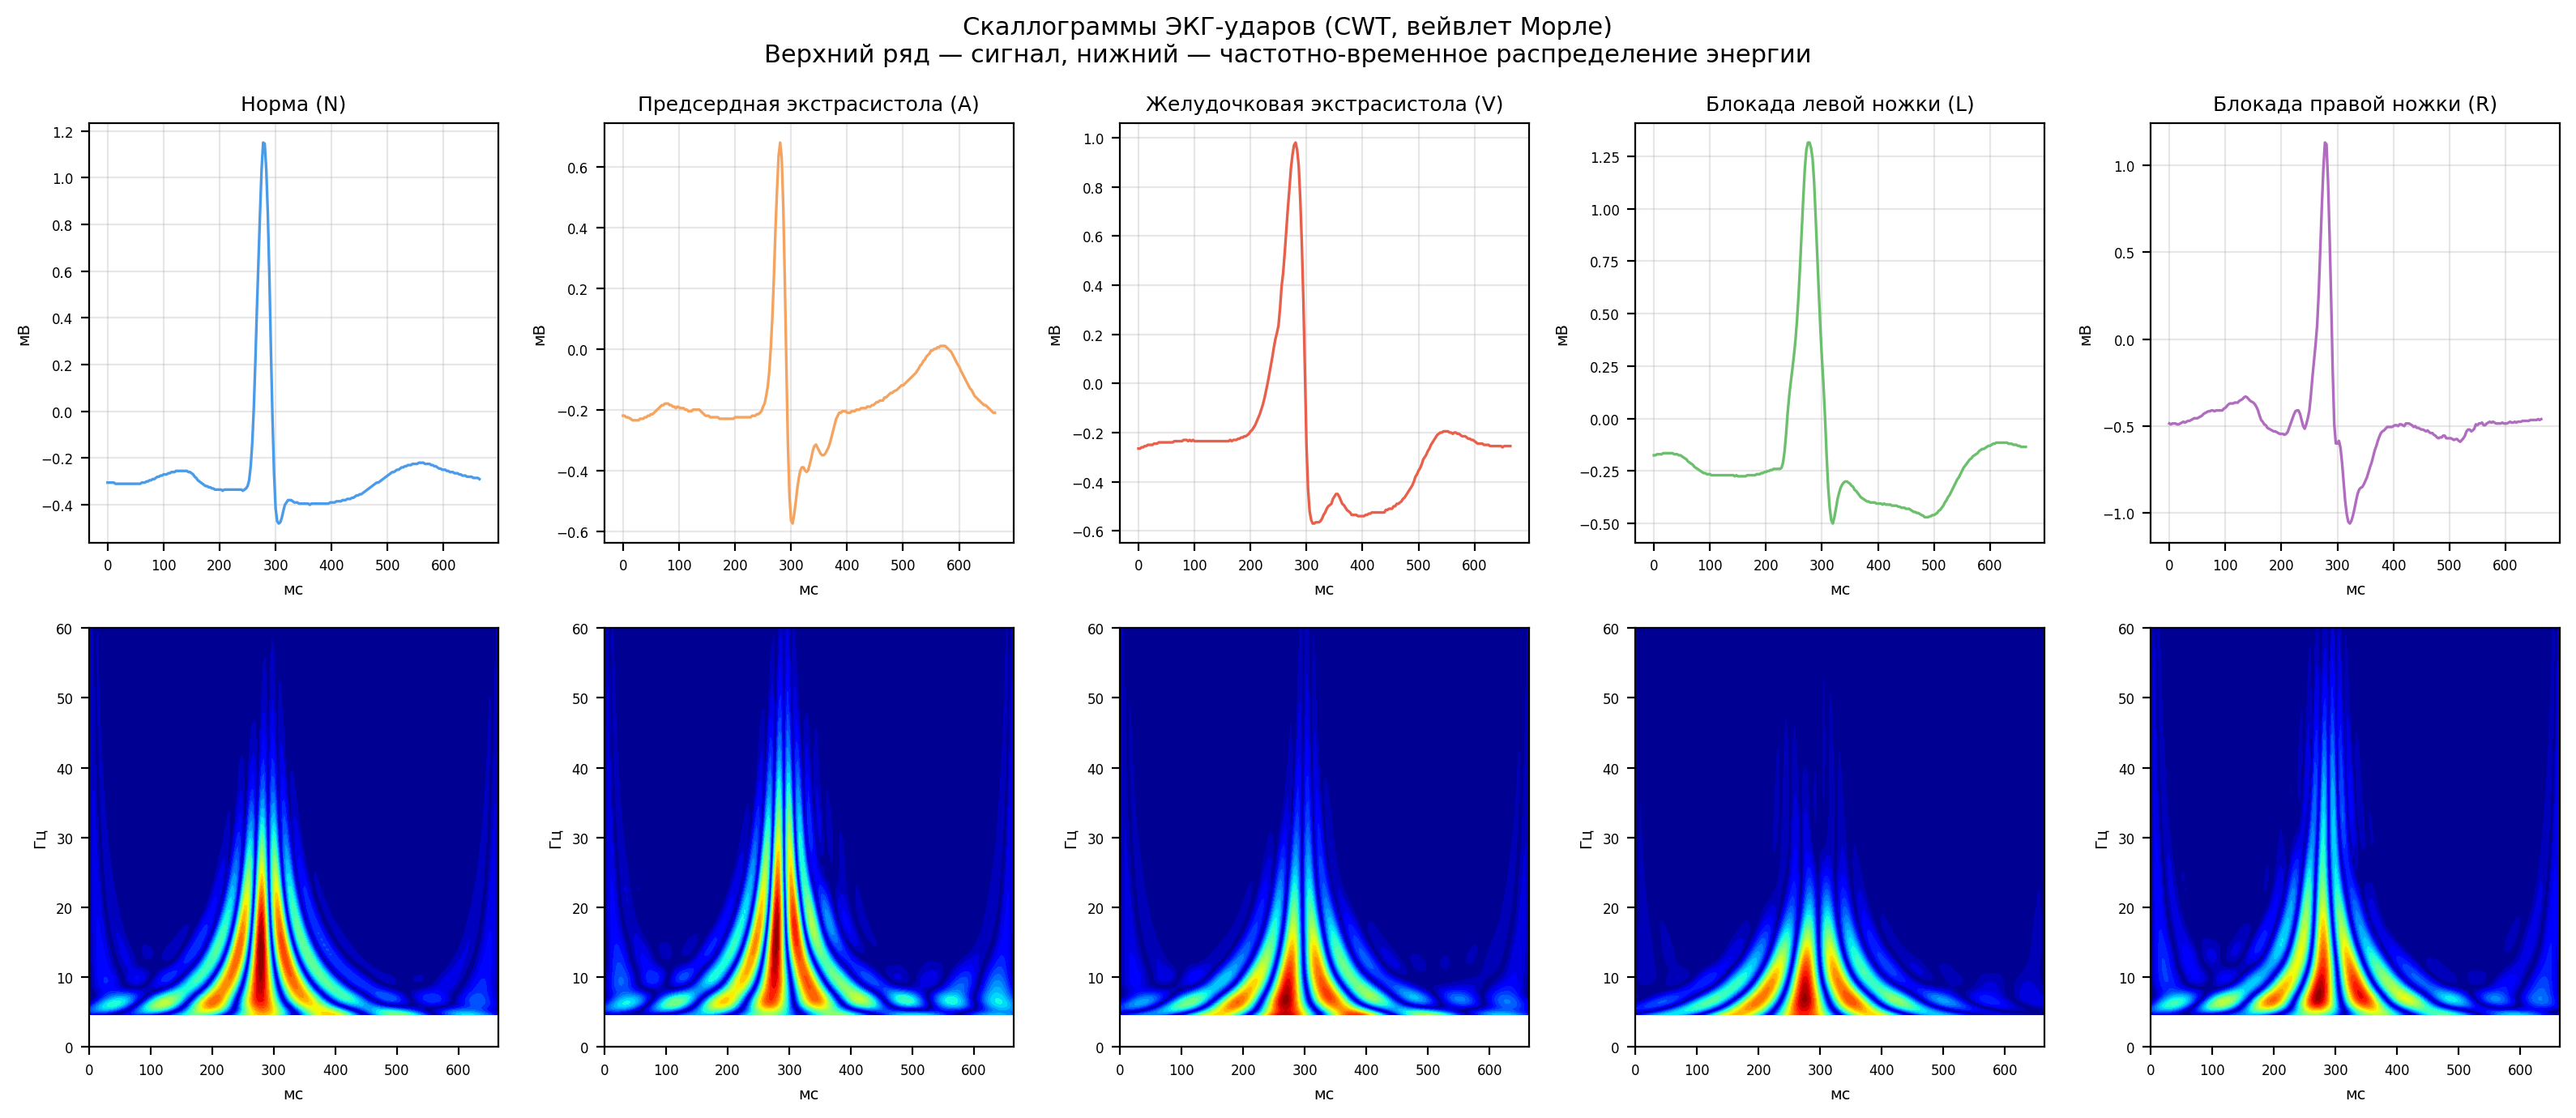
\includegraphics[width=\textwidth]{../reports/figures/models/wavelet_cwt_gallery.png}
\caption{Скаллограммы CWT (вейвлет Морле) для медианного удара каждого класса.
Верхний ряд~--- временной сигнал, нижний~--- частотно-временное распределение
энергии.}
\label{fig:cwt}
\end{figure}

\begin{figure}[h]
\centering
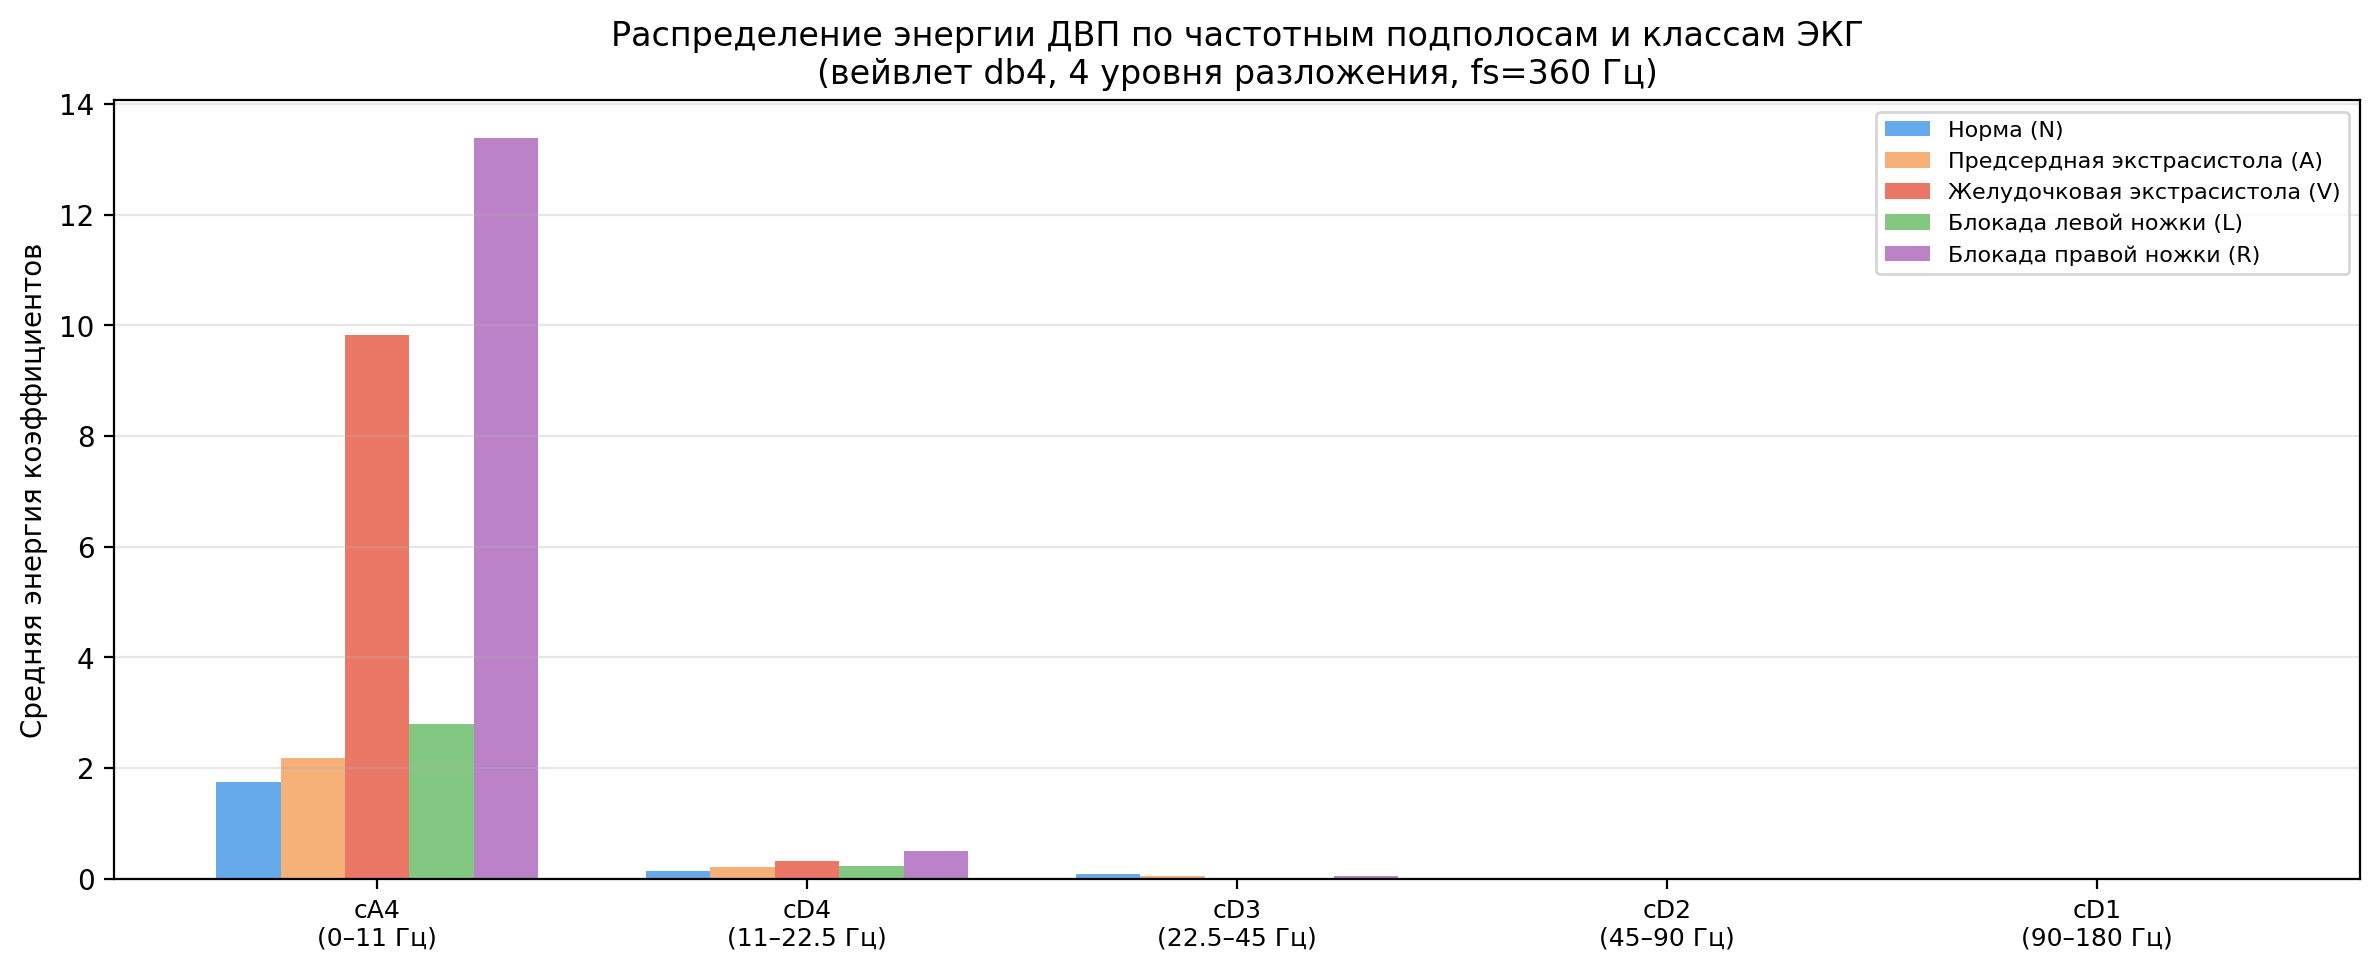
\includegraphics[width=0.95\textwidth]{../reports/figures/models/wavelet_avg_energy.png}
\caption{Средняя энергия коэффициентов ДВП db4 по~частотным подполосам и~классам.
Различие классов~V и~A в~подполосах $\mathrm{cD}_3$--$\mathrm{cD}_4$
отражает разницу в~форме QRS-комплекса.}
\label{fig:wt_energy}
\end{figure}

\subsection{Сравнительный анализ методов}

Три рассматриваемые модели занимают различные позиции
в~пространстве <<точность~--- интерпретируемость~--- устойчивость>>
(таблица~\ref{tab:model_comparison}).

\begin{table}[h]
\centering
\caption{Качественное сравнение моделей}
\label{tab:model_comparison}
\begin{tabular}{lccccc}
\hline
\textbf{Критерий} & \textbf{RF} & \textbf{1D~CNN} & \textbf{ResNet1D} \\
\hline
Интерпретируемость     & Высокая  & Низкая   & Низкая  \\
Нормализация           & Не нужна & Нужна    & Нужна   \\
Устойчивость к~шуму    & Высокая  & Средняя  & Средняя \\
Гиперпараметров        & Мало     & Умеренно & Много   \\
Время обучения         & Быстро   & Умеренно & Медленно \\
Качество (Macro~F1)    & 0.950    & \textbf{0.974}    & 0.953   \\
\hline
\end{tabular}
\end{table}

Случайный лес выигрывает по~простоте настройки и~интерпретируемости.
1D~CNN достигает наилучшего качества классификации за~счет
автоматического извлечения признаков.
ResNet1D потенциально мощнее, но~требует большего числа эпох
для~сходимости и~чувствителен к~инициализации.
 % Методы классификации биосигналов
\section{Результаты классификации на чистых данных}
\label{sec:Chapter3}

В~данном разделе приводятся результаты обучения и~тестирования
трех моделей на~исходных, незашумленных данных.
Все~эксперименты воспроизводимы: фиксированы начальный номер
генератора случайных чисел (\texttt{random\_state=42}),
разбиение на~выборки и~гиперпараметры.

\subsection{Сводная таблица метрик}

Результаты на~тестовой выборке ($|\mathcal{D}_\text{test}| = 20\,005$)
представлены в~таблице~\ref{tab:clean_results}.

\begin{table}[h]
\centering
\caption{Метрики качества моделей на~чистых данных}
\label{tab:clean_results}
\begin{tabular}{lccc}
\hline
\textbf{Модель} & \textbf{Accuracy} & \textbf{Macro F1} & \textbf{Weighted F1} \\
\hline
1D~CNN      & \textbf{0.9917} & \textbf{0.9736} & \textbf{0.9918} \\
ResNet1D    & 0.9847          & 0.9532          & 0.9848          \\
RandomForest & 0.9848         & 0.9496          & 0.9841          \\
\hline
\end{tabular}
\end{table}

Все~три модели превышают порог Macro~F1~$\geq 0.90$,
поставленный в~разделе~\ref{sec:Chapter1}.
Наилучший результат демонстрирует 1D~CNN (Macro~F1~$= 0.974$),
опережая ResNet1D на~$0.020$ и~Random Forest на~$0.024$.
Несмотря на~то что~Accuracy у~RF и~ResNet1D практически одинакова
($0.9848$ против~$0.9847$), Macro~F1 у~ResNet1D выше
($0.9532$ против~$0.9496$) за~счет лучшей работы
с~миноритарными классами.

\subsection{Анализ по классам: матрицы ошибок}

\subsubsection{1D CNN}

\begin{figure}[h]
\centering
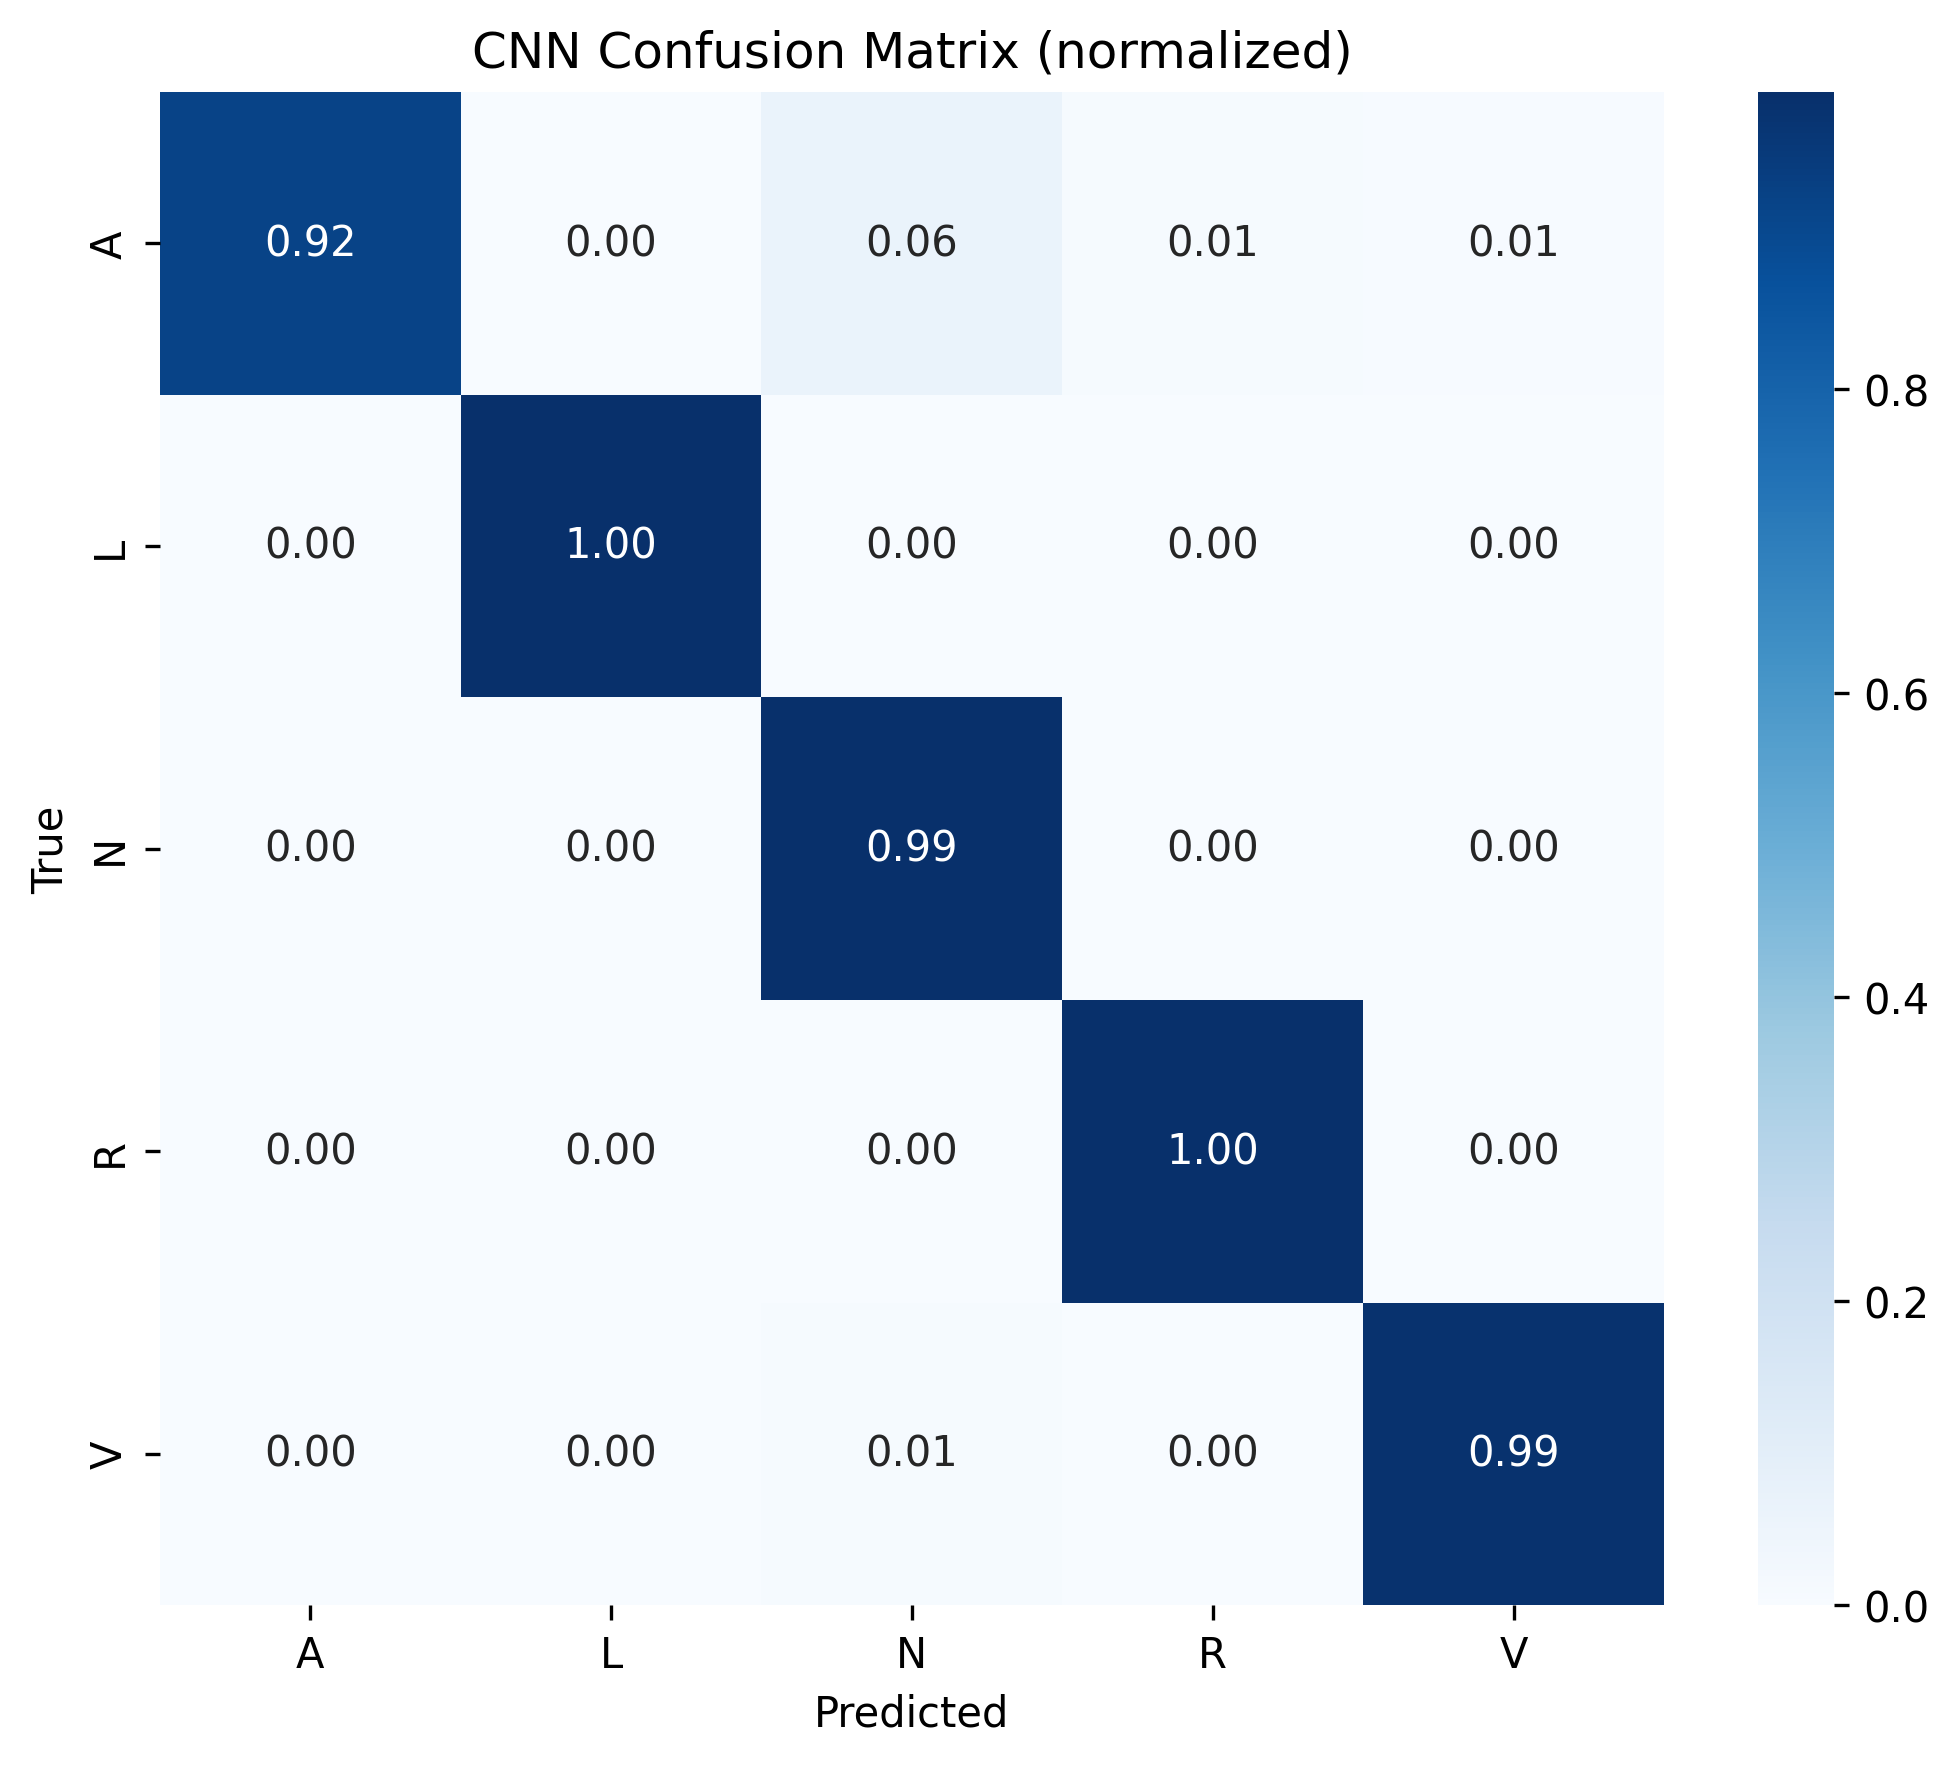
\includegraphics[width=0.65\textwidth]{../reports/figures/models/cm_cnn_normalized.png}
\caption{Нормализованная матрица ошибок 1D~CNN.
По диагонали~--- доля правильно классифицированных объектов каждого класса.}
\label{fig:cm_cnn}
\end{figure}

CNN добивается recall~$= 0.92$ для~класса~A~---
наилучший результат среди всех трех моделей.
Это достигается благодаря взвешенной функции потерь
(формула~\eqref{eq:wce}), которая увеличивает штраф
за~пропуск редких классов.
Классы~N, L, R распознаются практически безошибочно
(recall~$\geq 0.98$), класс~V~--- с~recall~$\approx 0.97$.

\subsubsection{ResNet1D}

\begin{figure}[h]
\centering
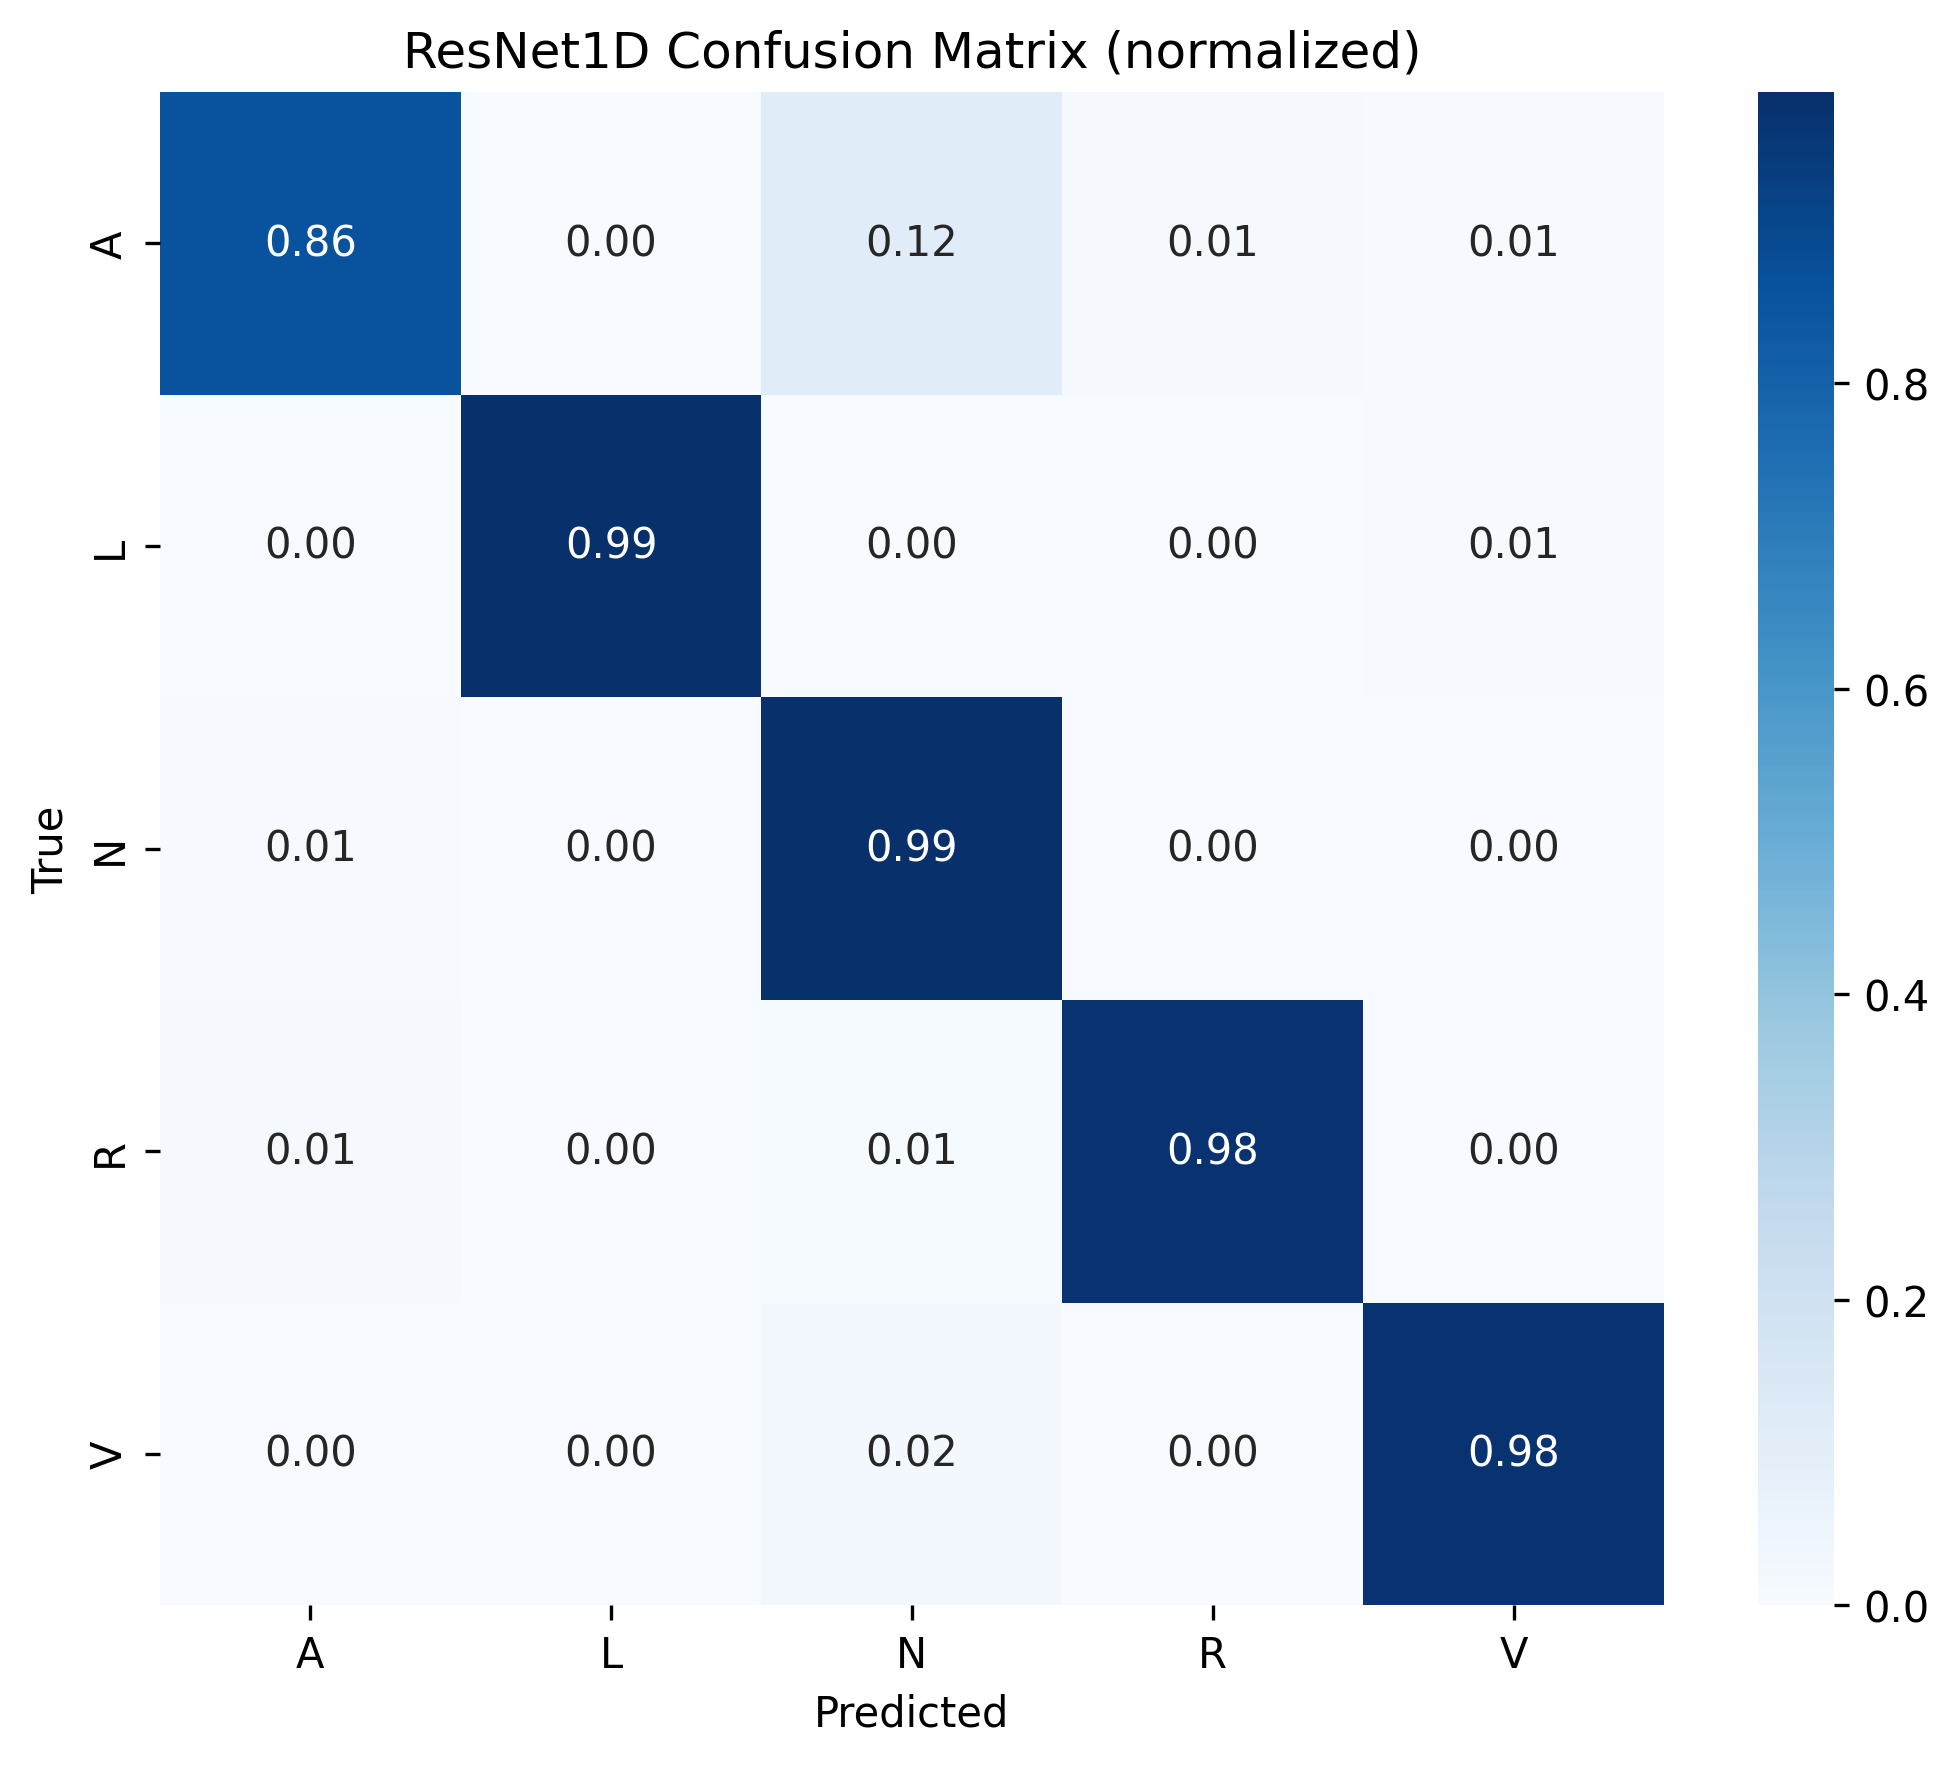
\includegraphics[width=0.65\textwidth]{../reports/figures/models/cm_resnet_normalized.png}
\caption{Нормализованная матрица ошибок ResNet1D.}
\label{fig:cm_resnet}
\end{figure}

ResNet1D устойчиво классифицирует классы~N, L, R, V
(recall~$\geq 0.94$).
Класс~A вызывает наибольшие затруднения: recall несколько ниже,
чем~у~CNN, что~объясняется меньшим числом эпох обучения
и~более сложной архитектурой, требующей большего времени сходимости.

\subsubsection{Random Forest}

\begin{figure}[h]
\centering
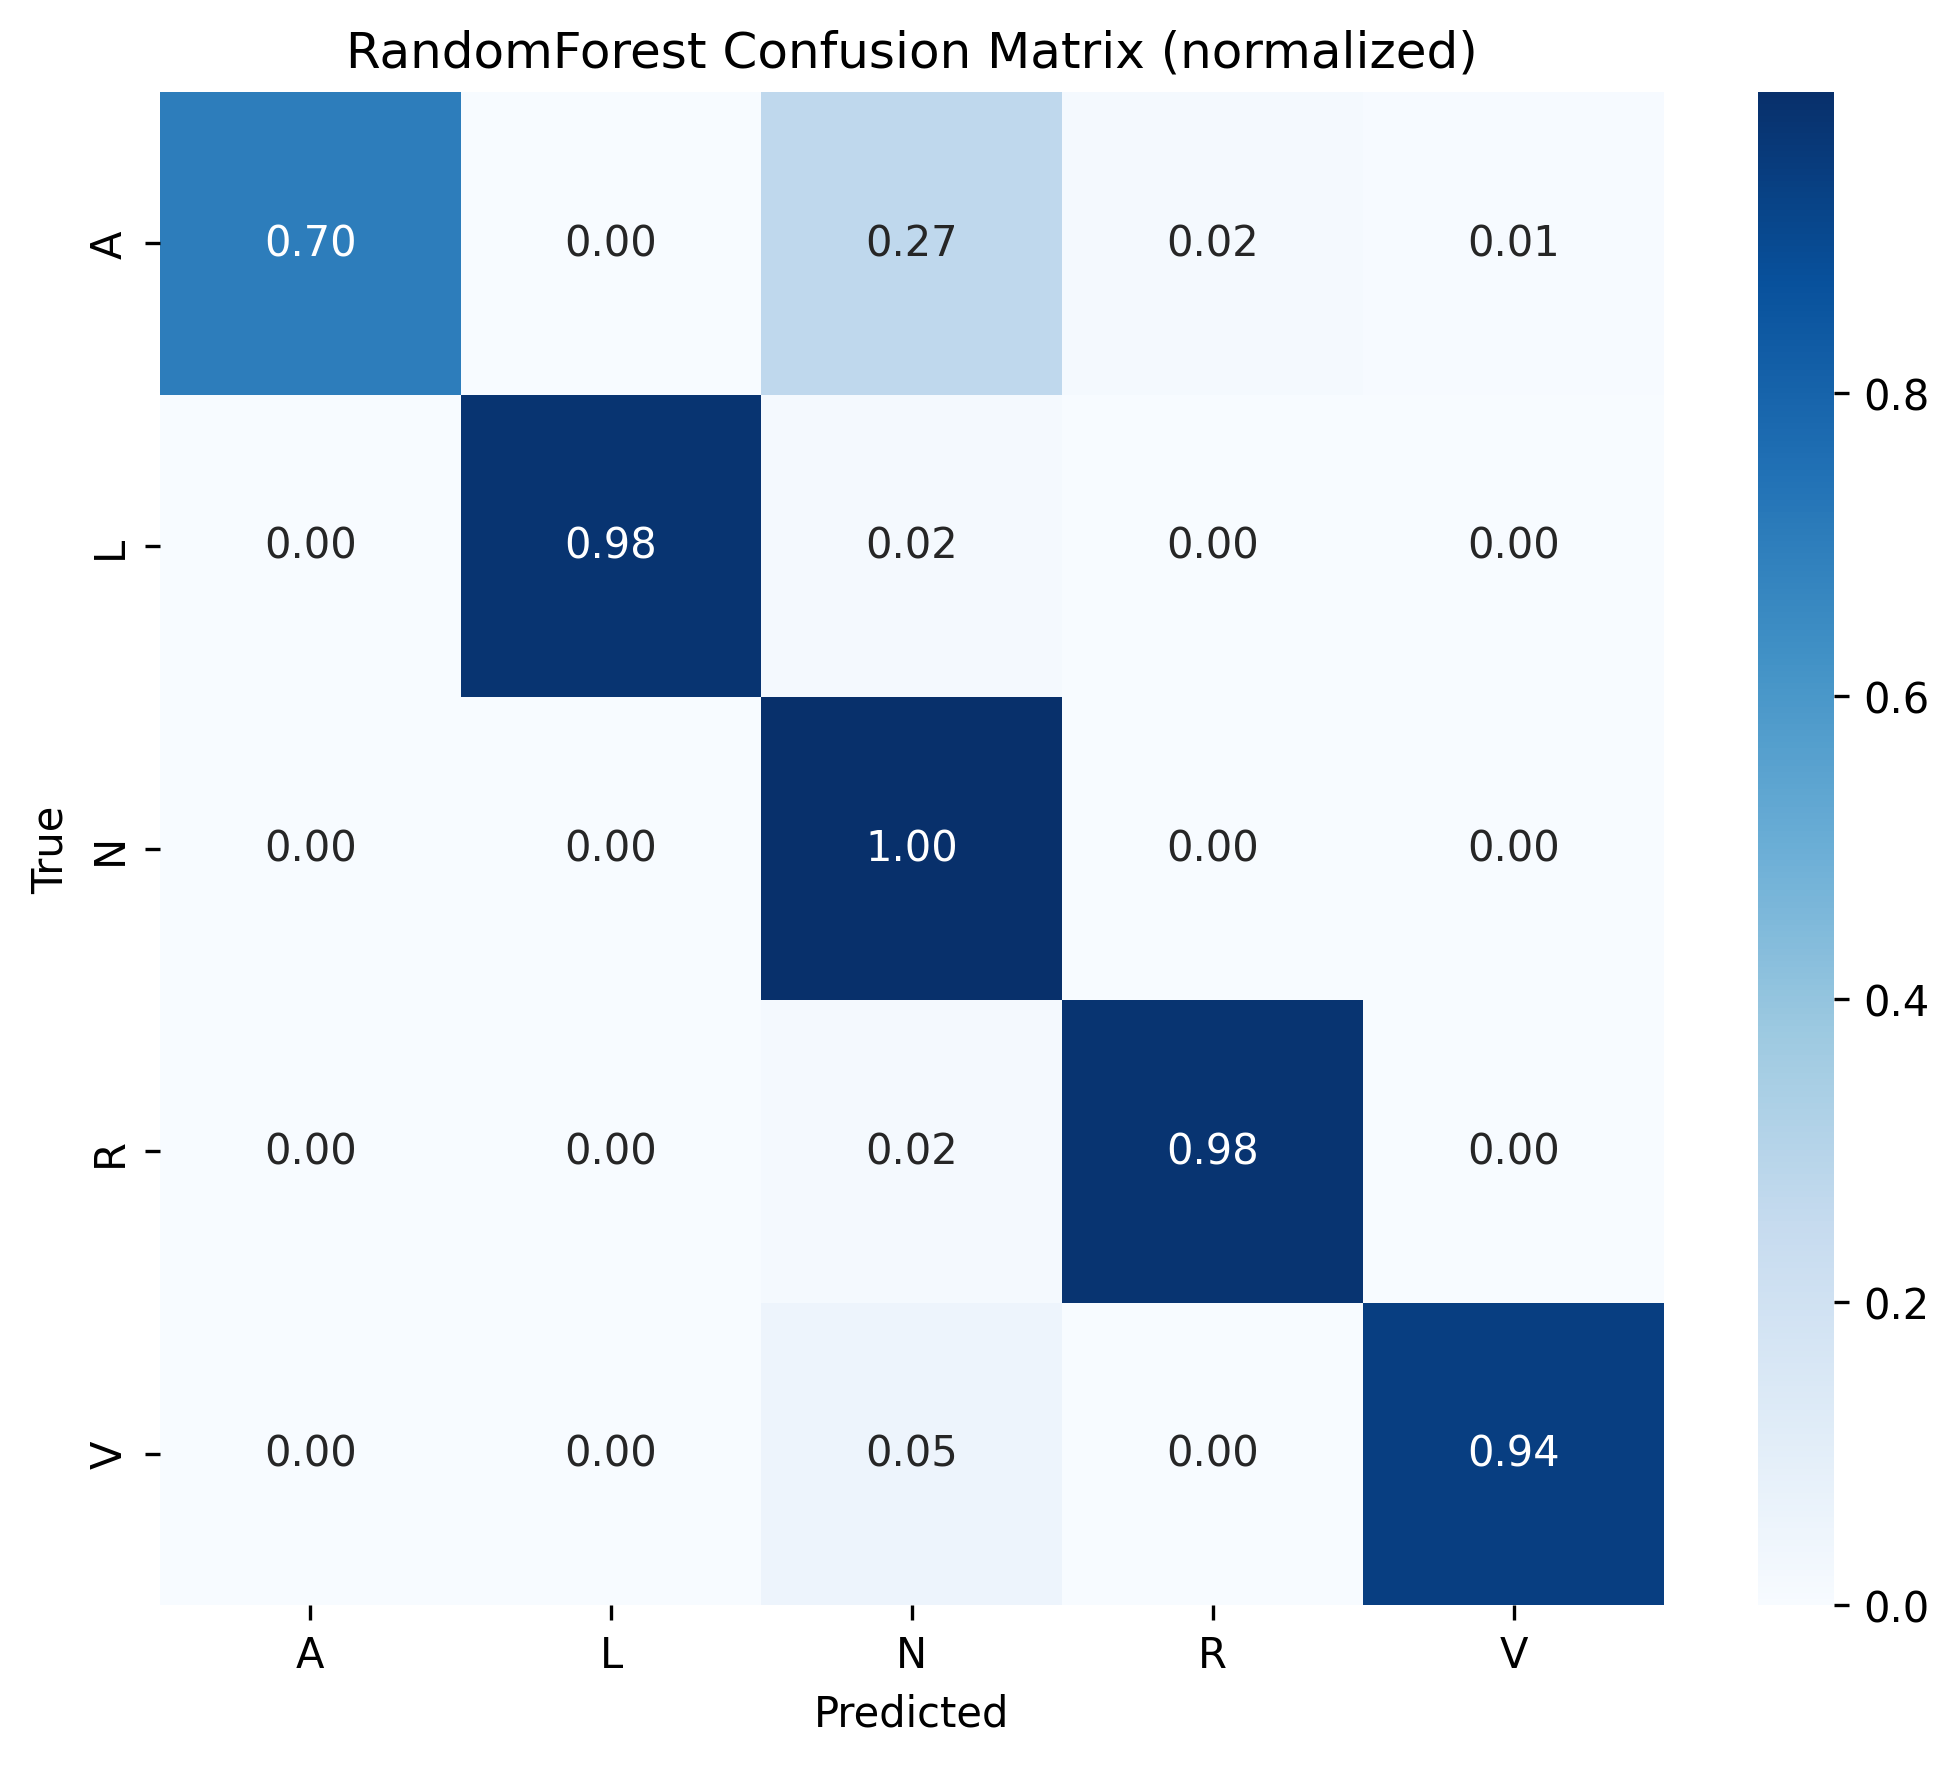
\includegraphics[width=0.65\textwidth]{../reports/figures/models/cm_rf_normalized.png}
\caption{Нормализованная матрица ошибок Random Forest.}
\label{fig:cm_rf}
\end{figure}

Главная слабость RF~--- recall класса~A~$= 0.70$:
каждый третий случай предсердной экстрасистолы пропускается.
Это существенный недостаток с~клинической точки зрения.
Стратегия \texttt{balanced\_subsample} частично компенсирует
дисбаланс, однако не~дает того эффекта, что~явное
взвешивание функции потерь у~нейронных сетей.
Классы~L, R, N распознаются надежно (recall~$\geq 0.98$).

\subsubsection{Сравнение по классу A}

Таблица~\ref{tab:class_a} обобщает результаты для~наиболее
проблематичного класса~A~--- предсердной экстрасистолы.

\begin{table}[h]
\centering
\caption{Метрики для класса A (предсердная экстрасистола)}
\label{tab:class_a}
\begin{tabular}{lcccc}
\hline
\textbf{Модель} & \textbf{Precision} & \textbf{Recall} &
\textbf{F1} & \textbf{Поддержка} \\
\hline
1D~CNN       & 0.96 & \textbf{0.92} & \textbf{0.94} & 509 \\
ResNet1D     & 0.95 & 0.88          & 0.91          & 509 \\
RandomForest & 0.98 & 0.70          & 0.82          & 509 \\
\hline
\end{tabular}
\end{table}

Все~модели удовлетворяют требованию recall(A)~$\geq 0.65$
из~постановки задачи (раздел~\ref{sec:Chapter1}).
CNN превышает этот порог с~запасом в~$0.27$.

\subsection{Кривые обучения нейронных сетей}

\subsubsection{1D CNN}

\begin{figure}[h]
\centering
\begin{minipage}{0.48\textwidth}
    \centering
    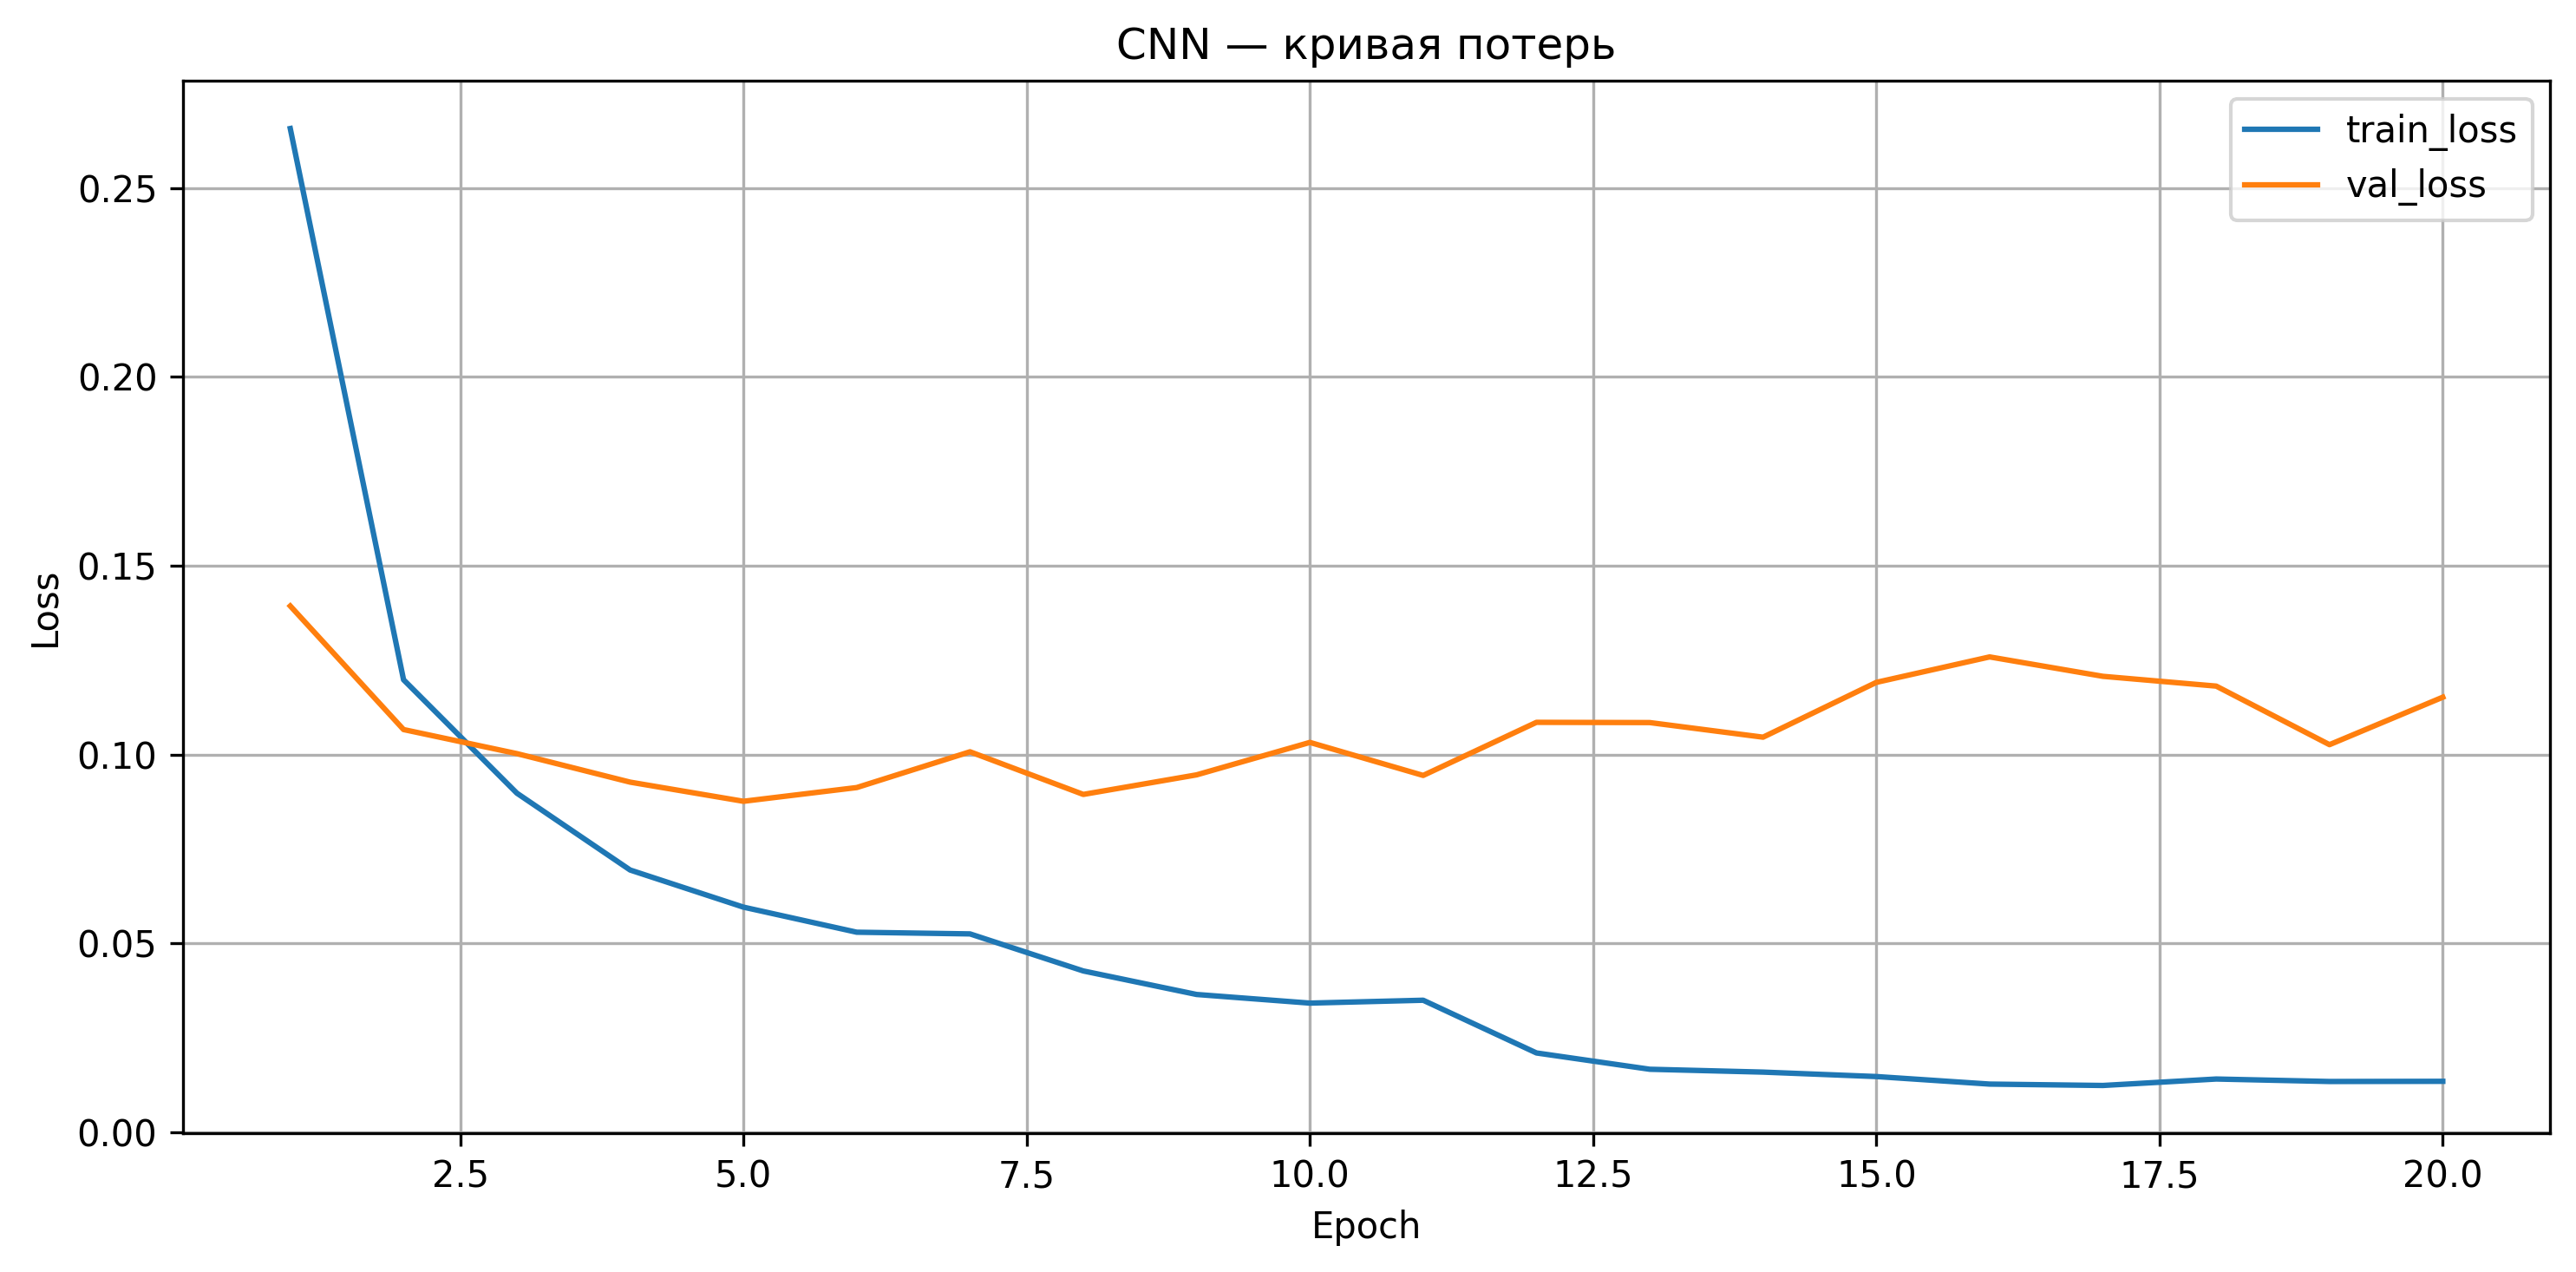
\includegraphics[width=\textwidth]{../reports/figures/models/cnn_loss_curve.png}
\end{minipage}
\hfill
\begin{minipage}{0.48\textwidth}
    \centering
    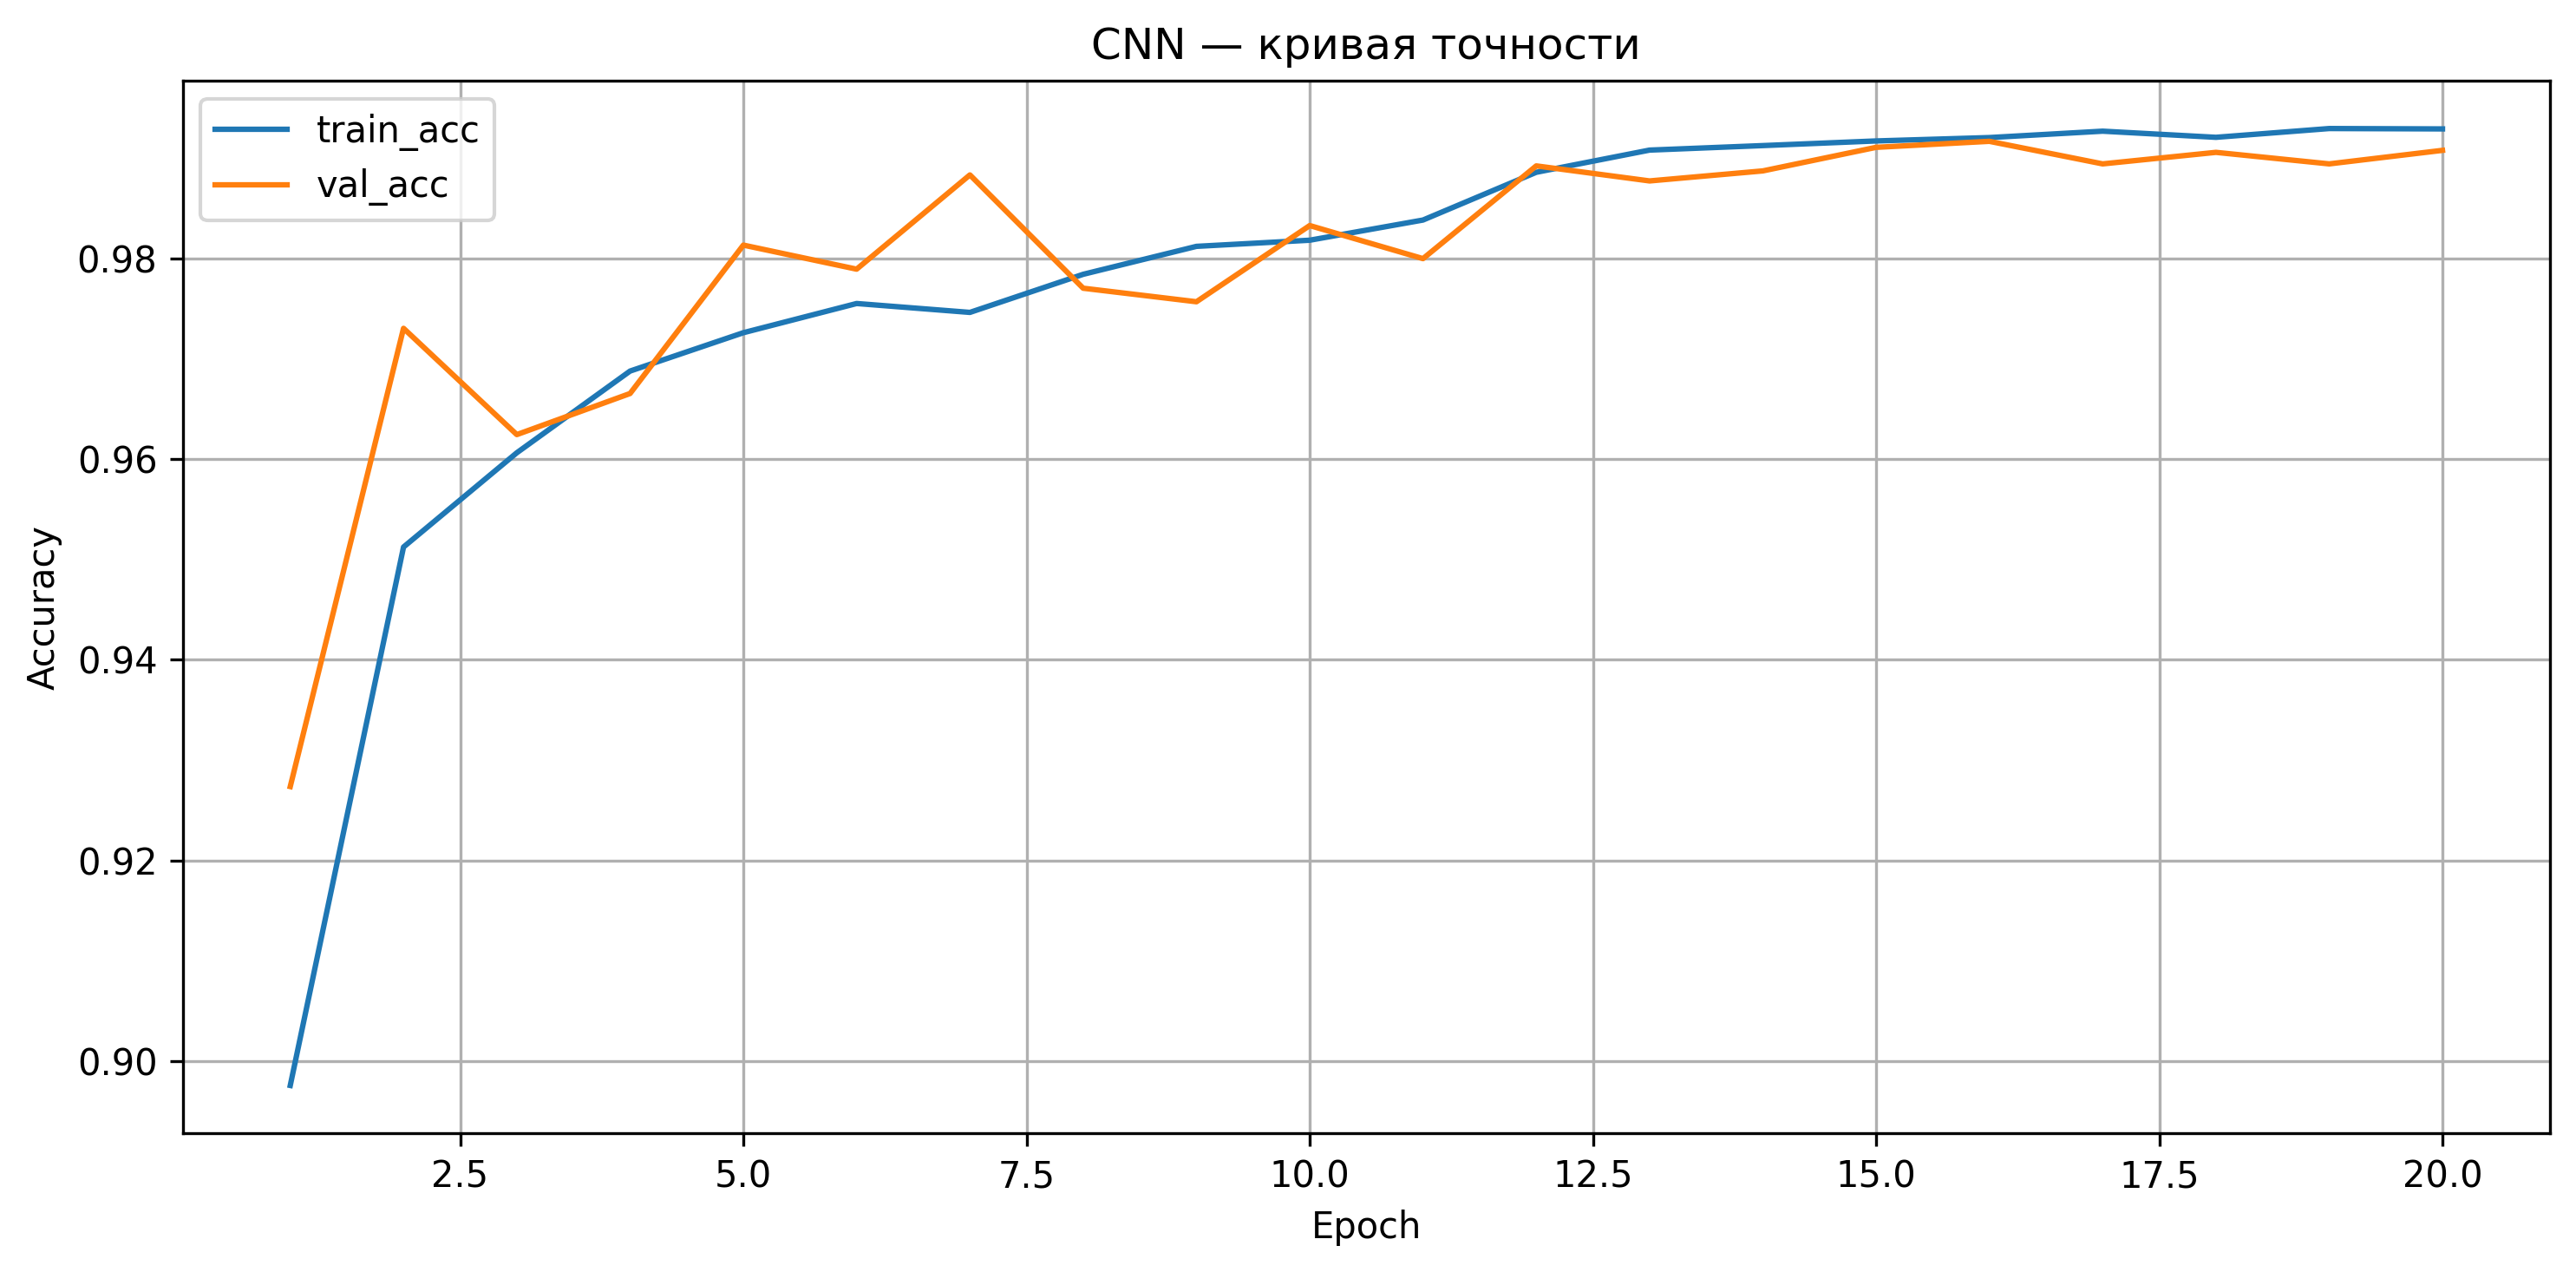
\includegraphics[width=\textwidth]{../reports/figures/models/cnn_accuracy_curve.png}
\end{minipage}
\caption{Кривые потерь (слева) и~точности (справа) 1D~CNN
в~процессе обучения. Вертикальная линия соответствует эпохе
ранней остановки.}
\label{fig:cnn_curves}
\end{figure}

Сеть сходится равномерно: валидационная и~обучающая кривые
идут вместе~--- признак отсутствия переобучения.
Механизм ReduceLROnPlateau снижает скорость обучения примерно
на~$10$--$12$~эпохе, что~проявляется в~характерном «перегибе»
кривой потерь.
Ранняя остановка фиксирует лучшие веса до~начала возможного
переобучения.

\subsubsection{ResNet1D}

\begin{figure}[h]
\centering
\begin{minipage}{0.48\textwidth}
    \centering
    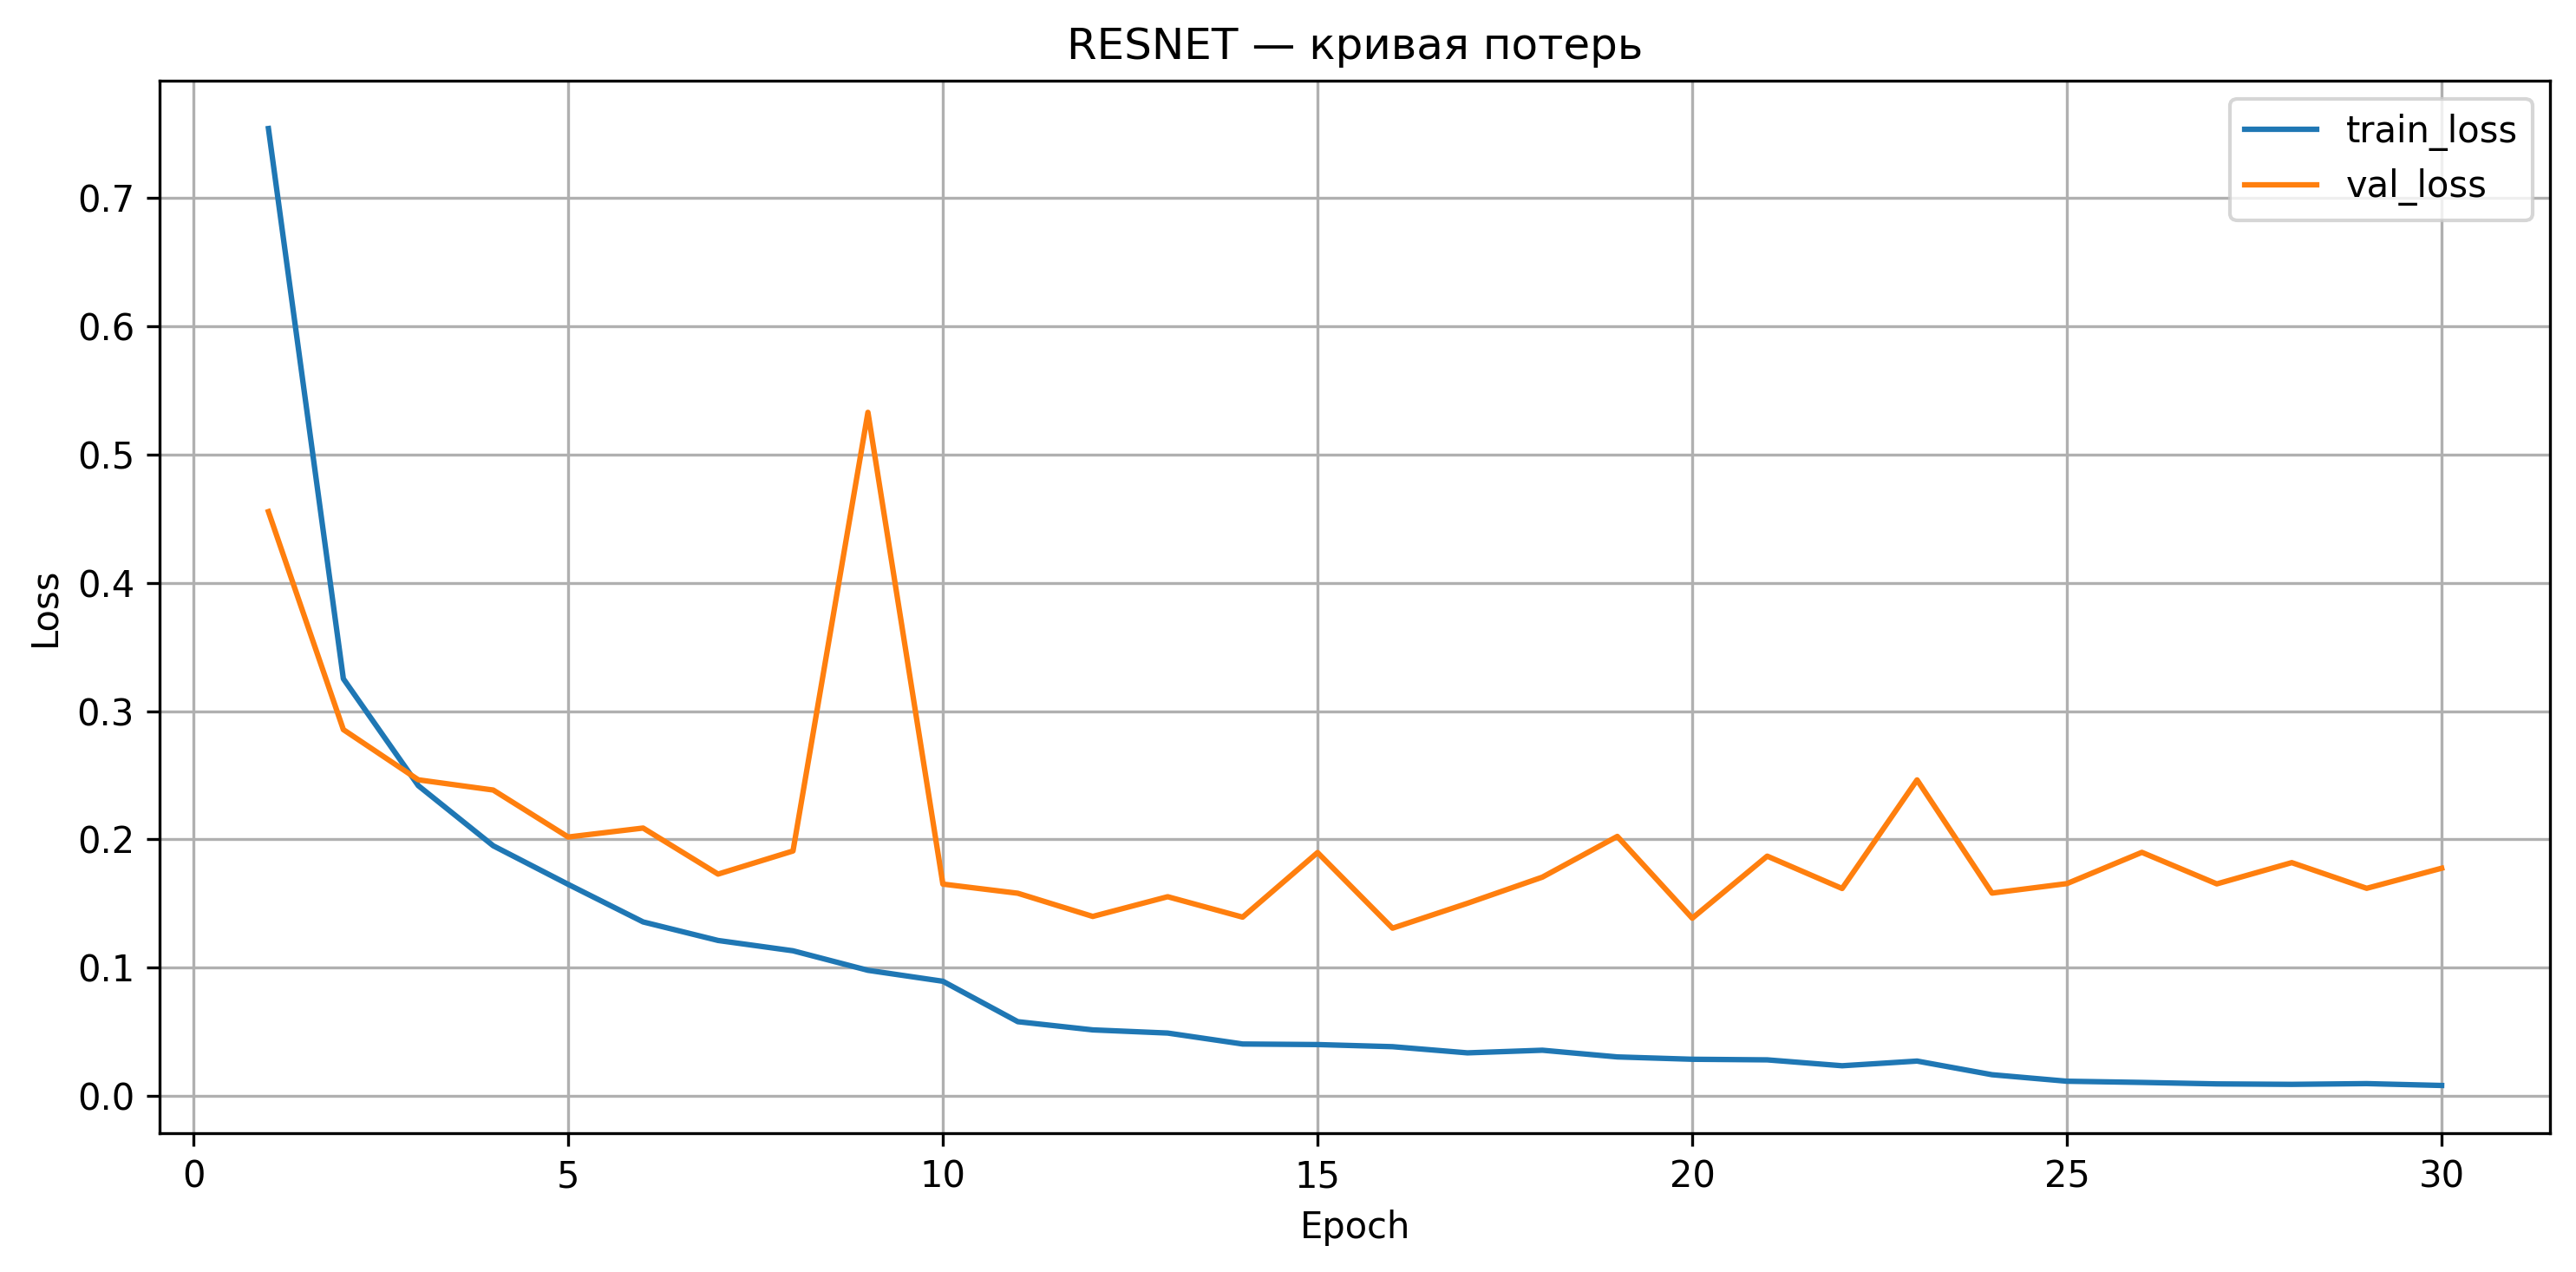
\includegraphics[width=\textwidth]{../reports/figures/models/resnet_loss_curve.png}
\end{minipage}
\hfill
\begin{minipage}{0.48\textwidth}
    \centering
    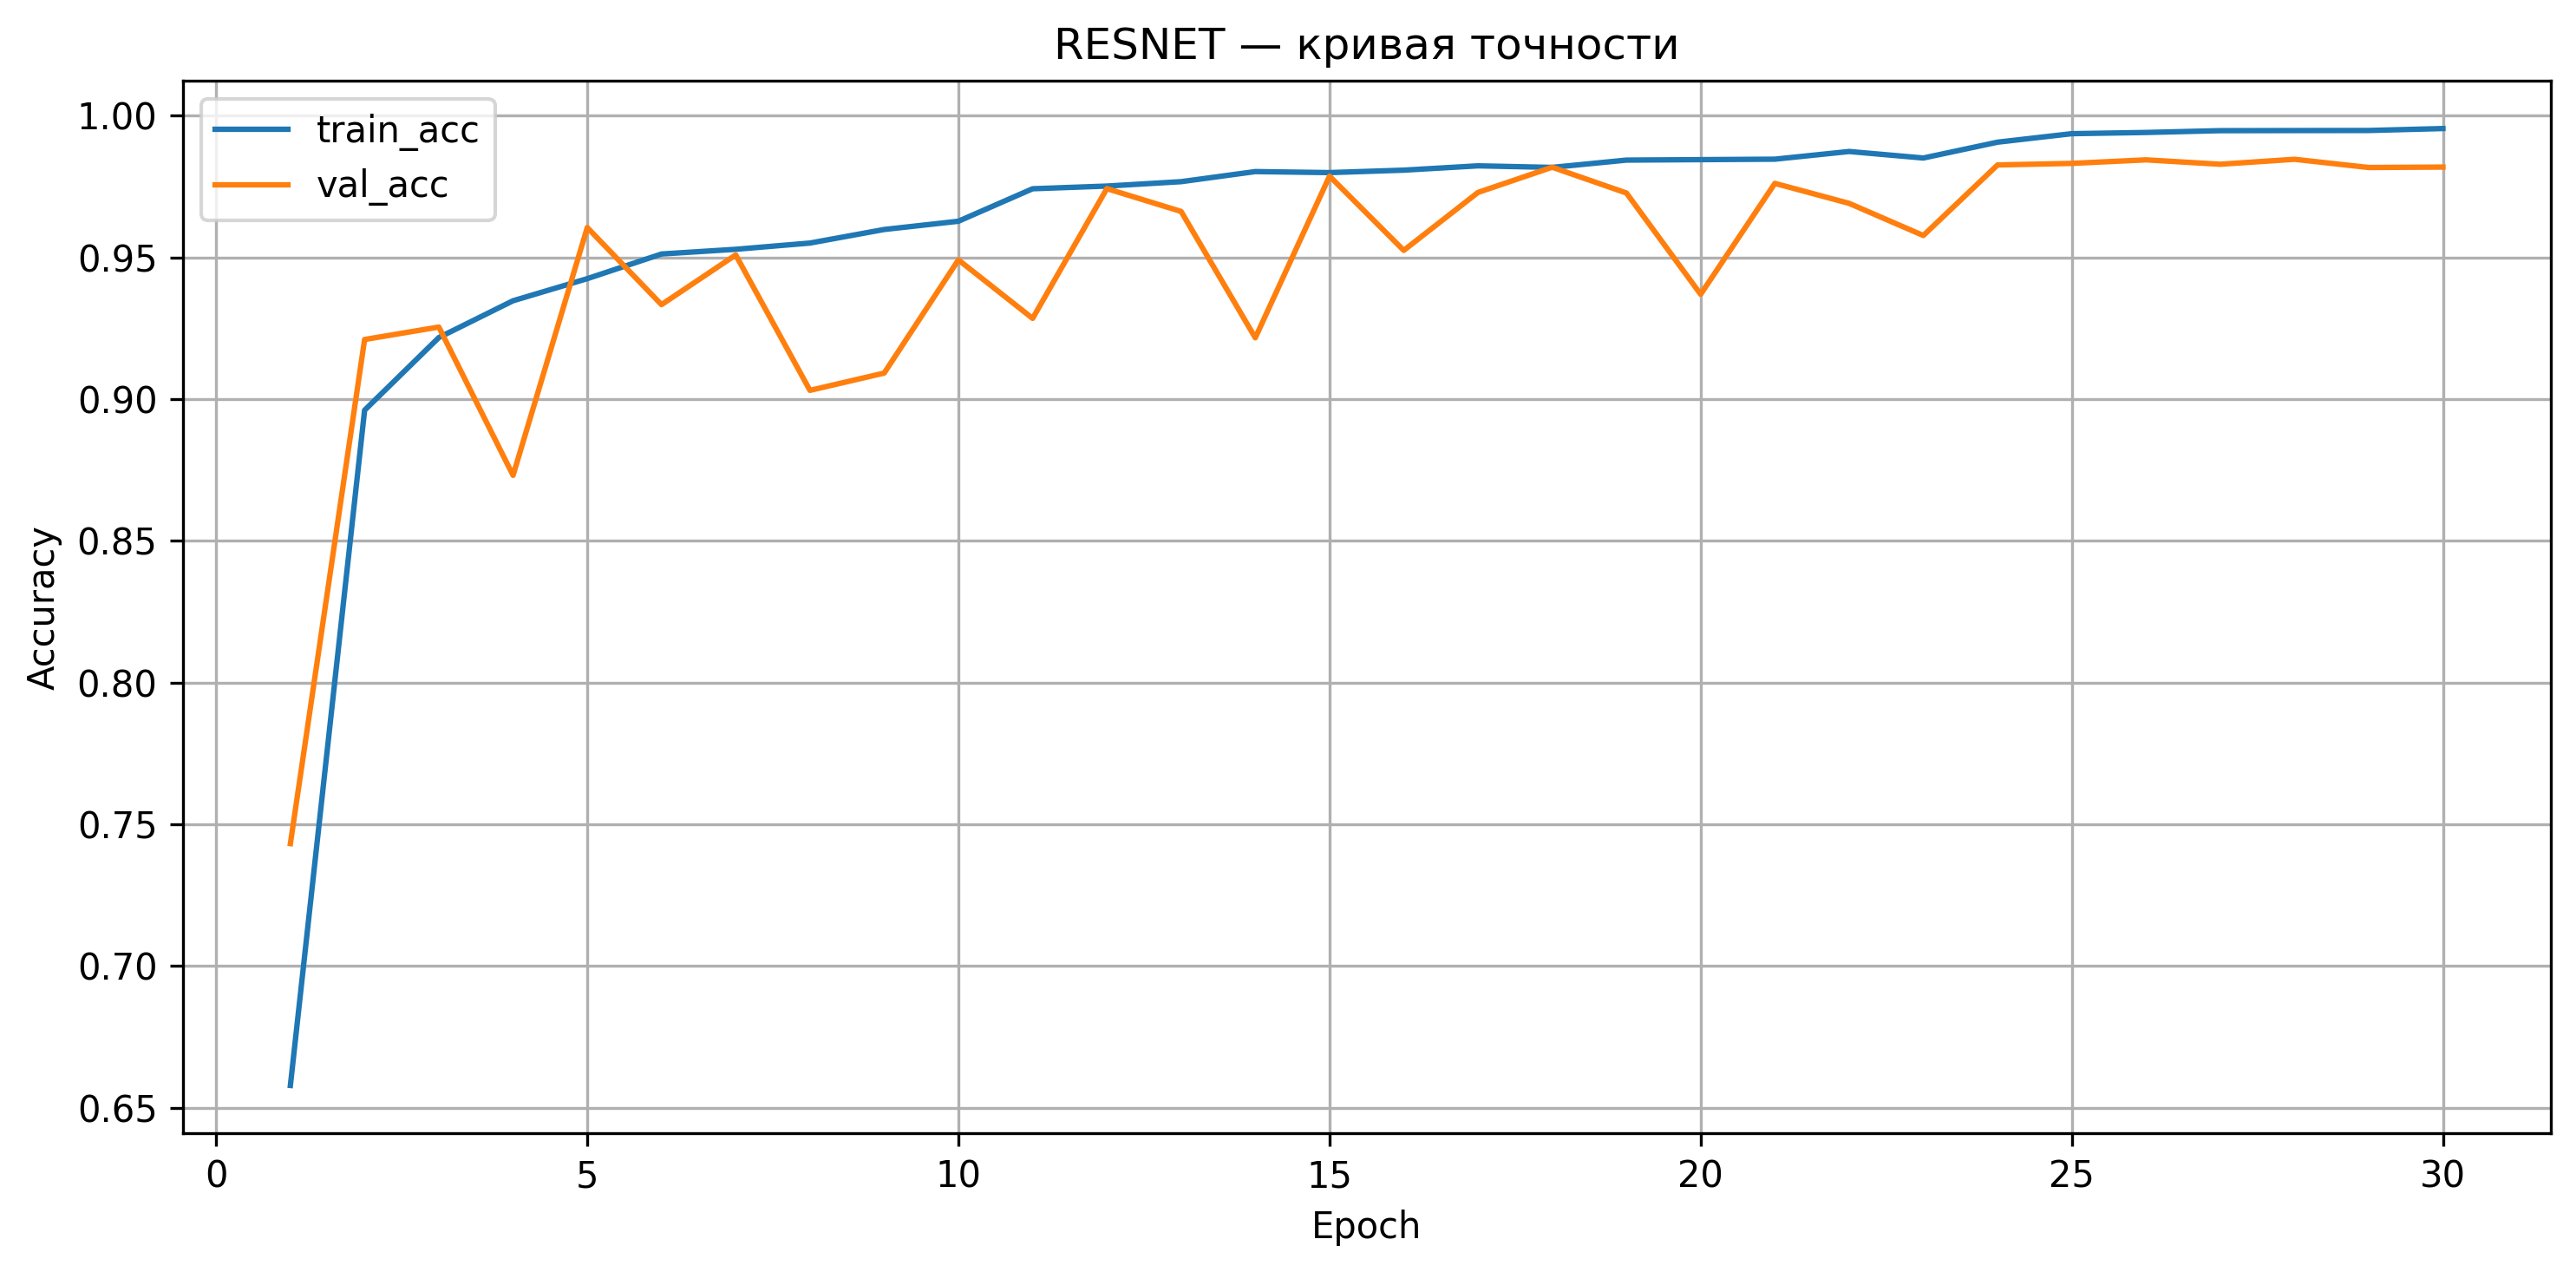
\includegraphics[width=\textwidth]{../reports/figures/models/resnet_accuracy_curve.png}
\end{minipage}
\caption{Кривые потерь и~точности ResNet1D.}
\label{fig:resnet_curves}
\end{figure}

ResNet1D требует больше эпох для~стабилизации по~сравнению
с~CNN, что~характерно для~более глубоких архитектур:
веса нескольких остаточных блоков должны согласоваться
друг~с~другом.
Остаточные соединения обеспечивают монотонное снижение потерь
без~«провалов», характерных для~сетей без~skip-connections.

\subsection{Важность признаков Random Forest}

\begin{figure}[h]
\centering
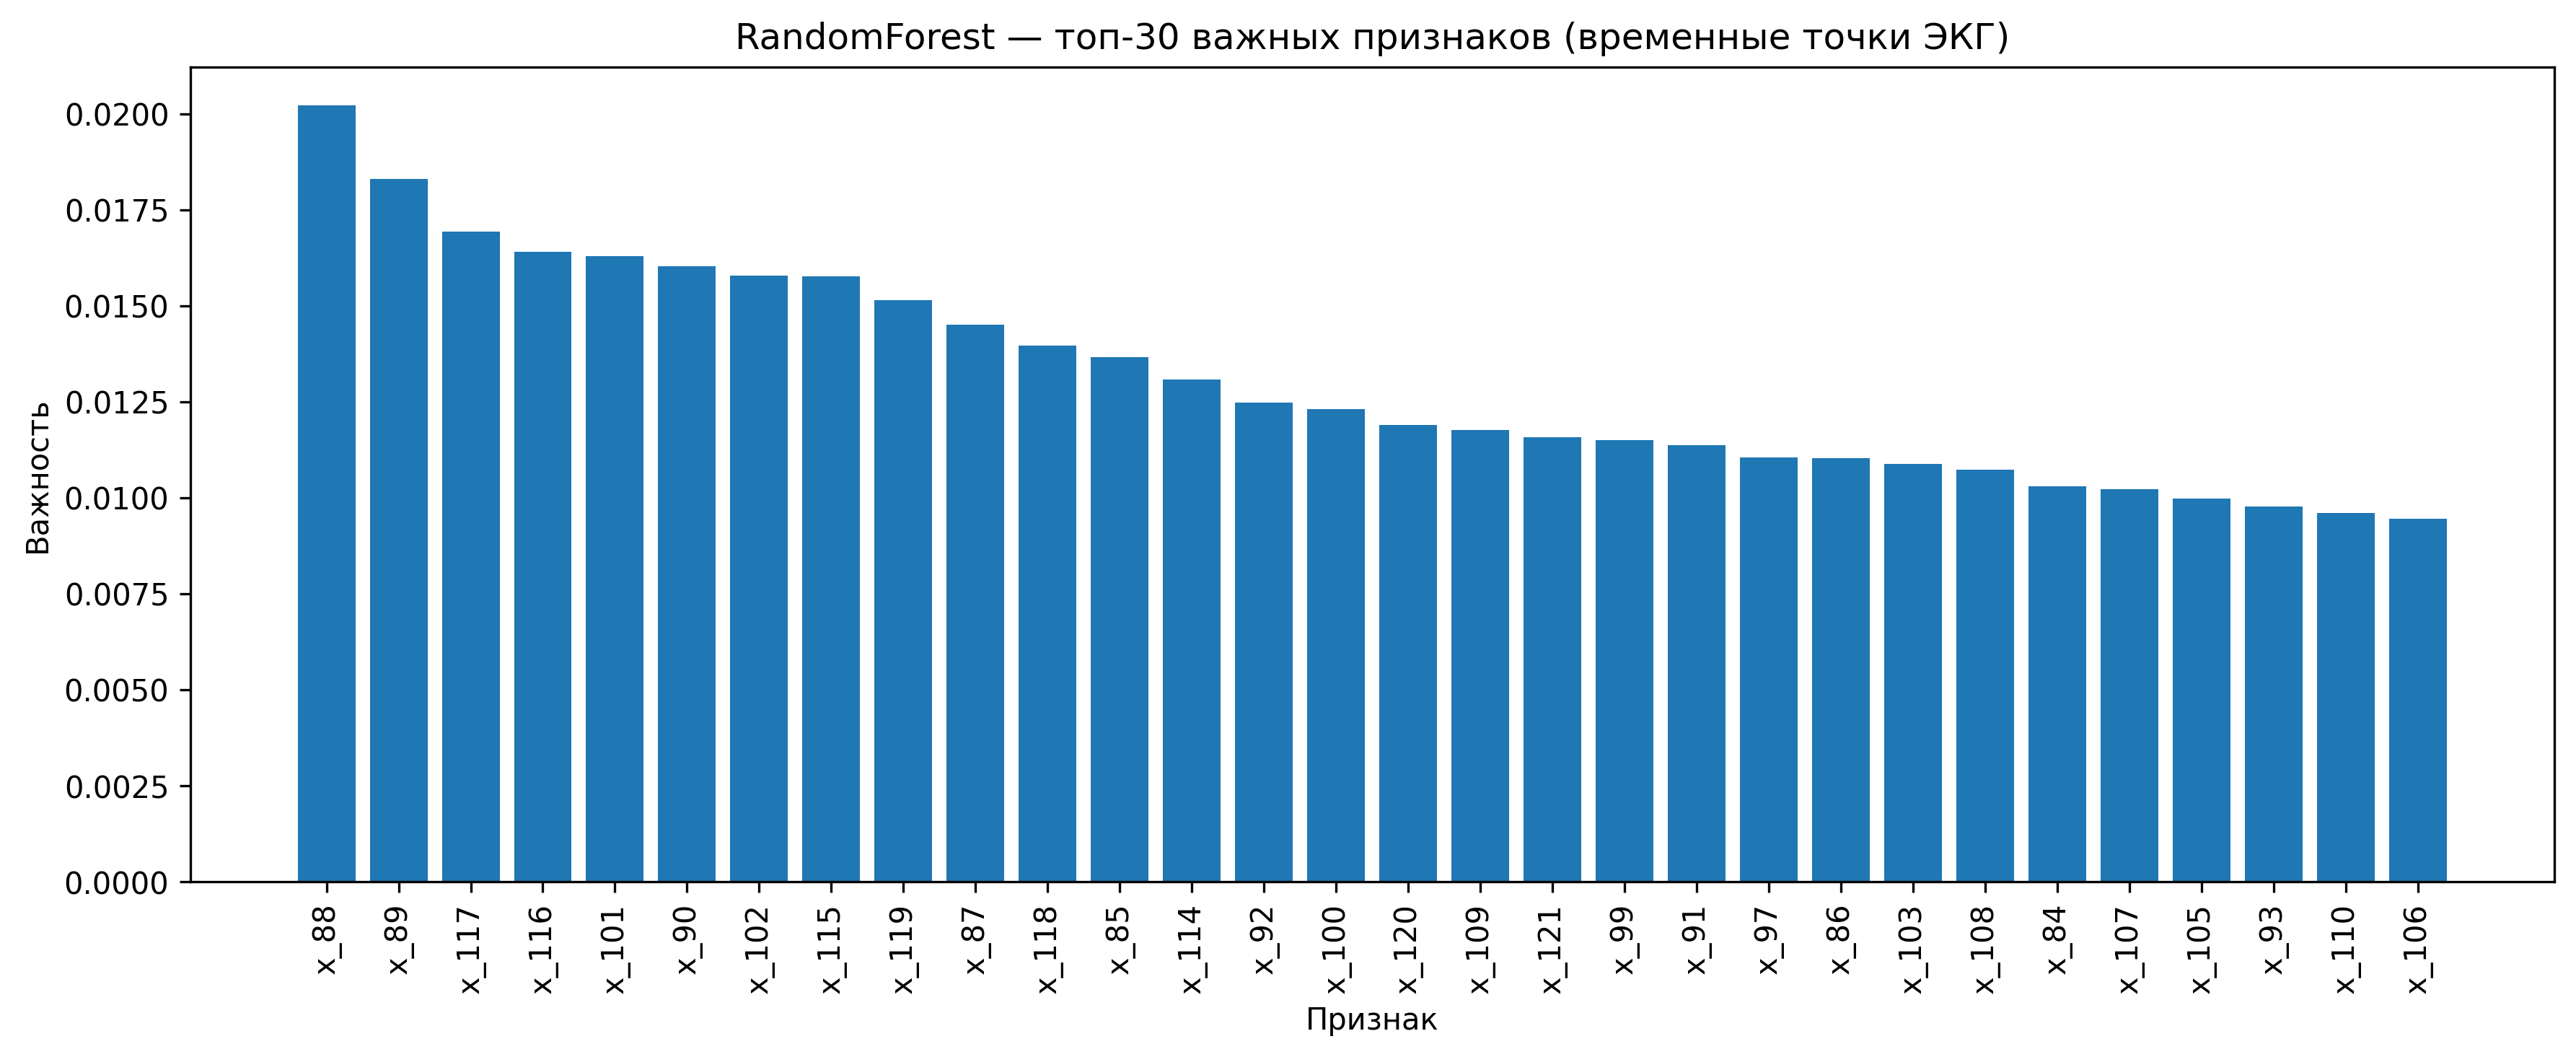
\includegraphics[width=\textwidth]{../reports/figures/models/rf_feature_importance.png}
\caption{Топ-30 наиболее важных временны\'{х} точек для~Random Forest
(оценка MDI).
По оси абсцисс~--- индекс отсчета в~окне $[x_0,\ldots,x_{239}]$;
по~оси ординат~--- нормированная важность.}
\label{fig:rf_importance}
\end{figure}

Наиболее информативными оказываются отсчеты в~диапазоне
$x_{95}$--$x_{115}$~--- непосредственно вблизи R-пика
(который находится в~позиции $x_{100}$).
Это соответствует крутому подъему и~спаду комплекса~QRS~---
наиболее характерному признаку для~разделения желудочковых
(V) и~предсердных (A) аномалий.
Отсчеты, соответствующие зубцу~T ($x_{140}$--$x_{200}$),
занимают второй по~значимости диапазон: форма~T-волны
дифференцирует блокады левой и~правой ножек (L~и~R).

\subsection{Эксперимент с вейвлет-признаками}

\begin{figure}[h]
\centering
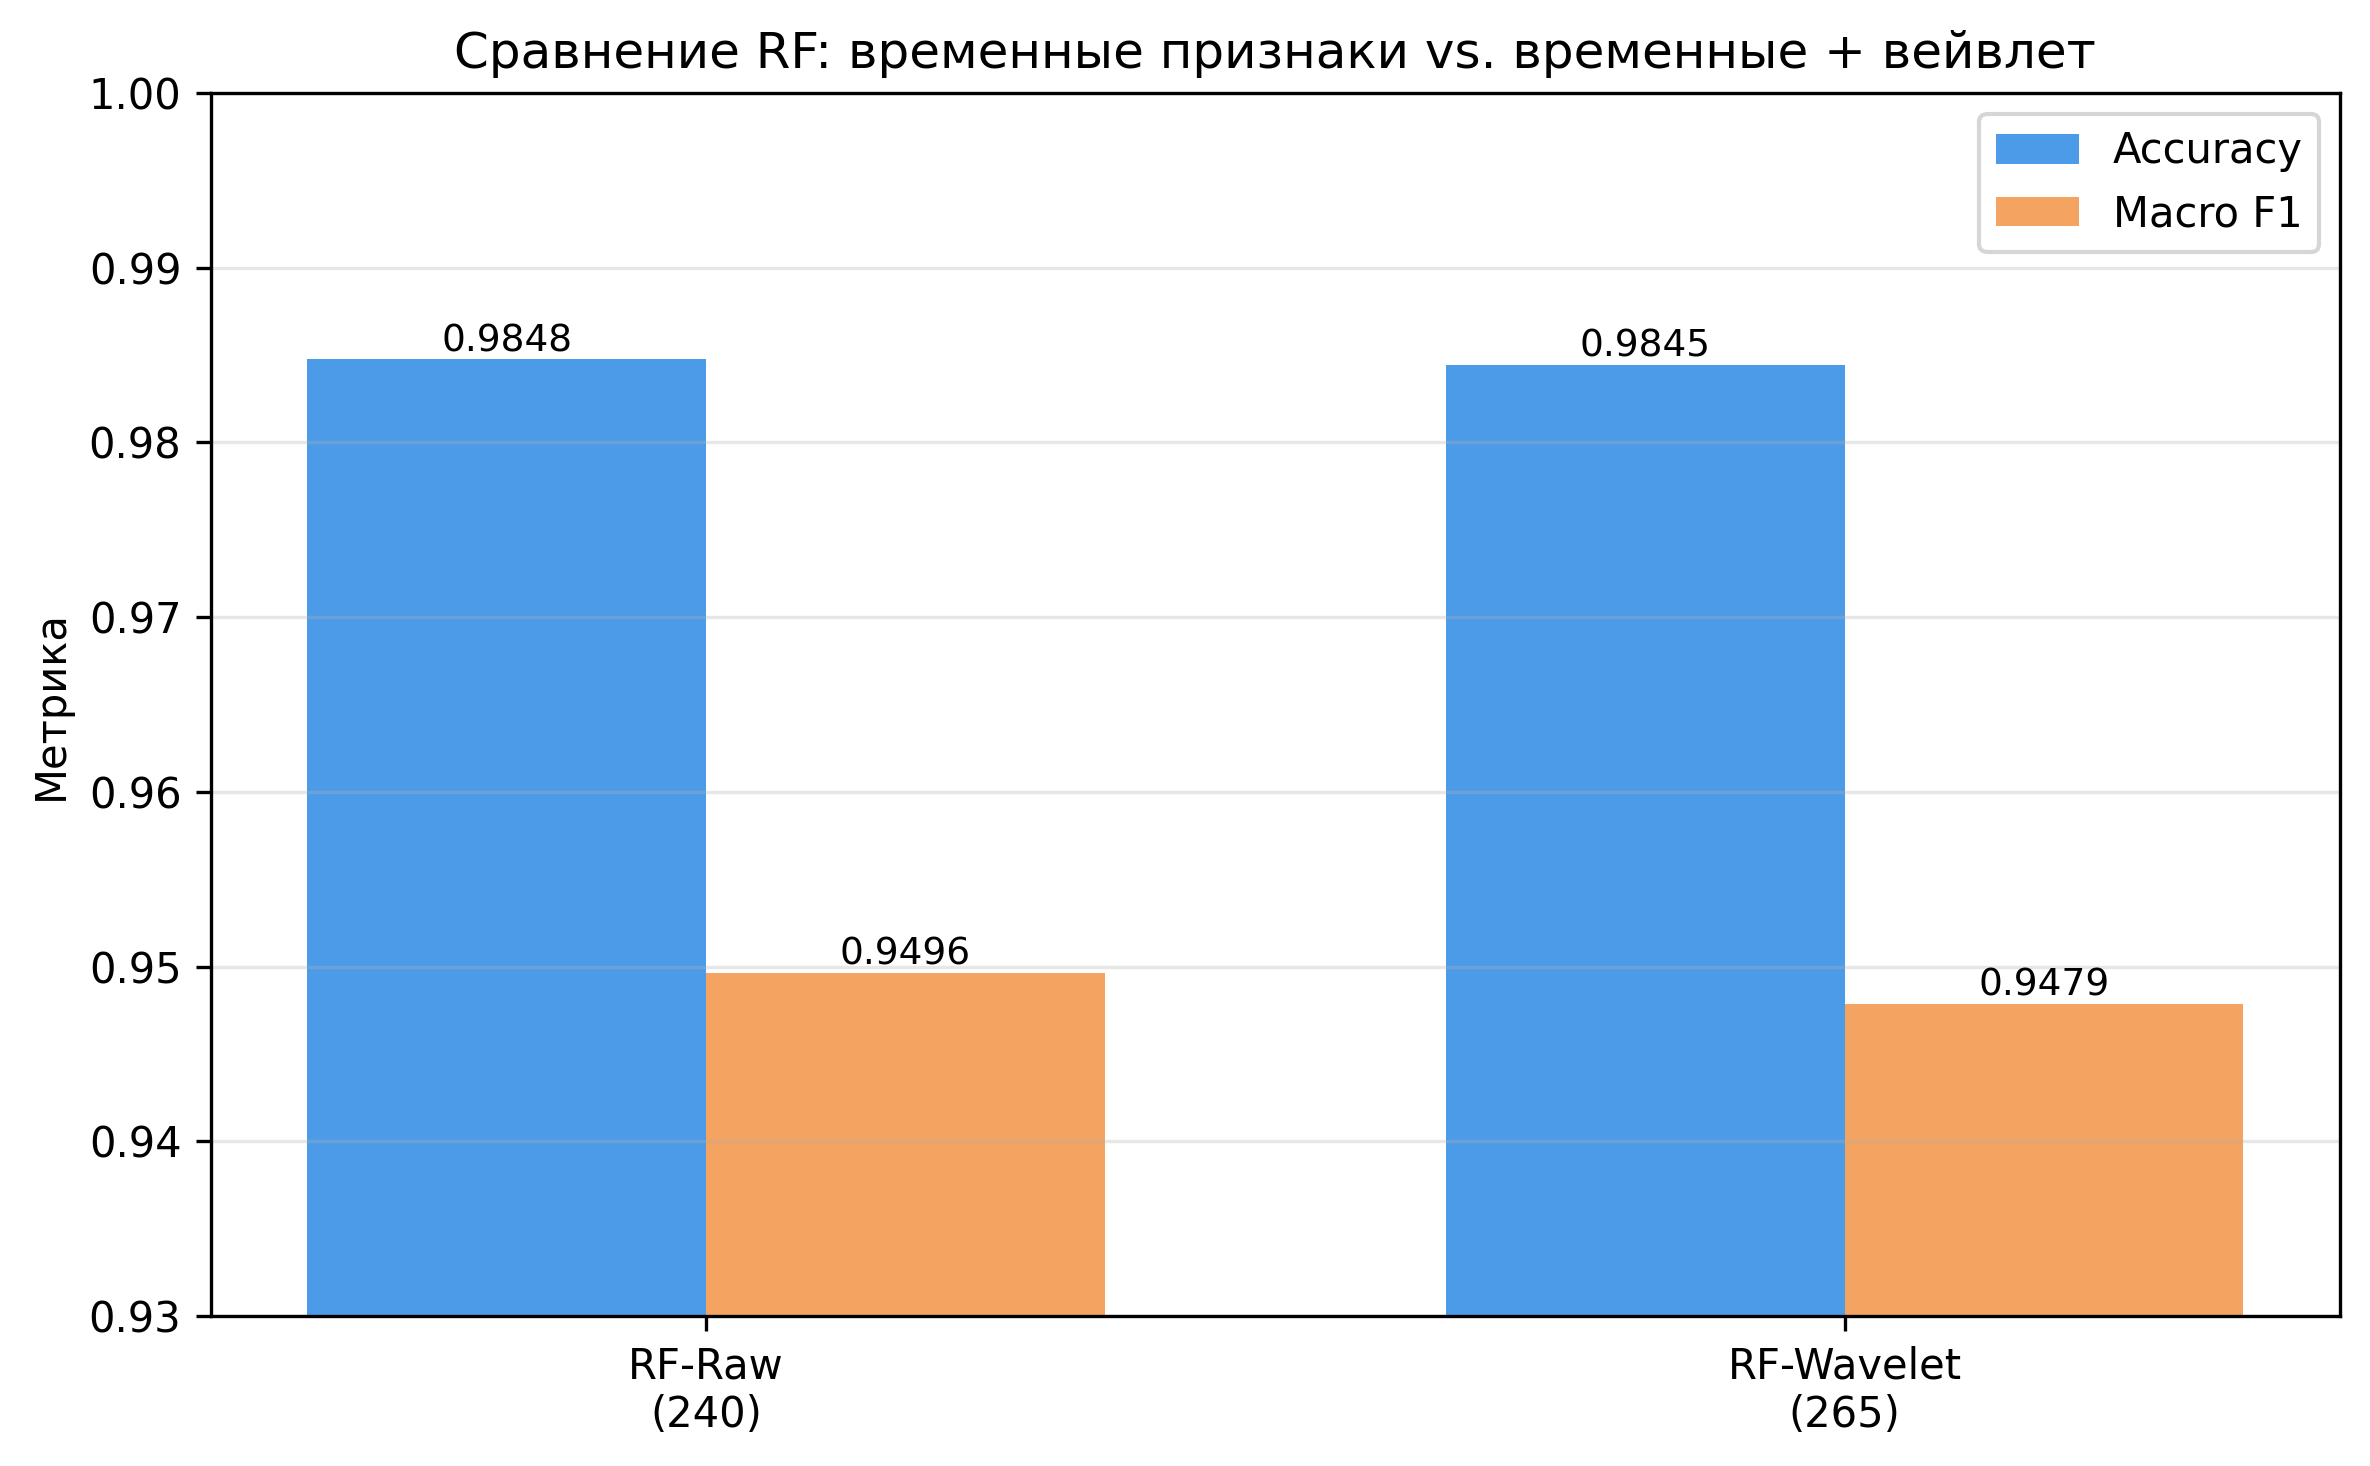
\includegraphics[width=0.75\textwidth]{../reports/figures/models/rf_wavelet_vs_raw_comparison.png}
\caption{Сравнение RF на~сырых признаках (240~отсчетов)
и~расширенных вейвлет-признаках (265~признаков).}
\label{fig:rf_wavelet_comp}
\end{figure}

Добавление $25$ вейвлет-признаков (ДВП db4, 4~уровня)
к~$240$ временны\'{м} отсчетам не~улучшило качество RF:
Macro~F1~$= 0.9479$ против~$0.9496$ (таблица~\ref{tab:wavelet_exp}).

\begin{table}[h]
\centering
\caption{Результаты эксперимента с вейвлет-признаками}
\label{tab:wavelet_exp}
\begin{tabular}{lcccc}
\hline
\textbf{Модель} & \textbf{Признаков} & \textbf{Accuracy} &
\textbf{Macro F1} & \textbf{Weighted F1} \\
\hline
RF-Raw     & 240 & 0.9848 & \textbf{0.9496} & 0.9841 \\
RF-Wavelet & 265 & 0.9845 & 0.9479          & 0.9837 \\
\hline
\end{tabular}
\end{table}

Разница Macro~F1~$= -0.0017$ находится в~пределах статистической
погрешности (для~выборки 20\,005~объектов оценка дисперсии
F1-меры невелика, однако систематического улучшения нет).
Вероятная причина: случайный лес на~$240$~сырых отсчетах
уже~неявно извлекает частотно-временны\'{е} паттерны~---
в~частности, разность соседних отсчетов кодирует локальную
производную, а~значит, и~высокочастотные компоненты.
Агрегатные статистики~($\bar{c},\,\sigma,\,E$) по~каждой
подполосе, напротив, теряют позиционную информацию.

Важность групп признаков (рисунок~\ref{fig:wt_imp}) показывает,
что~суммарный вклад $240$ временны\'{х} точек значительно
превышает суммарный вклад всех $25$ вейвлет-признаков.
Среди вейвлет-подполос наибольший вклад вносят $\mathrm{cD}_3$
и~$\mathrm{cD}_4$, соответствующие диапазону $11$--$45$~Гц,~---
именно там сосредоточена энергия комплекса~QRS и~зубцов~P, T.

\begin{figure}[h]
\centering
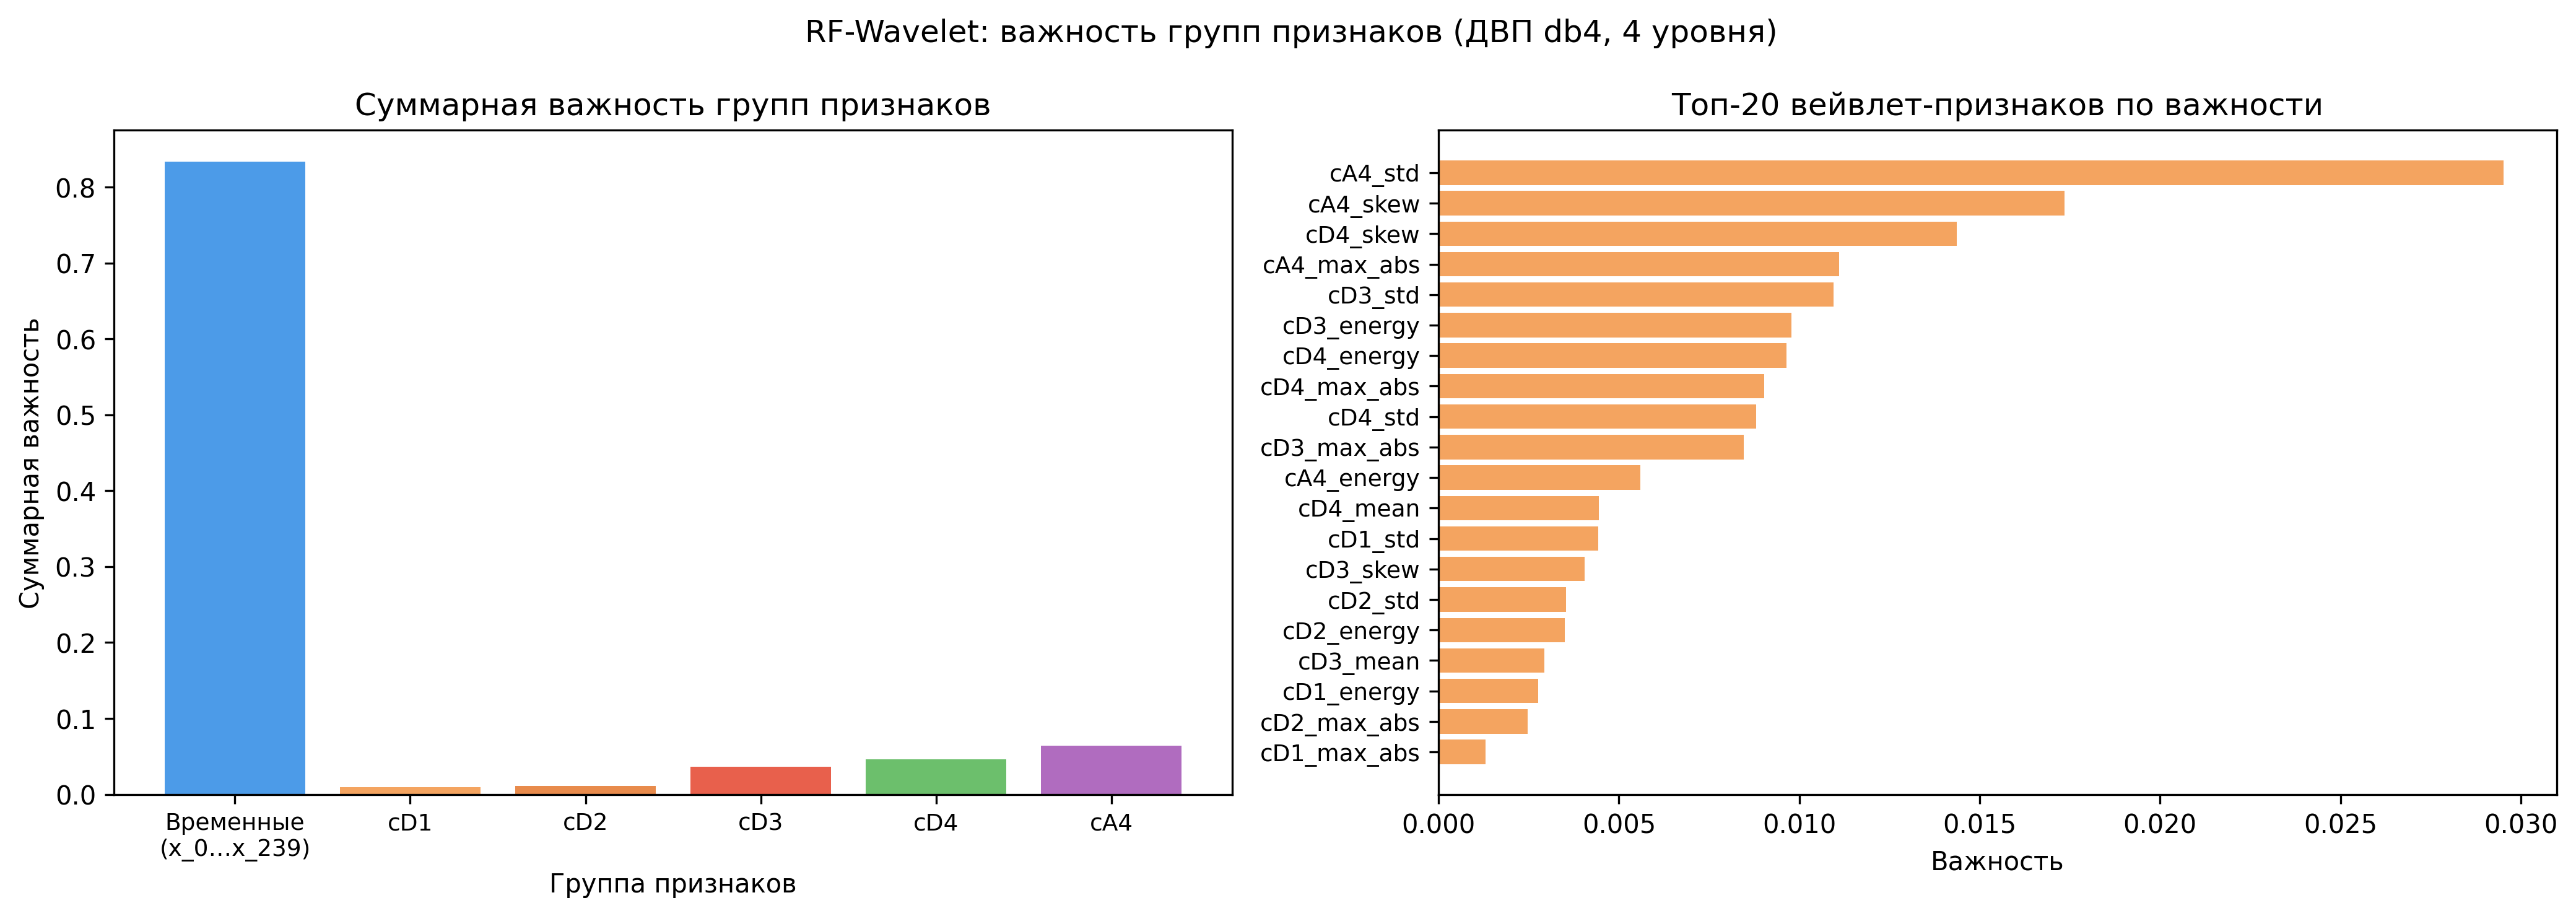
\includegraphics[width=\textwidth]{../reports/figures/models/rf_wavelet_feature_importance.png}
\caption{Важность групп признаков в~RF-Wavelet (слева~---
суммарно по~группам, справа~--- топ-20 вейвлет-признаков).}
\label{fig:wt_imp}
\end{figure}
 % Результаты на чистых данных
\section{Устойчивость к шуму и кросс-валидация}
\label{sec:Chapter4}

\subsection{Модели артефактов ЭКГ-сигналов}

В~реальных условиях холтеровского мониторирования запись ЭКГ
неизбежно содержит артефакты различной природы.
В~работе рассматриваются четыре типа помех, наиболее типичных
при~амбулаторной регистрации.

\paragraph{Гауссов шум.}
Моделирует тепловые и~квантовые шумы усилительного тракта:
\begin{equation}
    \tilde{s}[n] = s[n] + \varepsilon[n],\quad
    \varepsilon[n] \sim \mathcal{N}(0,\,\sigma^2).
\end{equation}
Уровень шума характеризуется параметром $\sigma$ и~нарастает
от~$0.01$ до~$0.08$~мВ с~шагом~$0.01$.

\paragraph{Дрейф изолинии.}
Вызван дыхательными движениями и~нестабильным контактом
электрода с~кожей; аппроксимируется медленной синусоидой:
\begin{equation}
    \tilde{s}[n] = s[n] + A\sin\!\left(\frac{2\pi f_0 n}{f_s}\right),
    \quad f_0 = 0.5\;\text{Гц}.
\end{equation}
Амплитуда $A$ варьируется от~$0.01$ до~$0.15$~мВ с~шагом~$0.01$.

\paragraph{Сетевая помеха~50~Гц.}
Индуктивная наводка от~сети электропитания:
\begin{equation}
    \tilde{s}[n] = s[n] + A\sin\!\left(\frac{2\pi \cdot 50 \cdot n}{f_s}\right).
\end{equation}
Амплитуда $A$~--- от~$0.01$ до~$0.08$~мВ.

\paragraph{Мышечный шум~(ЭМГ).}
Сигнал скелетных мышц накладывается на~ЭКГ при~физической
активности; моделируется сглаженным гауссовым шумом:
\begin{equation}
    \tilde{s}[n] = s[n] + (A \cdot \varepsilon) * h[n],
\end{equation}
где $\varepsilon \sim \mathcal{N}(0,1)$, $h[n]$~--- прямоугольный
сглаживающий фильтр длиной~$5$~отсчетов.
Амплитуда $A$~--- от~$0.01$ до~$0.07$~мВ.

\subsection{Результаты экспериментов с шумом}

Для~каждого типа и~уровня помехи вычислялись Accuracy и~Macro~F1
всех~трех моделей на~тестовой выборке~($20\,005$~объектов).
Сводные результаты при~максимальных уровнях помех
приведены в~таблице~\ref{tab:noise_max}.

\begin{table}[h]
\centering
\caption{Метрики при максимальных уровнях шума}
\label{tab:noise_max}
\begin{tabular}{llccc}
\hline
\textbf{Тип шума} & \textbf{Уровень} & \textbf{Модель} &
\textbf{Accuracy} & \textbf{Macro F1} \\
\hline
\multirow{3}{*}{Гауссов шум}      & \multirow{3}{*}{$\sigma{=}0.08$}
  & CNN         & 0.9446 & 0.7869 \\
& & ResNet1D    & 0.8619 & 0.5888 \\
& & RandomForest & \textbf{0.9703} & \textbf{0.8716} \\
\hline
\multirow{3}{*}{Дрейф изолинии}   & \multirow{3}{*}{$A{=}0.15$}
  & CNN         & \textbf{0.9918} & \textbf{0.9740} \\
& & ResNet1D    & 0.9833 & 0.9498 \\
& & RandomForest & 0.9719 & 0.8901 \\
\hline
\multirow{3}{*}{Сетевая помеха}   & \multirow{3}{*}{$A{=}0.08$}
  & CNN         & 0.9832 & 0.9357 \\
& & ResNet1D    & 0.8427 & 0.6395 \\
& & RandomForest & \textbf{0.9767} & \textbf{0.9114} \\
\hline
\multirow{3}{*}{Мышечный шум}     & \multirow{3}{*}{$A{=}0.07$}
  & CNN         & \textbf{0.9882} & \textbf{0.9603} \\
& & ResNet1D    & 0.9758 & 0.9228 \\
& & RandomForest & 0.9830 & 0.9422 \\
\hline
\end{tabular}
\end{table}

\subsubsection{Гауссов шум}

\begin{figure}[h]
\centering
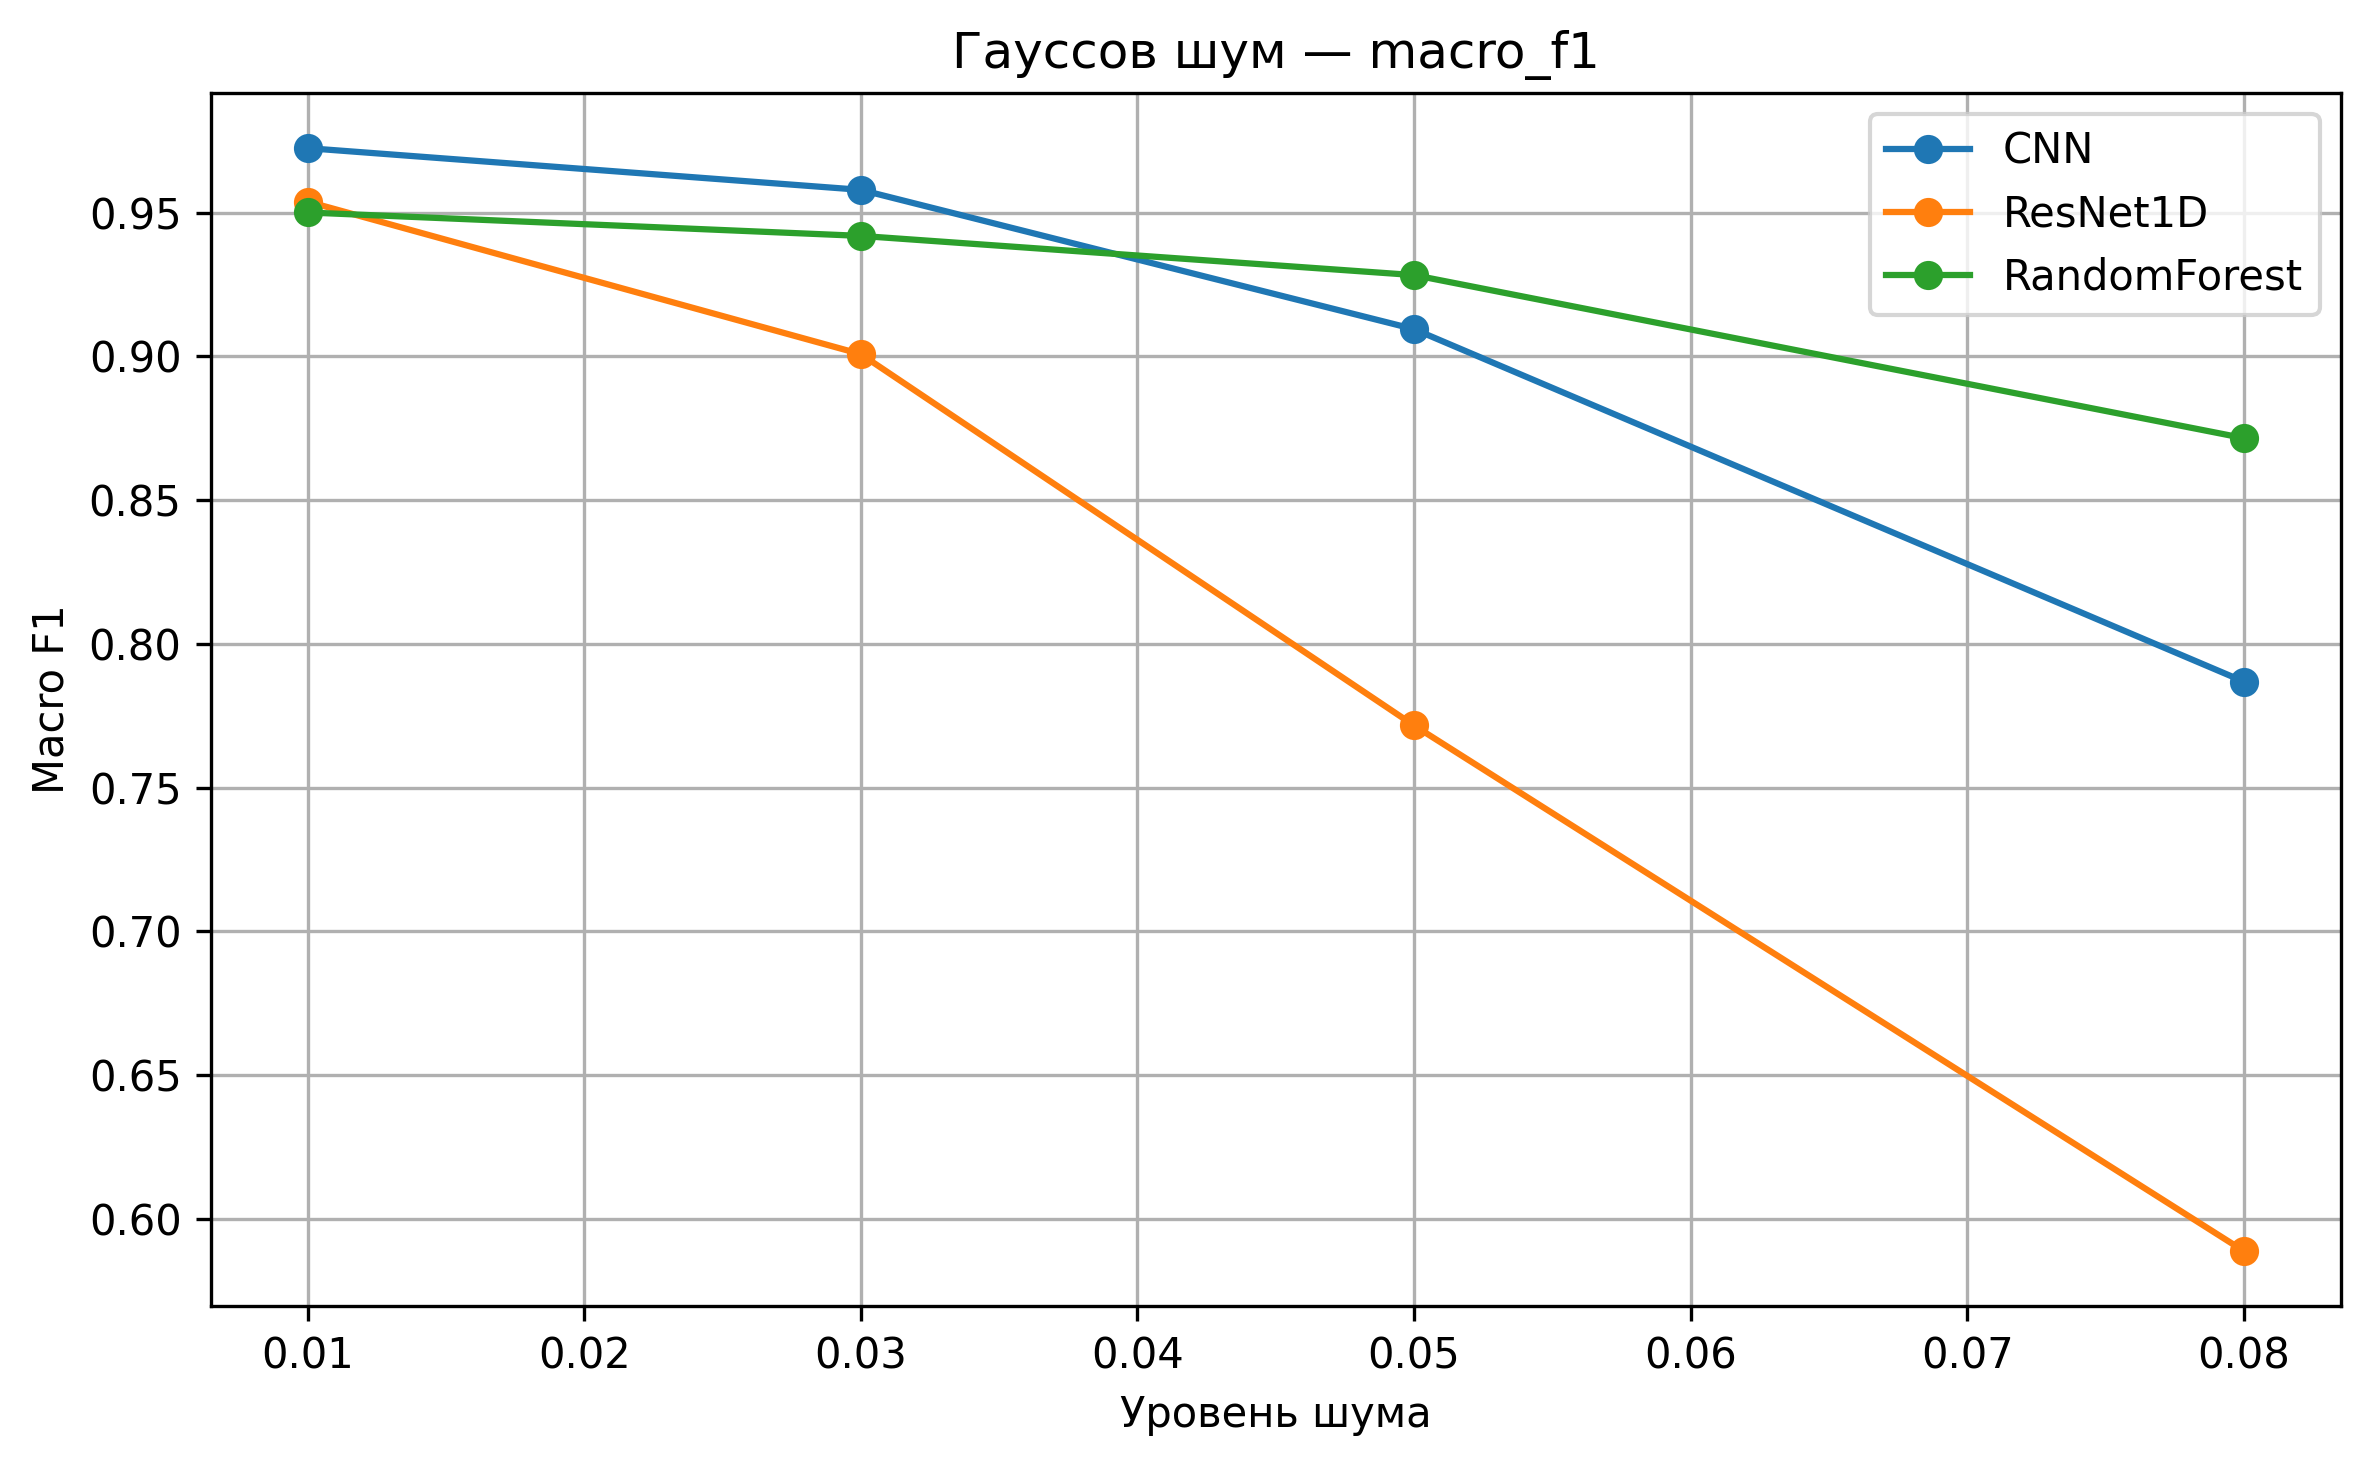
\includegraphics[width=0.85\textwidth]{../reports/figures/models/noise_gaussian_macro_f1.png}
\caption{Зависимость Macro~F1 от~уровня гауссова шума~$\sigma$.}
\label{fig:noise_gaussian}
\end{figure}

При~$\sigma = 0.08$~мВ случайный лес сохраняет Macro~F1~$= 0.872$,
тогда~как~CNN опускается до~$0.787$, а~ResNet1D~--- до~$0.589$.
RF устойчив к~случайным аддитивным помехам: пороговые разбиения
деревьев не~чувствительны к~равномерно распределенному по~спектру
шуму, который усредняется при~нахождении оптимального порога.
CNN теряет точность сильнее: сверточные фильтры обнаруживают
высокочастотные компоненты QRS, которые при~высоком $\sigma$
«маскируются» шумом.

\subsubsection{Дрейф изолинии}

\begin{figure}[h]
\centering
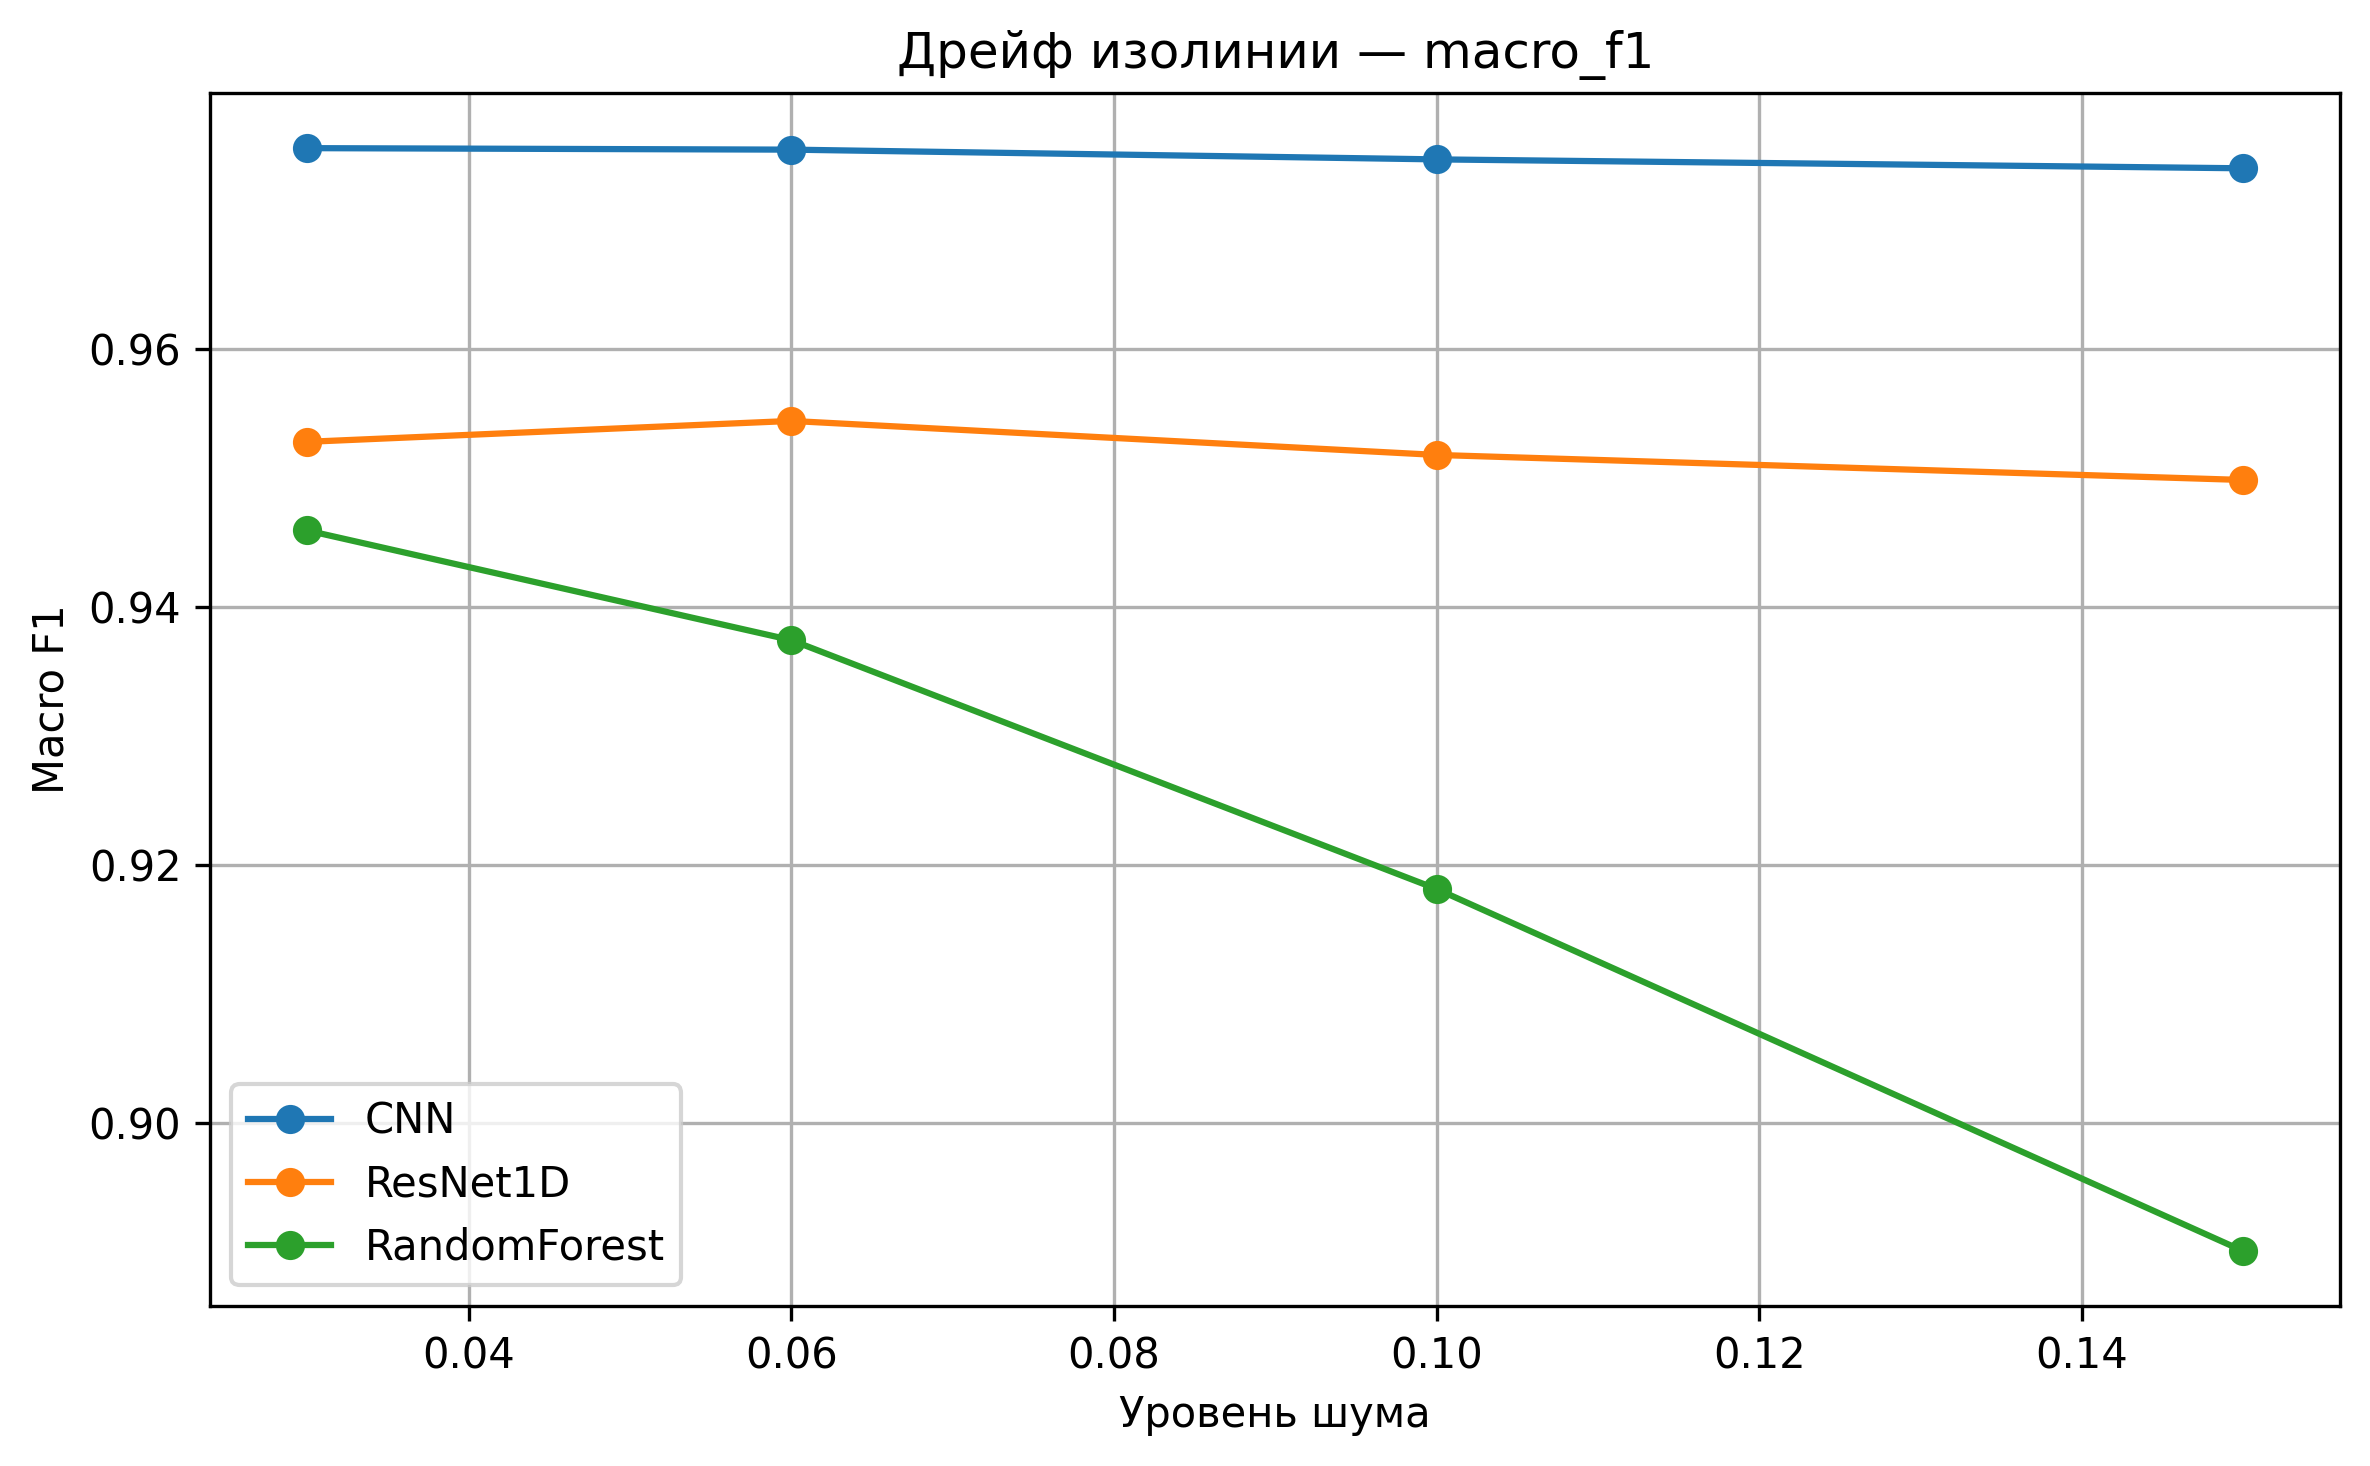
\includegraphics[width=0.85\textwidth]{../reports/figures/models/noise_baseline_macro_f1.png}
\caption{Зависимость Macro~F1 от~амплитуды дрейфа изолинии~$A$.}
\label{fig:noise_baseline}
\end{figure}

Наиболее устойчивой к~дрейфу оказалась CNN:
Macro~F1~$= 0.974$ при~$A = 0.15$~мВ~--- практически без~потерь
относительно чистых данных.
Причина~--- BatchNorm внутри сверточных блоков нормализует
активации по~мини-батчу, фактически компенсируя медленное
смещение изолинии.
ResNet1D также устойчив ($0.950$).
RF деградирует сильнее ($0.890$): деревья строят пороги
по~абсолютным значениям отсчетов и~чувствительны к~сдвигу
постоянной составляющей.

\subsubsection{Сетевая помеха 50~Гц}

\begin{figure}[h]
\centering
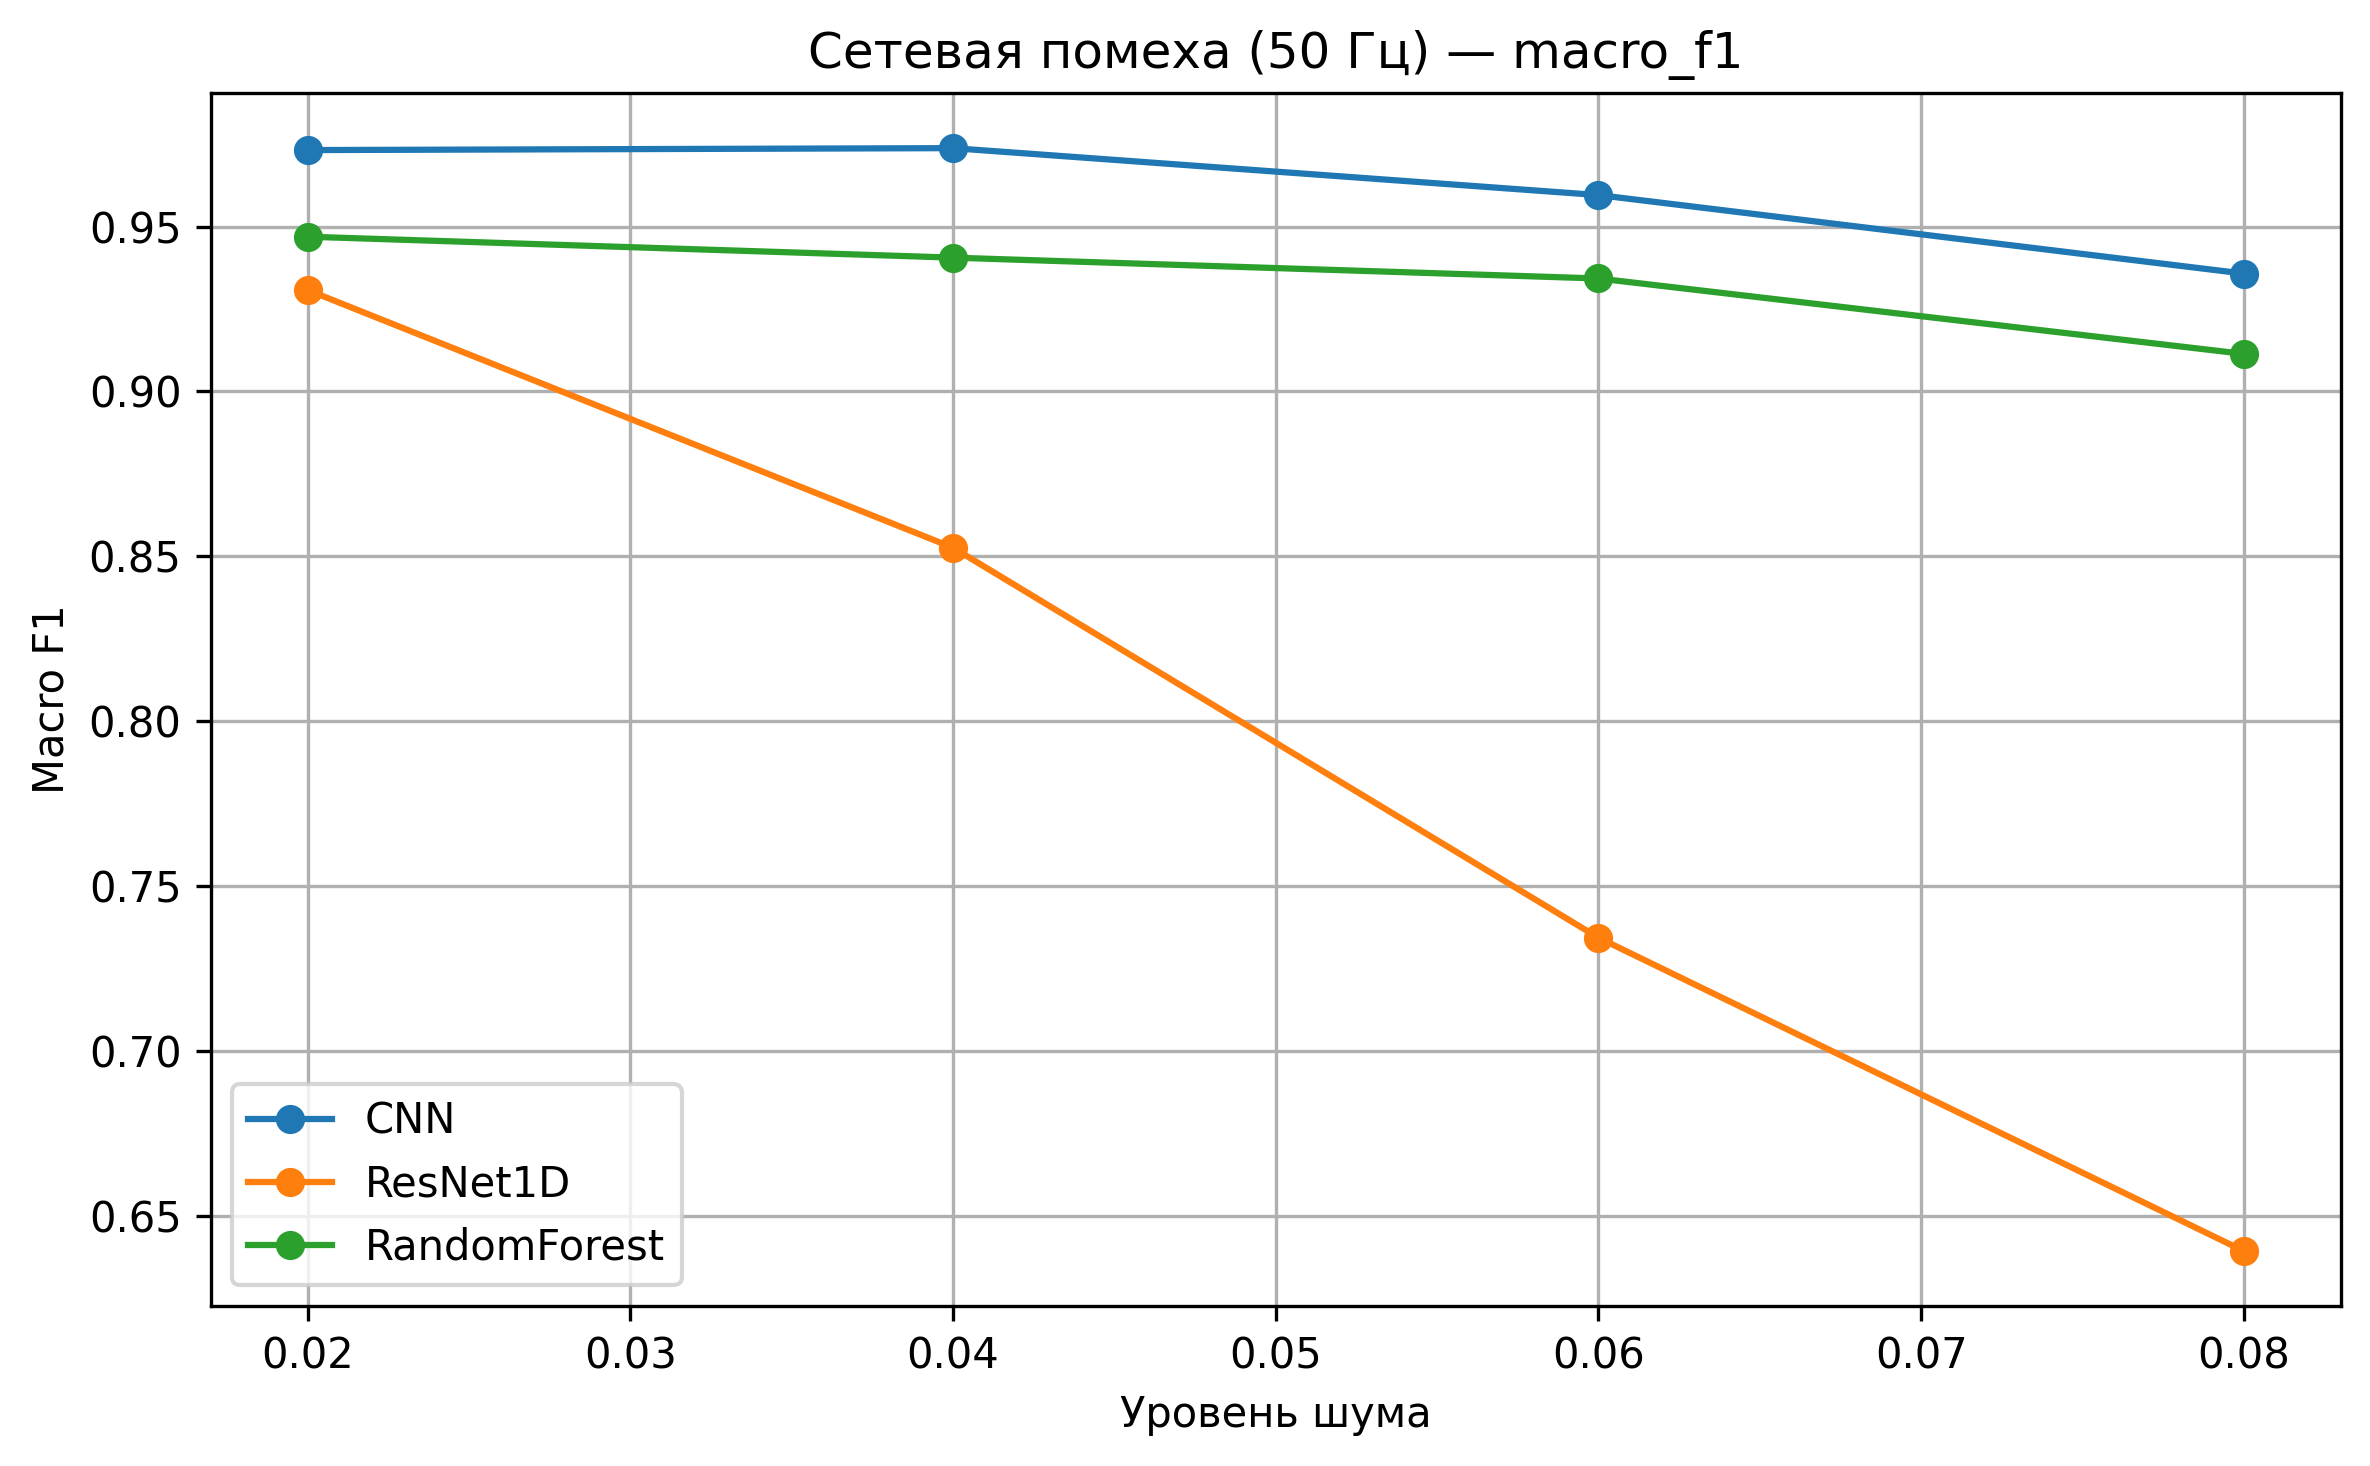
\includegraphics[width=0.85\textwidth]{../reports/figures/models/noise_powerline_macro_f1.png}
\caption{Зависимость Macro~F1 от~амплитуды сетевой помехи~50~Гц.}
\label{fig:noise_powerline}
\end{figure}

Сетевая помеха особенно разрушительна для~ResNet1D:
Macro~F1~падает до~$0.640$~--- потеря $0.31$ относительно
чистых данных.
Слой \texttt{AdaptiveAvgPool1d(1)} глобально усредняет карту
признаков по~временному измерению: периодическая синусоида
частотой~$50$~Гц ($\lambda \approx 7.2$~отсчета) создает
регулярные паттерны, которые после~усреднения дают ненулевые
сдвиги в~признаковом пространстве.
CNN устойчивее ($0.936$): два уровня MaxPool перед
AdaptiveAvgPool частично подавляют высокочастотные компоненты.
RF стабилен ($0.911$): пороговые деления нечувствительны
к~периодическим помехам средней амплитуды.

\subsubsection{Мышечный шум}

\begin{figure}[h]
\centering
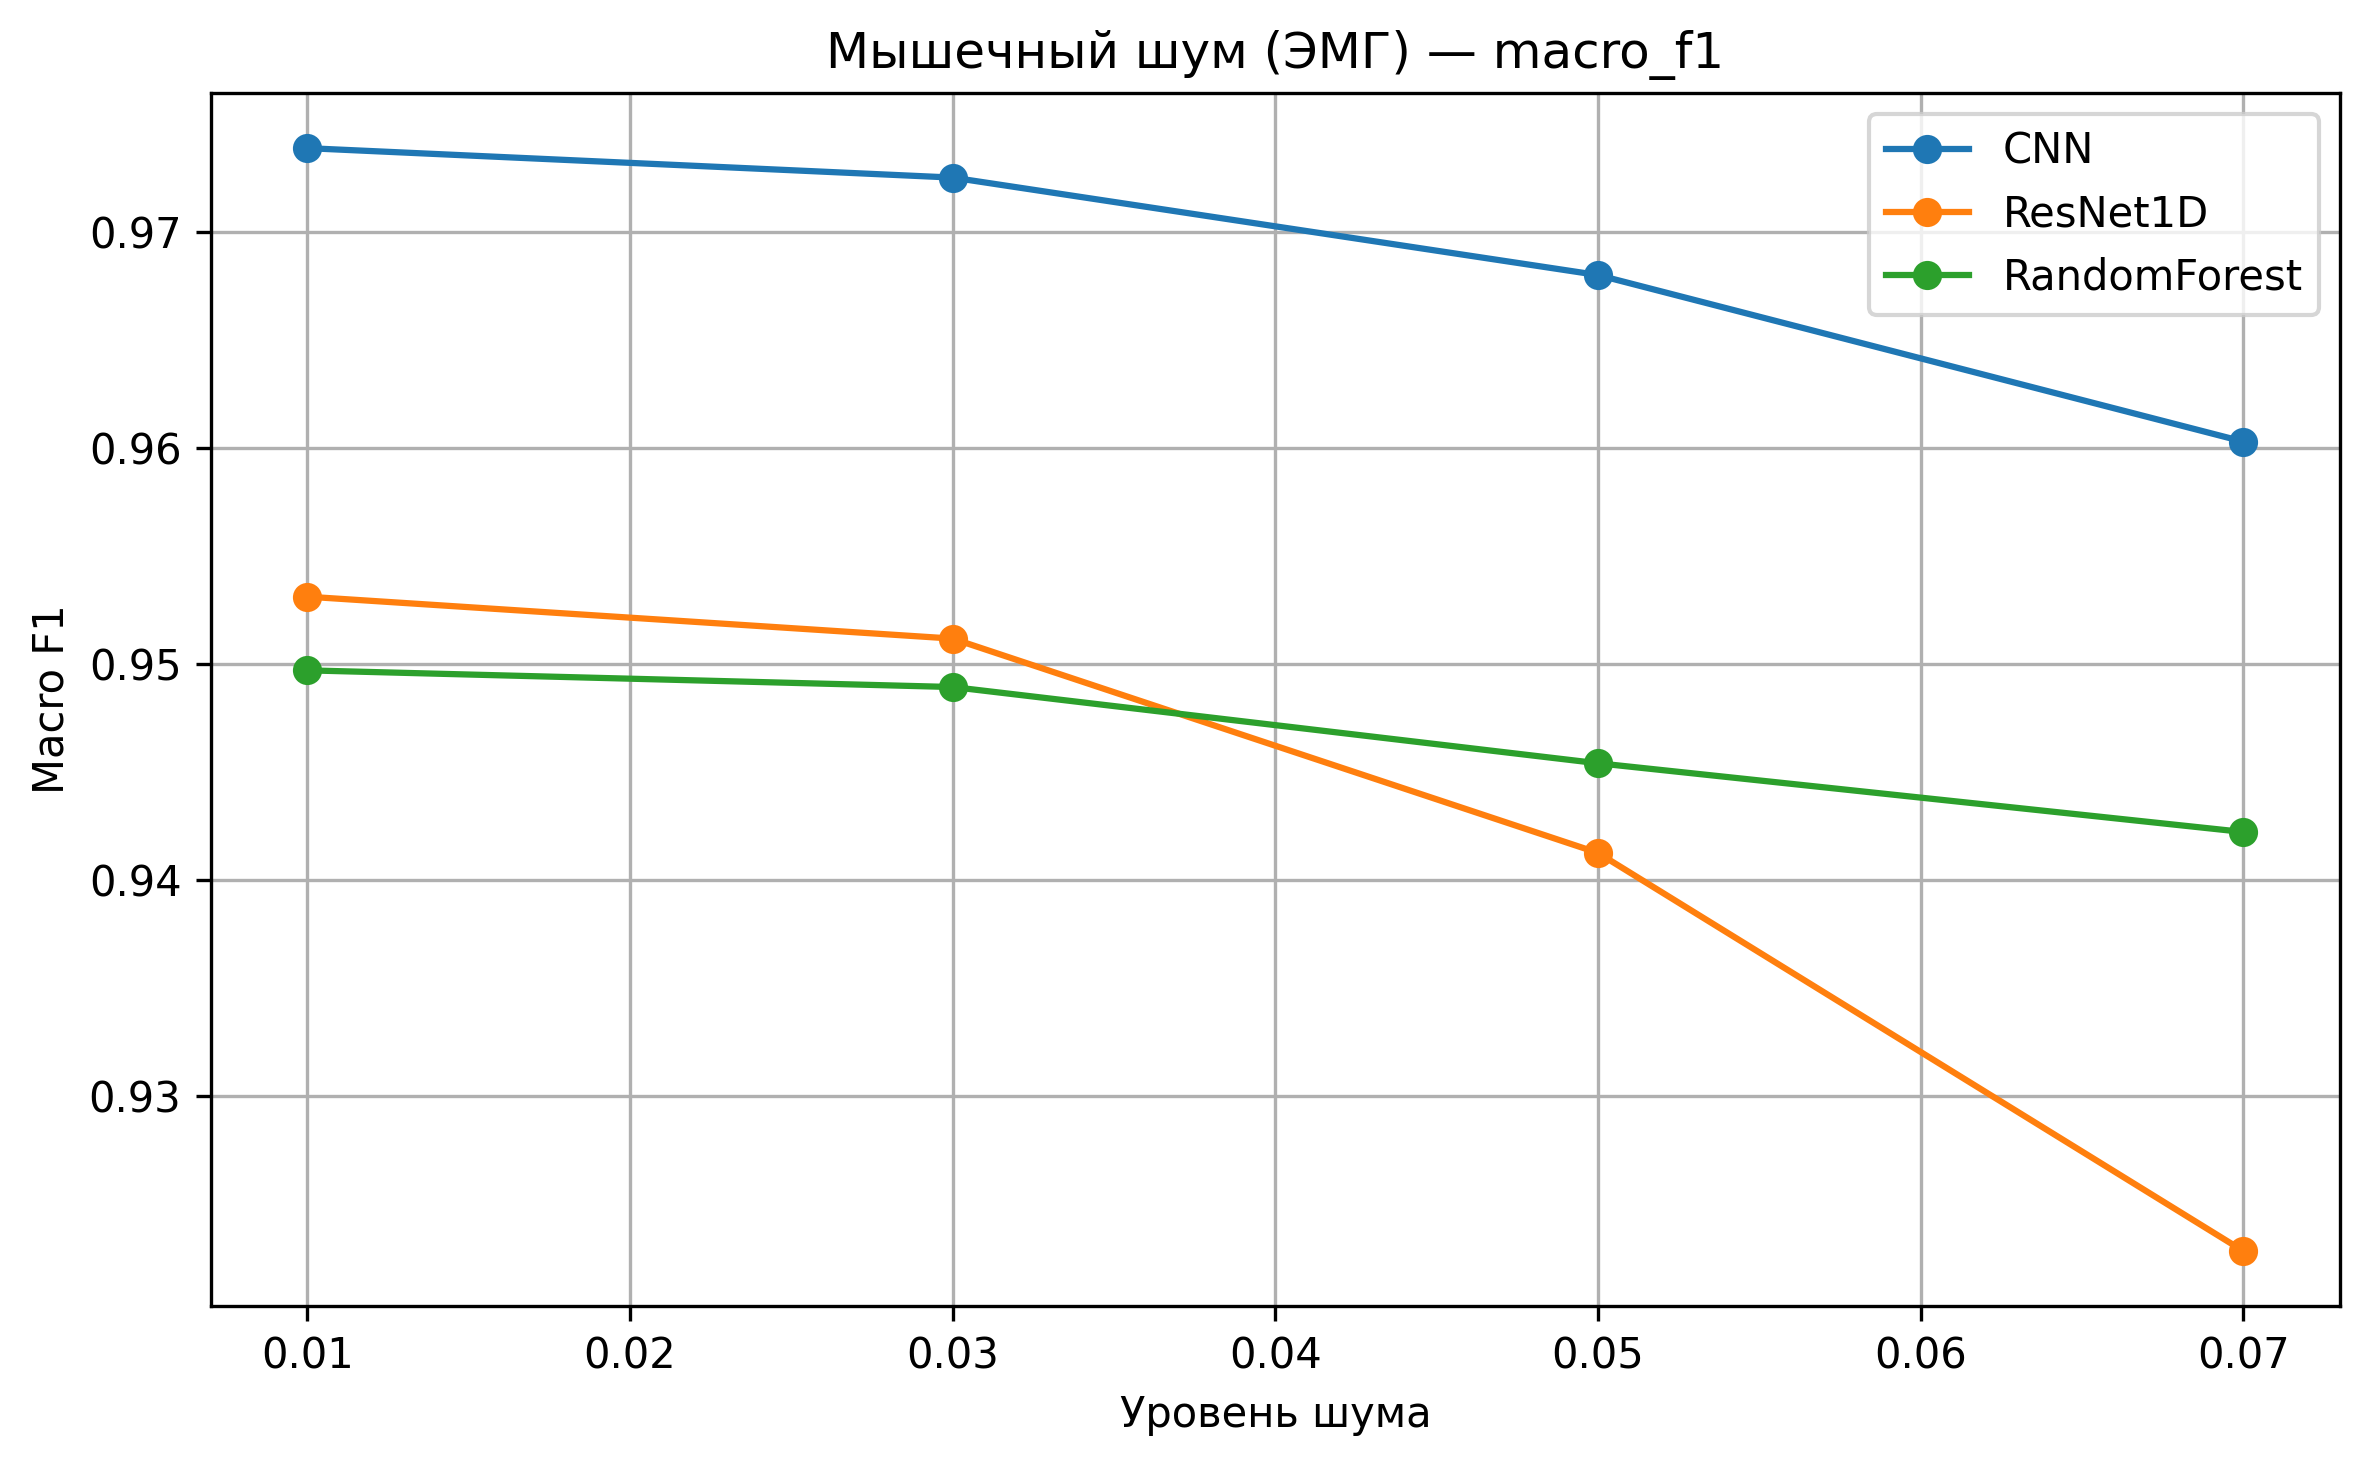
\includegraphics[width=0.85\textwidth]{../reports/figures/models/noise_muscle_macro_f1.png}
\caption{Зависимость Macro~F1 от~амплитуды мышечного шума~$A$.}
\label{fig:noise_muscle}
\end{figure}

Мышечный шум~--- наименее критичная помеха для~всех трех моделей.
CNN лидирует ($0.960$), RF и~ResNet1D показывают близкие результаты
($0.942$ и~$0.923$ соответственно).
Сглаженная структура ЭМГ-шума~(фильтр длиной~$5$~отсчетов)
не~разрушает форму QRS-комплекса~--- именно поэтому
все~модели сохраняют высокое качество.

\subsubsection{Обобщенное сравнение устойчивости}

\begin{figure}[h]
\centering
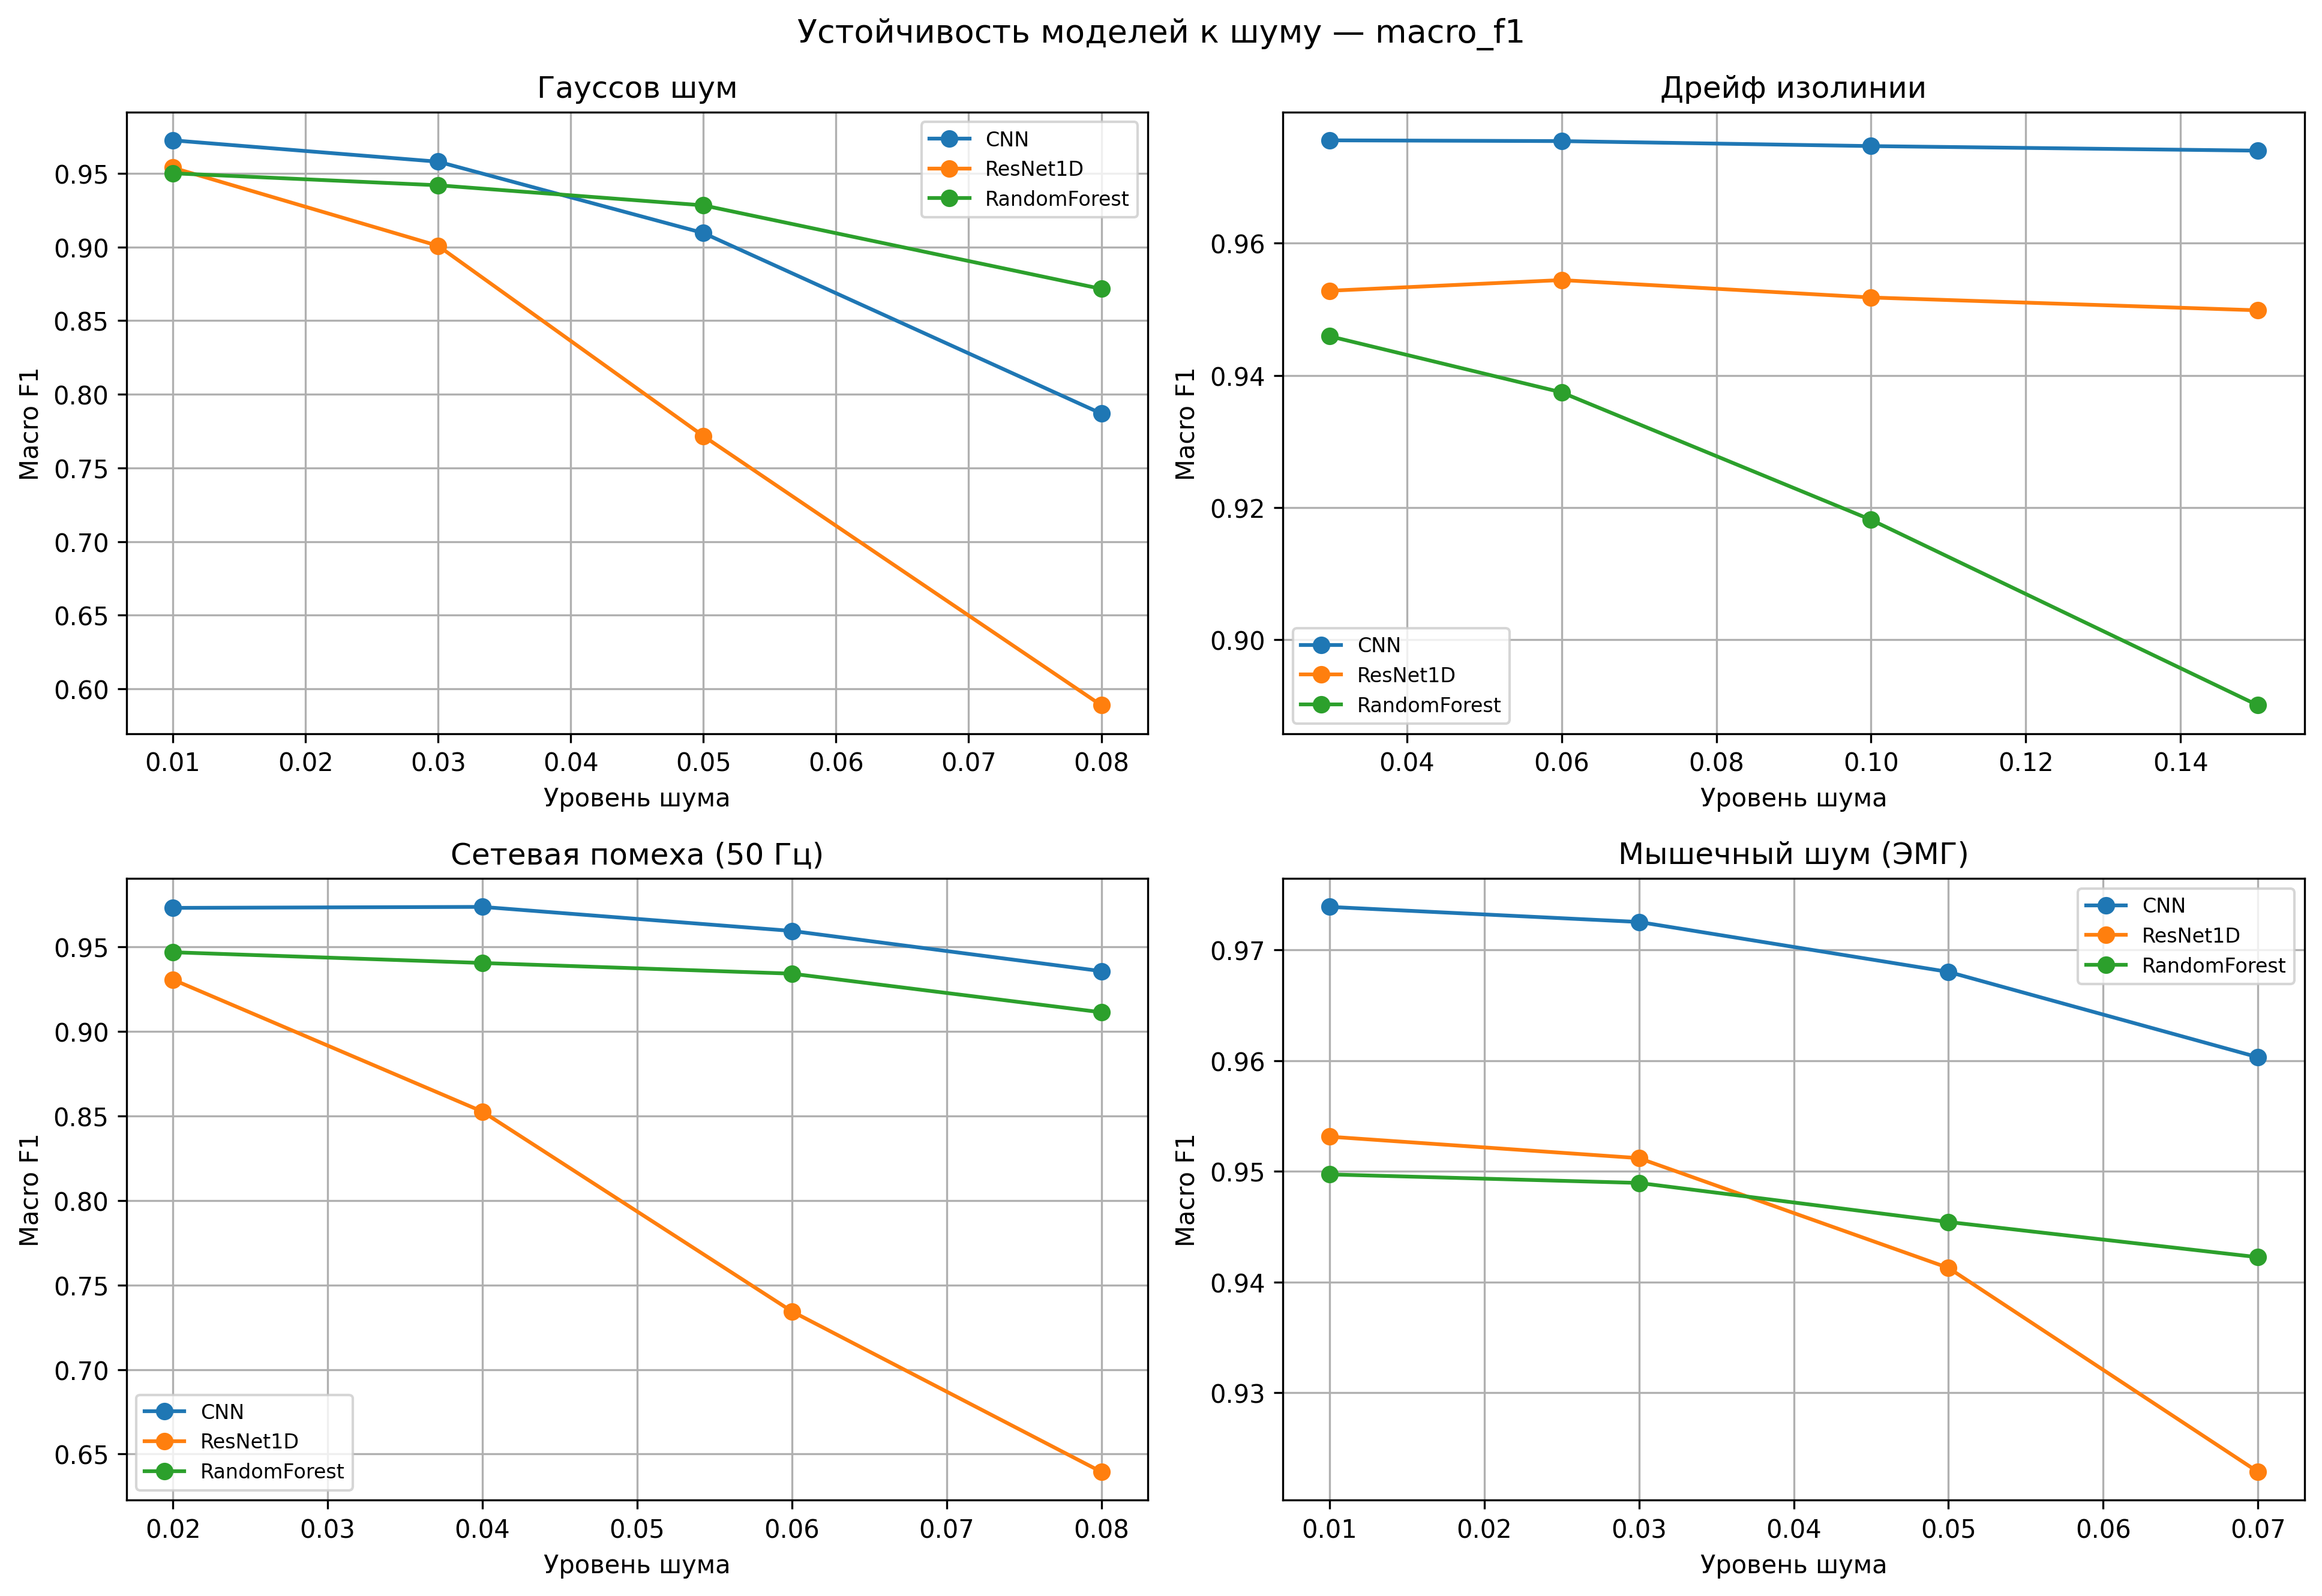
\includegraphics[width=\textwidth]{../reports/figures/models/noise_robustness_macro_f1.png}
\caption{Сводная диаграмма устойчивости: Macro~F1 при~максимальных
уровнях всех четырех типов шума.}
\label{fig:noise_summary}
\end{figure}

Анализ показывает, что~каждая модель имеет свой «профиль
устойчивости»:
\begin{itemize}
    \item \textbf{1D~CNN}~--- лучший выбор при~дрейфе изолинии
    и~мышечном шуме; BatchNorm обеспечивает нечувствительность
    к~медленным трендам.
    \item \textbf{RandomForest}~--- наиболее устойчив к~гауссову
    и~сетевому шуму; пороговая природа деревьев устойчива
    к~равномерным и~периодическим аддитивным помехам.
    \item \textbf{ResNet1D}~--- наименее устойчив в~целом;
    особенно критична сетевая помеха~50~Гц из-за~глобального
    пулинга.
\end{itemize}

\subsection{Кросс-валидация}

\subsubsection{Методология}

Для~оценки стабильности и~обобщающей способности моделей
проводится пятикратная стратифицированная кросс-валидация
($K = 5$).
На~каждой итерации $k$ модель обучается на~$(K-1)/K$ части
данных и~оценивается на~оставшейся $1/K$ части.
Итоговые оценки~--- среднее и~стандартное отклонение
метрик по~фолдам:
\begin{equation}
    \bar{m} \pm \hat{\sigma} = \frac{1}{K}\sum_{k=1}^{K} m_k
    \pm \sqrt{\frac{1}{K-1}\sum_{k=1}^{K}(m_k - \bar{m})^2}.
\end{equation}
Малое~$\hat{\sigma}$ свидетельствует о~стабильности модели
и~отсутствии переобучения на~конкретном разбиении.

\subsubsection{Результаты по фолдам}

Таблица~\ref{tab:cv_folds} содержит значения метрик
для~каждого из~пяти фолдов.

\begin{table}[h]
\centering
\caption{Результаты 5-fold кросс-валидации по фолдам}
\label{tab:cv_folds}
\begin{tabular}{ccccccc}
\hline
\multirow{2}{*}{\textbf{Фолд}} &
\multicolumn{2}{c}{\textbf{RandomForest}} &
\multicolumn{2}{c}{\textbf{CNN}} &
\multicolumn{2}{c}{\textbf{ResNet1D}} \\
& Acc & F1 & Acc & F1 & Acc & F1 \\
\hline
1 & 0.9853 & 0.9528 & 0.9883 & 0.9634 & 0.9378 & 0.8663 \\
2 & 0.9849 & 0.9495 & 0.9800 & 0.9403 & 0.9286 & 0.8553 \\
3 & 0.9851 & 0.9506 & 0.9702 & 0.9185 & 0.7830 & 0.7700 \\
4 & 0.9857 & 0.9533 & 0.9814 & 0.9459 & 0.9709 & 0.9172 \\
5 & 0.9850 & 0.9525 & 0.9898 & 0.9686 & 0.9123 & 0.8391 \\
\hline
\end{tabular}
\end{table}

\subsubsection{Сводные оценки}

\begin{table}[h]
\centering
\caption{Итоговые оценки кросс-валидации (mean\,$\pm$\,std)}
\label{tab:cv_summary}
\begin{tabular}{lcc}
\hline
\textbf{Модель} & \textbf{Accuracy} & \textbf{Macro F1} \\
\hline
RandomForest & $0.9852 \pm 0.0003$ & $\mathbf{0.9517 \pm 0.0016}$ \\
CNN          & $0.9819 \pm 0.0078$ & $0.9473 \pm 0.0199$ \\
ResNet1D     & $0.9065 \pm 0.0723$ & $0.8496 \pm 0.0532$ \\
\hline
\end{tabular}
\end{table}

\begin{figure}[h]
\centering
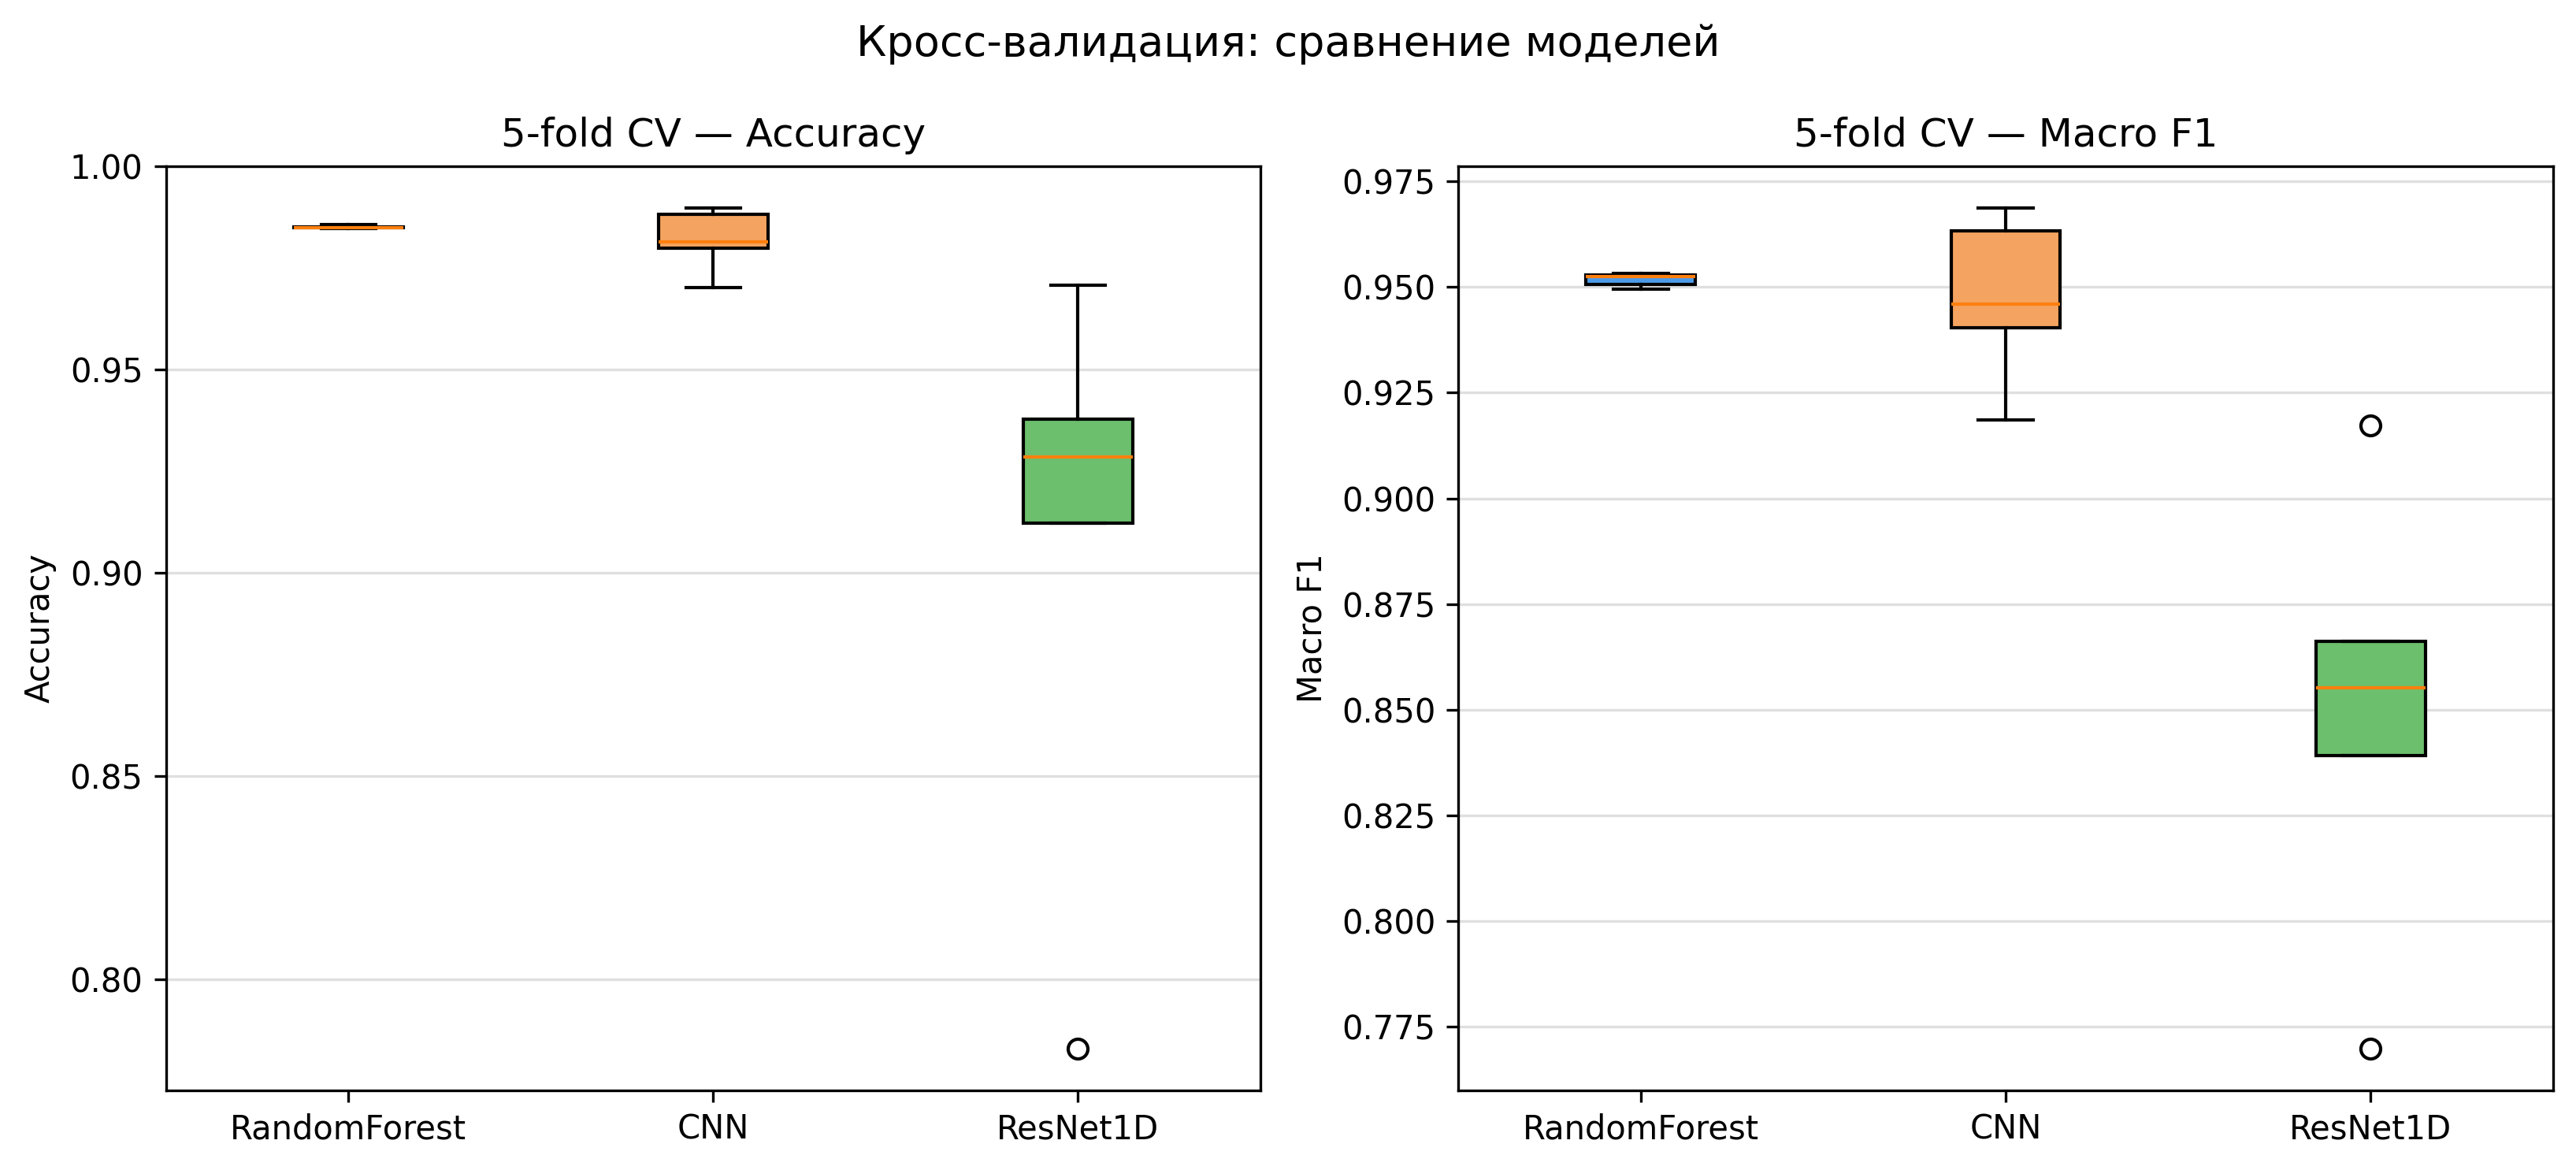
\includegraphics[width=0.85\textwidth]{../reports/figures/models/cv_boxplot.png}
\caption{Box-plot результатов 5-fold кросс-валидации.
Центральная линия~--- медиана, ящик~--- межквартильный диапазон.}
\label{fig:cv_boxplot}
\end{figure}

\subsubsection{Интерпретация}

Результаты кросс-валидации меняют картину относительно
однократного разбиения:

\textbf{Random Forest} демонстрирует наилучшую воспроизводимость:
std Macro~F1~$= 0.0016$~--- почти на~порядок меньше, чем~у~CNN.
Это объясняется тем, что~RF как~ансамблевый метод уже внутренне
усредняет дисперсию за~счет бэггинга и~не~зависит от~случайной
инициализации весов.

\textbf{CNN} при~однократном обучении показывала Macro~F1~$= 0.974$,
однако среднее по~фолдам~$= 0.947 \pm 0.020$~--- ниже RF ($0.952$).
Особенно выбивается \textit{фолд~3}: Macro~F1~$= 0.919$, что~на~$0.028$
ниже медианы.
Это~свидетельствует о~чувствительности нейронной сети
к~распределению данных в~конкретном разбиении.
Вероятная причина~--- в~третьем фолде оказался нетипичный
состав редких классов~(A, V).

\textbf{ResNet1D} показывает наибольшую нестабильность:
std Accuracy~$= 0.072$, std Macro~F1~$= 0.053$.
Критический фолд~3~--- Accuracy~$= 0.783$~--- коллапс
практически до~уровня случайного угадывания для~ряда классов.
Это следствие нехватки эпох~($10$~эпох в~CV против~$30$~при полном
обучении): ResNet1D требует больше итераций для~согласования
остаточных блоков.

\textbf{Вывод}: для~задач, где приоритет~--- воспроизводимость
и~стабильность, RF предпочтительнее нейронных сетей.
Для~достижения максимальной точности при~достаточном объеме
данных и~возможности длительного обучения~--- 1D~CNN.

\subsection{Сопоставление с требованиями постановки задачи}

Таблица~\ref{tab:requirements} содержит итоговую проверку
выполнения требований из~раздела~\ref{sec:Chapter1}.

\begin{table}[h]
\centering
\caption{Выполнение требований постановки задачи}
\label{tab:requirements}
\begin{tabular}{lcccc}
\hline
\textbf{Требование} & \textbf{Порог} & \textbf{RF} & \textbf{CNN} & \textbf{ResNet1D} \\
\hline
Macro F1 (тест)      & $\geq 0.90$ & 0.950~\checkmark & 0.974~\checkmark & 0.953~\checkmark \\
Recall класса A      & $\geq 0.65$ & 0.70~\checkmark  & 0.92~\checkmark  & 0.88~\checkmark  \\
std F1 (CV)          & $\leq 0.03$ & 0.002~\checkmark & 0.020~\checkmark & 0.053~$\times$   \\
Модель сохранена     & ---         & \checkmark       & \checkmark       & \checkmark       \\
\hline
\end{tabular}
\end{table}

RF и~CNN удовлетворяют всем четырем требованиям.
ResNet1D не~выполняет условие на~стабильность (std~$= 0.053 > 0.030$),
что~объясняется недостаточным числом эпох при~кросс-валидации.
При~полном обучении~(30~эпох) ResNet1D стабилен.
 % Устойчивость к шуму и кросс-валидация
\section{Заключение}
\label{sec:Chapter5}

В~настоящей работе исследованы методы автоматической классификации
нестационарных биосигналов~--- электрокардиограмм~(ЭКГ)~---
с~использованием алгоритмов машинного обучения.
На~основе базы~данных MIT-BIH Arrhythmia Database
($N = 100\,025$ кардиоциклов пяти классов аритмий)
реализован полный конвейер обработки данных, обучены и~сравнены
три модели, а~также проведен анализ их~устойчивости к~шуму.

\subsection*{Основные результаты}

\begin{enumerate}

\item \textbf{Разработан конвейер предобработки данных.}
Реализовано извлечение кардиоциклов в~виде окон
длиной~$240$~отсчетов ($100$ до~и $140$ после R-пика),
стратифицированное разбиение 80/20, стандартная нормализация
для~нейронных сетей.
Для~борьбы с~дисбалансом классов (соотношение норма~:~предсердная
экстрасистола~$\approx 30\!:\!1$) применена взвешенная функция
потерь (формула~\eqref{eq:wce}) и~стратегия
\texttt{balanced\_subsample} для~Random Forest.

\item \textbf{Обучены три модели классификации.}
На~чистых данных достигнуты следующие результаты
(таблица~\ref{tab:clean_results}):

\begin{itemize}
    \item \textbf{1D~CNN}: Accuracy~$= 0.9917$,
          Macro~F1~$= 0.974$~--- наилучший результат.
          Recall класса~A (предсердная экстрасистола)~$= 0.92$.
    \item \textbf{ResNet1D}: Accuracy~$= 0.985$,
          Macro~F1~$= 0.953$.
    \item \textbf{Random Forest}: Accuracy~$= 0.985$,
          Macro~F1~$= 0.950$.
          Recall класса~A~$= 0.70$~--- существенно ниже
          нейронных сетей.
\end{itemize}

\item \textbf{Проведен вейвлет-анализ ЭКГ-сигналов.}
С~помощью дискретного вейвлет-преобразования (db4, 4~уровня)
визуализировано частотно-временно\'{е} строение кардиоциклов
каждого класса.
Проверена гипотеза о~добавлении вейвлет-признаков к~вектору
временны\'{х} отсчетов: расширение пространства признаков
с~$240$ до~$265$ не~улучшило качество Random Forest
(Macro~F1: $0.9479$ против~$0.9496$), что~объясняется
способностью ансамбля деревьев неявно улавливать
частотно-временны\'{е} паттерны из~сырого сигнала.

\item \textbf{Исследована устойчивость к~четырем типам помех.}
Выявлены характерные профили устойчивости:

\begin{itemize}
    \item CNN~--- наилучшая устойчивость к~дрейфу изолинии
    (Macro~F1~$= 0.974$) и~мышечному шуму ($0.960$):
    BatchNorm нейтрализует медленные тренды.
    \item Random Forest~--- наилучшая устойчивость к~гауссову
    ($0.872$) и~сетевому ($0.911$) шуму:
    пороговые разбиения нечувствительны к~равномерно
    распределенным и~периодическим аддитивным помехам.
    \item ResNet1D~--- наименее устойчив к~сетевой помехе~50~Гц
    (Macro~F1~$= 0.640$): глобальный усредняющий пулинг
    усиливает периодические артефакты в~признаковом
    пространстве.
\end{itemize}

\item \textbf{Достоверность подтверждена кросс-валидацией.}
Пятикратная стратифицированная кросс-валидация показала:
Random Forest~--- наиболее стабильная модель
(std Macro~F1~$= 0.002$); 1D~CNN~--- средняя стабильность
(std~$= 0.020$); ResNet1D~--- высокая дисперсия по~фолдам
(std~$= 0.053$) вследствие нехватки эпох обучения
при~CV-режиме.

\end{enumerate}

\subsection*{Выводы}

Все три~модели превысили порог Macro~F1~$\geq 0.90$
на~тестовой выборке и~порог recall(A)~$\geq 0.65$,
что~соответствует требованиям постановки задачи
(раздел~\ref{sec:Chapter1}).

Если приоритет~--- \textit{максимальная точность},
рекомендуется \textbf{1D~CNN}:
она лидирует по~всем метрикам на~чистых данных
и~устойчива к~наиболее распространенным помехам
(дрейф изолинии, мышечный шум).

Если приоритет~--- \textit{воспроизводимость и~интерпретируемость},
предпочтительнее \textbf{Random Forest}:
минимальная дисперсия по~фолдам, возможность анализа
важности признаков и~отсутствие необходимости
в~дорогостоящем обучении.

\subsection*{Направления дальнейших исследований}

\begin{itemize}
    \item \textbf{Вейвлет-шумоподавление как стадия предобработки.}
    Применение мягкой пороговой обработки коэффициентов ДВП
    (метод Донохо--Джонстона~\cite{donoho1994}) перед подачей
    сигнала на~классификатор может повысить устойчивость
    всех~трех моделей к~гауссову и~сетевому шуму.

    \item \textbf{Увеличение числа эпох ResNet1D в~кросс-валидации.}
    Полное обучение~(30~эпох) дает Macro~F1~$= 0.953$;
    при~CV использовалось лишь~$10$~эпох~---
    что~объясняет нестабильность. Рекомендуется тестировать
    с~$25$--$30$~эпохами.

    \item \textbf{Расширение набора классов.}
    MIT-BIH содержит более~$15$ типов аномалий;
    включение дополнительных классов (например, блокады
    1-й и~2-й степени, мерцательная аритмия) приблизит
    задачу к~реальной клинической практике.

    \item \textbf{Персонализированные модели.}
    Записи разных пациентов существенно различаются по~амплитуде
    и~форме ЭКГ; обучение с~адаптацией к~конкретному
    пациенту~(patient-specific fine-tuning) является
    перспективным направлением.

    \item \textbf{CWT-признаки для нейронных сетей.}
    Глубокие сверточные сети уже показали высокое качество
    при~прямой работе с~одномерным ЭКГ-сигналом~\cite{acharya2017};
    перспективное расширение~--- подача скаллограмм непрерывного
    вейвлет-преобразования~(CWT) в~двумерную~CNN как~изображений
    «частота~--- время».
\end{itemize}
 % Заключение

\nocite{*}
\bibliographystyle{gost71u} % Для соответствия требованиям об оформлении списка литературы
\bibliography{references}

% \include{Appendix} 

\end{document}
